% Этот шаблон документа разработан в 2014 году
% Данилом Фёдоровых (danil@fedorovykh.ru) 
% для использования в курсе 
% <<Документы и презентации в \LaTeX>>, записанном НИУ ВШЭ
% для Coursera.org: http://coursera.org/course/latex .
% Исходная версия шаблона --- 
% https://www.writelatex.com/coursera/latex/5.3

\documentclass[a4paper,12pt]{article}

%%% Поля и разметка страницы %%%
\usepackage{lscape} % Для включения альбомных страниц
\usepackage{geometry} % Для последующего задания полей
\usepackage{float}

%%% Кодировки и шрифты %%%
\usepackage{cmap} % Улучшенный поиск русских слов в полученном pdf-файле
\usepackage[T2A]{fontenc} % Поддержка русских букв
\usepackage[utf8]{inputenc} % Кодировка utf8
\usepackage[english, russian]{babel} % Языки: русский, английский
%\usepackage{pscyr} % Нормальные шрифты

\usepackage{extsizes} % Возможность сделать 14-й шрифт
\usepackage{anyfontsize}

%%% Математические пакеты %%%
\usepackage{amsthm,amsfonts,amsmath,amssymb,amscd} % Математические дополнения от AMS
\usepackage{icomma} % "Умная" запятая: $0,2$ --- число, $0, 2$ --- перечисление

%%% Оформление абзацев %%%
\usepackage{indentfirst} % Красная строка

%%% Цвета %%%
\usepackage[usenames]{color}
\usepackage{color}
\usepackage{colortbl}

%%% Таблицы %%%
\usepackage{longtable} % Длинные таблицы
\usepackage{multirow,makecell,array} % Улучшенное форматирование таблиц

%%% Общее форматирование
%\usepackage[singlelinecheck=off,center]{caption} % Многострочные подписи
\usepackage{caption2}%форматирование подписей к плавающим объектам
\renewcommand{\captionlabeldelim}{.}% после названия объекта ставим точку.
\usepackage{soul} % Поддержка переносоустойчивых подчёркиваний и зачёркиваний

%%% Библиография %%%
%\usepackage{cite}

%%% Гиперссылки %%%
%\usepackage[plainpages=false,pdfpagelabels=false]{hyperref}
\usepackage[linktocpage=true,plainpages=false,pdfpagelabels=false]{hyperref}

%%% Изображения %%%
\usepackage{graphicx} % Подключаем пакет работы с графикой

%%% Опционально %%%
% следующий пакет может быть полезен, если надо ужать текст, чтобы сам текст не править, но чтобы места он занимал поменьше
%\usepackage{savetrees}        

% этот пакет может быть полезен для печати текста брошюрой, сама с ним не разбиралась
%\usepackage[print]{booklet}

\newcommand{\R}{R} %Rlogo

\usepackage{wasysym}

%%%%%%%%%%%%%%%%%%%%%%%%%%%%%%%%%%%%%%%%%%%%%

%%% Макет страницы %%%


%\geometry{top=1.5cm,bottom=1.5cm,left=1.5cm,right=1cm}
\geometry{top=1.5cm,bottom=1.5cm,left=2cm,right=1.5cm}
%\oddsidemargin=-13pt
%\topmargin=-66pt
%\headheight=12pt
%\headsep=38pt
%\textheight=732pt
%\textwidth=484pt
%\marginparsep=14pt
%\marginparwidth=43pt
%\footskip=14pt
%\marginparpush=7pt
%\hoffset=0pt
%\voffset=0pt
%\paperwidth=597pt
%\paperheight=845pt
\parindent=1cm %размер табуляции (для красной строки) в начале каждого абзаца
\renewcommand{\baselinestretch}{1.25}
%\newfloat{scheme}{tb}{sch}

%%% Общая информация %%%
\author{Назарова С.А.} % Фамилия И.О. автора

%%% Кодировки и шрифты %%%
%\renewcommand{\rmdefault}{ftm} % Включаем Times New Roman

%%% Выравнивание и переносы %%%
\sloppy
\clubpenalty=10000
\widowpenalty=10000

%%% Библиография %%%
%\makeatletter
%\bibliographystyle{utf8gost705u} % Оформляем библиографию в соответствии с ГОСТ 7.0.5
%\renewcommand{\@biblabel}[1]{#1.} % Заменяем библиографию с квадратных скобок на точку:
%\makeatother

%%% Изображения %%%
\graphicspath{{images/}} % Пути к изображениям

%%% Цвета гиперссылок %%%
\definecolor{linkcolor}{rgb}{0,0,0}
\definecolor{citecolor}{rgb}{0,0,0}
\definecolor{urlcolor}{rgb}{0,0,0}
\hypersetup{
    colorlinks, linkcolor={linkcolor},
    citecolor={citecolor}, urlcolor={urlcolor}
}


%это движок biber
%\usepackage[backend=biber,bibencoding=utf8,sorting=nyt,maxcitenames=2,style=authoryear]{biblatex}

%biblatex-gost
\usepackage[backend=biber, style=gost-authoryear, language=auto, babel=other, bibencoding=utf8, bibdoi=false, biburl=false, movenames=false]{biblatex}

\addbibresource{sophia_base.bib}

%\includeonly{chapters/ch2,chapters/ch3}

\begin{document} % конец преамбулы, начало документа

%%титульный лист
\thispagestyle{empty}

\begin{center}
САНКТ-ПЕТЕРБУРГСКИЙ ГОСУДАРСТВЕННЫЙ УНИВЕРСИТЕТ\par
%БИОЛОГИЧЕСКИЙ ФАКУЛЬТЕТ\par
%КАФЕДРА ИХТИОЛОГИИ И ГИДРОБИОЛОГИИ\par  
\par
\end{center}

\vspace{20mm}
\begin{flushright}
На правах рукописи

%{\sl УДК xxx.xxx}
\end{flushright}

\vspace{30mm}
\begin{center}
{\large НАЗАРОВА\\ София Александровна}
\end{center}

\vspace{5mm}
\begin{center}
{\bfseries \large ОРГАНИЗАЦИЯ ПОСЕЛЕНИЙ {\itshape Macoma~balthica}~(Linnaeus,~1758) В ГРАДИЕНТАХ КЛЮЧЕВЫХ ПЕРЕМЕННЫХ СРЕДЫ ОСУШНОЙ ЗОНЫ БЕЛОГО И БАРЕНЦЕВА МОРЕЙ
\par}

\vspace{10mm}
{%\small
Специальность 03.02.10~---

<<Гидробиология>>
}

\vspace{10mm}
Диссертация на соискание учёной степени

кандидата биологических наук
\end{center}

\vspace{20mm}
\begin{flushright}
Научный руководитель:

д.б.н., профессор

Максимович Н.В.

\end{flushright}

\vspace{20mm}
\begin{center}
{Санкт-Петербург  -- 2014}
\end{center}

\newpage


\tableofcontents

%%Введение

%%материал и методика
\chapter{Материал и методика}
	\section{География исследований}
Географическое распространение вида {\it M.~balthica} охватывает бореальную зону Атлантического и Тихого океанов.
В Европейской части ареала {\it M.~balthica} заходит в арктические моря, и встречается в Норвежском, Баренцевом, Белом и Карском морях.
Наиболее северной точкой считается Шпицберген (\cite{Zacepin_Filatova_1968}).
Таким образом, Белое и Баренцево моря являются краевой частью ареала для маком.
		\subsection{Белое море}
В вершине Кандалакшского залива наблюдения проводили на $6$ участках в рамках работы экспедиций Группы исследований прибрежных сообществ Лаборатории экологии морского бентоса (гидробиологии) СПбГДТЮ (рис.~\ref{ris:karta_White}). 
	\begin{figure}[p]
    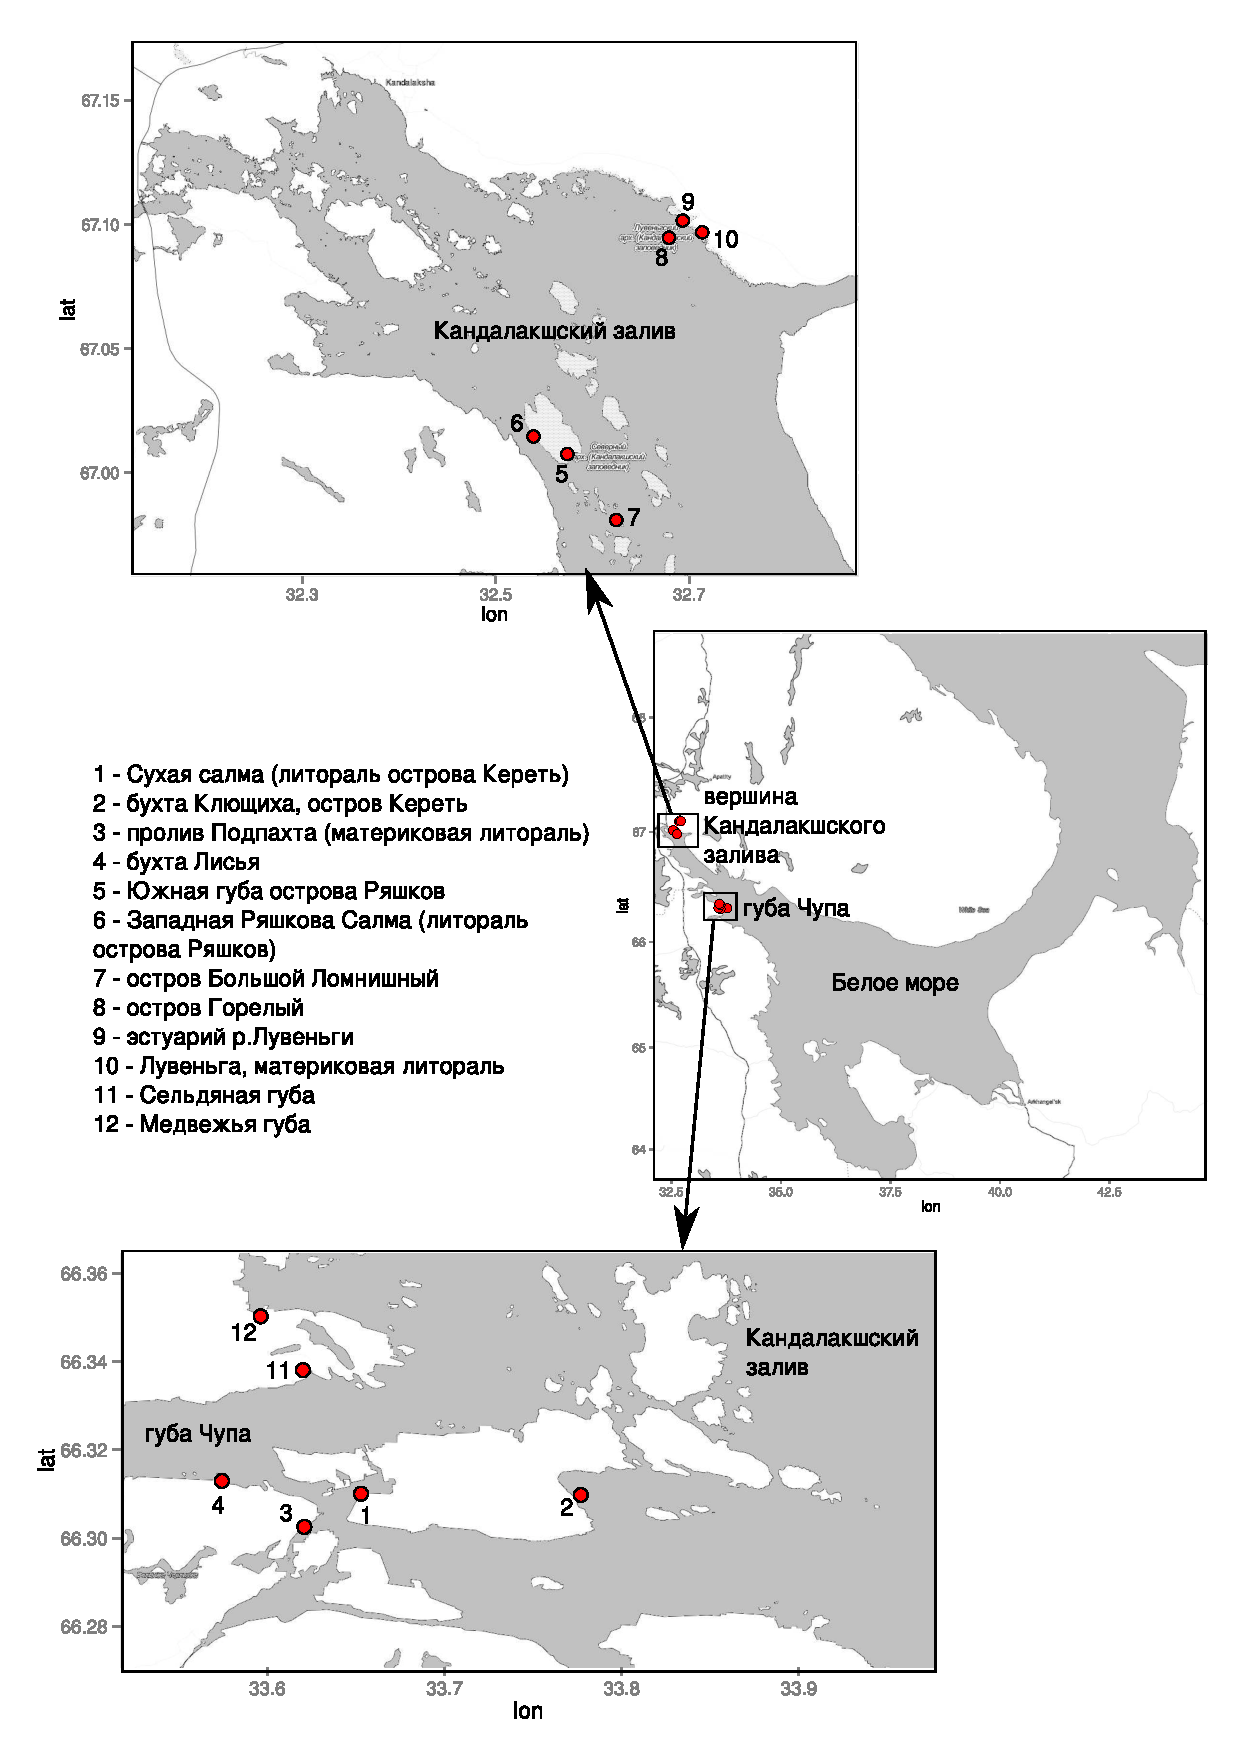
\includegraphics[width=\textwidth]{../maps/White_sea1.pdf}
    \caption{Исследованные участки в Кандалакшском заливе Белого моря}
    \label{ris:karta_White}
	\end{figure}
Три участка расположены в районе Лувеньгских шхер: эстуарий реки Лувеньги, Илистая губа острова Горелого и участок материковой литорали в $800$ метрах западнее поселка Лувеньга (участки 1, 2 и 3).
Один участок был расположен на литорали острова Ряшков в Западной Ряшковой Салме (Северный архипелаг) (участок 4).
В работе использованы данные Д.\:А.~Аристова из Южной губы о.~Ряшков и с о.~Большой Ломнишный (Северный архипелаг) (рис.~\ref{ris:karta_White}, участки 5 и 6). 

В районе губы Чупа исследования проводили на $4$ участках (рис.~\ref{ris:karta_White}) в ходе экспедиций кафедры ихтиологии и гидробиологии СПбГУ. 
Два участка были расположены на литорали острова Кереть~--- в Сухой Салме и бухте Клющиха (участки 7 и 8). 
Один участок был расположен на материковой литорали пролива Подпахта и один --- в бухте Лисьей (участки 9 и 10).

%Также в работе использованы данные ББС <<Картеш>> ЗИН РАН по обилию маком в губах Медвежья и Сельдяная (\cite{Varfolomeeva_Naumov_2013}) (рис.~\ref{ris:karta_White}, участки 11 и 12).

Все карты созданы с использованием данных OpenStreetMap (www.openstreetmap.org).
\afterpage{\clearpage}

		\subsection{Баренцево море}
Материал  в акватории Баренцева моря  был  собран    в ходе   студенческой баренцевоморской экспедиции СПбГУ. 
Всего было исследовано $8$ участков~--- $2$ в Кольском заливе и   $6$  в   прибрежной   зоне  Восточного  Мурмана (рис.~\ref{ris:karta_Barents}).  
	\begin{figure}[p]
    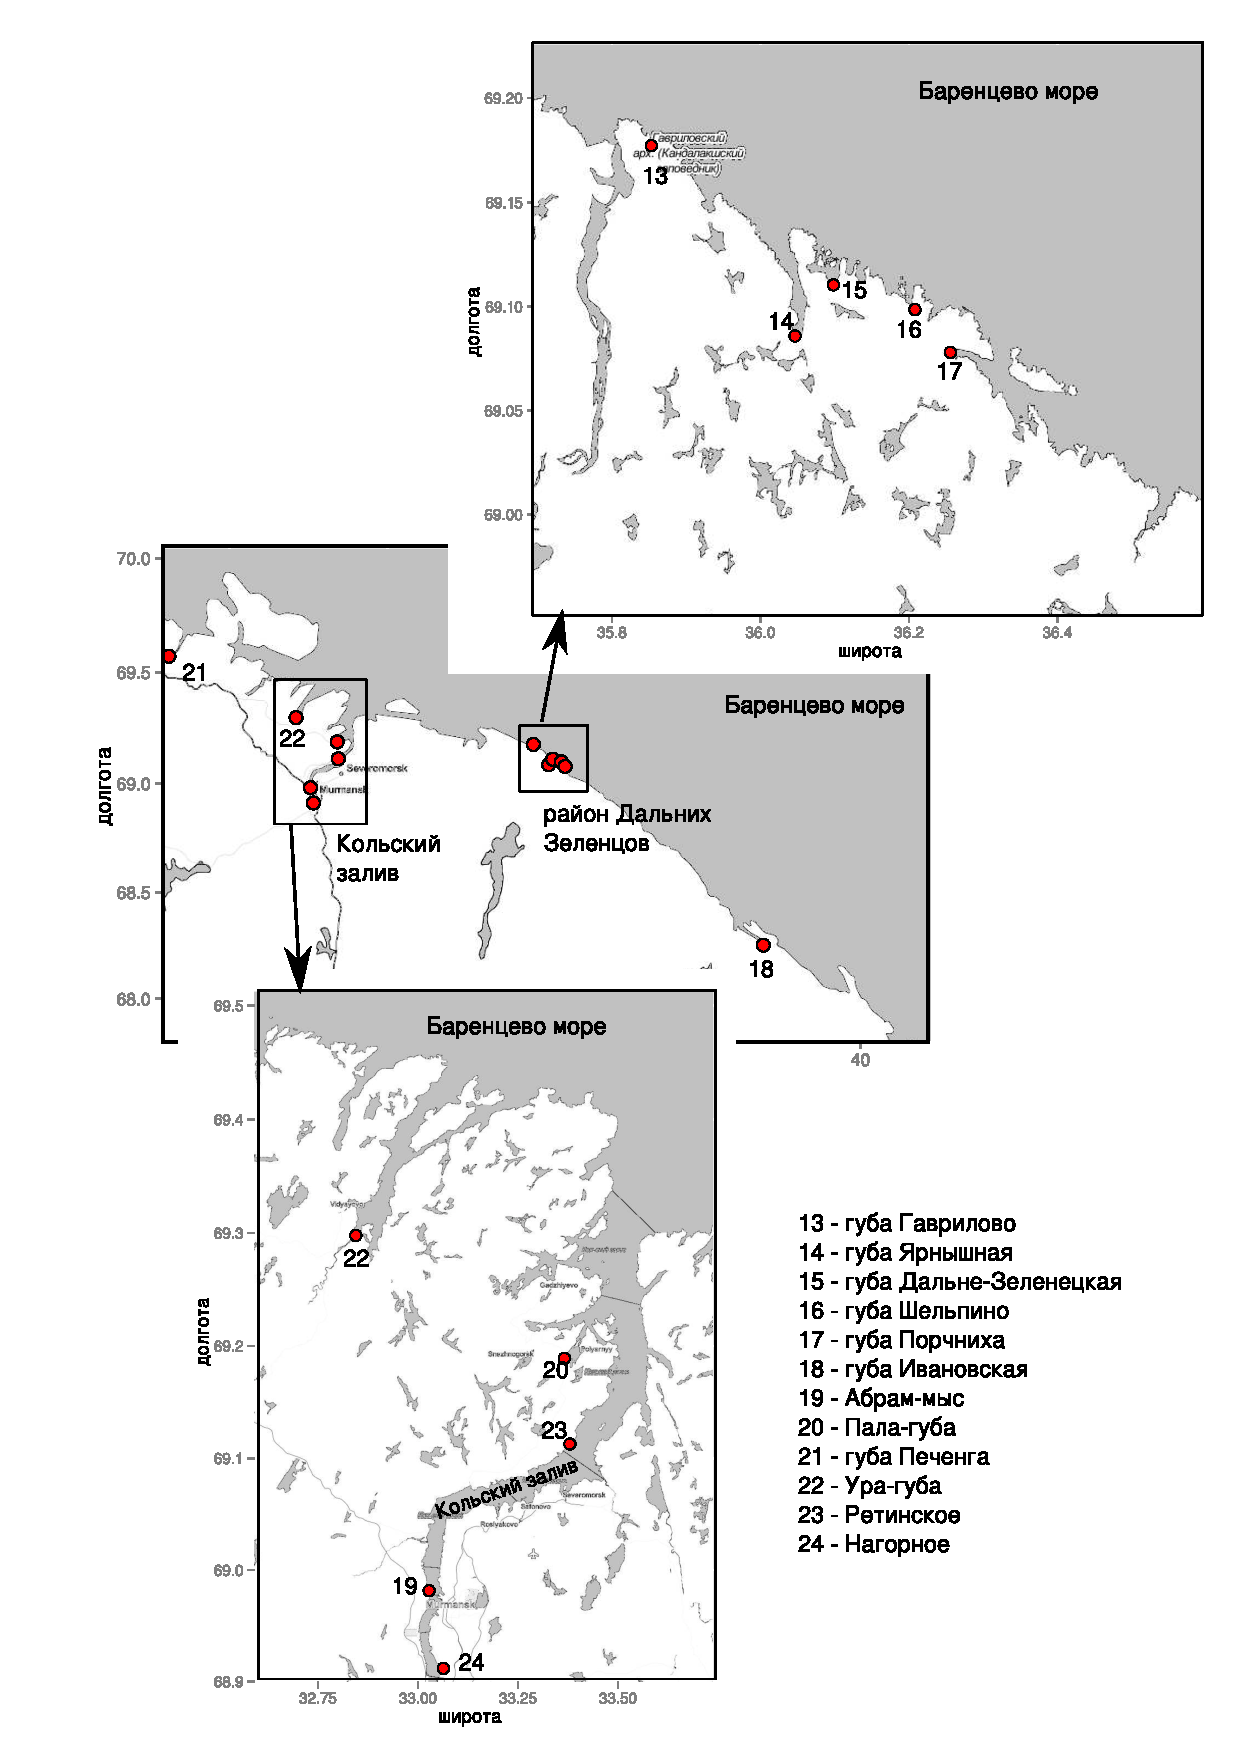
\includegraphics[width=\textwidth]{../maps/Barents_sea1.pdf}
    \caption{Исследованные участки вдоль Мурманского побережья Баренцева моря}
    \label{ris:karta_Barents}
	\end{figure}
На   Восточном   Мурмане исследованные участки литорали  были   расположены   в   губах   Гавриловская (участок 13),  Ярнышная (участок 14), Дальне-Зеленецкая (участок 15), Шельпинская (участок 16), Порчниха (участок 17) и Ивановская (участок 18).
Участки литорали  в   Кольском   заливе   были  расположены на побережье в районе Абрам-мыса (участок 19) и в Палa-губе (участок 20), в районе города Полярный. 


Также в работе использованы данные К.\:В.~Шунькиной и Е.\:А.~Генельт-Яновского по обилию маком в губе Печенга и Ура-губе (Западный Мурман) (рис.~\ref{ris:karta_Barents}, участки 21 и 22), и в районе Северного Нагорного и Ретинского (Кольский залив) (рис.~\ref{ris:karta_Barents}, участки 23 и 24).

\afterpage{\clearpage}

    \section{Характеристика местообитаний}
Для всех участков было составлено физиономическое описание.
На каждом участке измеряли ширину литорали.
По горизонтам описывали визуально тип грунта, наличие валунов, бурых водорослей, взморника \textit{Zostera marina}, зеленых нитчатых водорослей. 
Также описывали поясность сообществ, если она была выражена.
Термогалинные характеристики для отдельных участков не были описаны, и мы использовали литературные данные о среднегодовых параметрах для акваторий, и опубликованные данные о динамике температур в исследованный период (\cite{KGZ_letopis, rp5_Kandalaksha, pinro}.

Показательной комплексной оценкой гидродинамики региона и условий питания детритофагов служат показатели состава грунта. 
Поэтому на ряде исследованных участков были отобраны образцы грунта. 
В Белом море грунт исследовали на обоих участках в губе Чупа и на трех участках в вершине Кандалакшского залива.
В Баренцевом море грунт исследовали на всех участках Восточного Мурмана и двух участках Кольского залива (Абрам-мыс и Пала-губа).

Пробы грунта отбирали на всех исследованных горизонтах каждого участка.
В экспедиции после отбора из грунта выбирали крупных животных (червей, раков, моллюсков, приапулид), образцы высушивали и упаковывали для отправки в город. 
В городе образцы досушивали в термостате при температуре $105^o$C до момента, когда масса образца переставала изменяться. 
Из каждого образца брали по три навески грунта для определения содержания органических веществ. 
Навески помещали в муфельную печь с температурой $450^o$C на $8$ часов. 
После сжигания навески повторно взвешивали, и по разнице масс определяли массовую долю органических веществ в грунте. 
По трем навескам рассчитывали среднюю массовую долю для каждого образца.

Оставшийся грунт использовали для определения гранулометрического состава. 
При описании гранулометрического состава грунта использовали классификацию И.\,Л.~Безрукова и А.\,Н.,~Лисицина для морских водоемов (таблица~\ref{tab:lisicyn_granulometriya}, \cite{Bezrukov_Lisicyn_1960}).
\begin{table}[p]
    \centering
    \caption{Классификация фракций грунта по размеру частиц (\cite{Bezrukov_Lisicyn_1960})}
    \label{tab:lisicyn_granulometriya}
\begin{tabular}{|l|l|}
    \hline
    Размер фракции,~мм & Название фракции         \\ \hline
     $> 10$    & Крупный и средний гравий  \\
    $10-5$               & Мелкий гравий         \\
    $5-3$                & Очень мелкий гравий   \\
    $3-1$                & Очень крупный песок   \\
    $1-0,5$              & Крупный песок         \\
    $0,5-0,25$           & Средний песок         \\
    $0,25-0,1$           & Мелкий песок          \\
    $< 0,1$           & алевриты       \\\hline
\end{tabular}
\end{table}
Для этого грунт взвешивали, после чего просеивали в сухом состоянии через колонку сит (диаметр ячеи: $10 - 5 - 3 - 1 - 0,5 - 0,25$~мм). 
Частицы размером менее $0,25$~мм просеивали через сито с диаметром ячеи $0,1$~мм с использованием струи воды, после чего оставшиеся на сите --- высушивали при температуре $105^o$C. 
Каждую фракцию частиц взвешивали, и определяли их массовую долю. 
Анализ частиц размером менее $0,1$~мм (алевритов)не проводили. 

\afterpage{\clearpage}

    \section{Описание сообществ, включающих {\it Macoma balthica}}
На 6 мониторинговых участках в Кандалакшском заливе Белого моря проводили качественное описание фауны в пределах обследованных горизонтов литорали.
Таким образом, всего составлено $12$~описаний.
На каждом участке в акватории Баренцева моря исследовали все  горизонты литорали, представленные мягкими грунтами.  
Таким образом, всего было составлено $16$ описаний.

Как основное орудие сбора использовали литоральную рамку площадью $1/30$~м$^2$, из которой изымали грунт на глубину $5$~см. 
В случае, когда приходилось отбирать пробы из-под воды, использовали зубчатый водолазный дночерпатель площадью захвата $1/20$~м$^2$.
Отобранные пробы промывали на сите с диаметром ячеи $1$~мм. 

После промывки из   проб   выбирали   всех   особей  {\it M.~balthica}  и   представителей   сопутствующего макрозообентоса    для   определения   состава   сообщества.
Представителей   сопутствующего макрозообентоса  определяли   до   минимально   возможного   таксона. Таксономию и номенклатуру сверяли по Всемирному регистру морских видов (\cite{WoRMS}).

Для сравнения видового состава сообщества использовали коэффициент Жаккара. 
Результаты визуализировали при помощи  кластерного анализа методом ближайшего соседа. 
Достоверность выделенных групп оценивали с помощью анализа сходства профилей (SIMPROF) (\cite{Clarke_et_al_2008}).
Для оценки влияния факторов использовали многомерное шкалирование MDS в сочетании с анализом сходства ANOSIM.
Анализы проводили в программе PaSt (\cite{Hammer_et_al_2001}) и \R{} (\cite{R_2014}).

Кроме того, на литорали губы Дальне-Зеленецкой в $2002 - 2007$ проводили описание структуры сообщества. 
Для этого  в $2002$ году была заложена сеть из 8 станций (\cite{Genelt_Dalnezeleneckaya_2008}).
В пределах каждой станции отбирали 3 пирамиды рамок 1/245 + 1/30~м$^2$. 
Пробы площадью 1/245~м$^2$ промывали на сите с диаметром ячеи $0,5$~мм, внешние пробы площадью 1/30~м$^2$~--- на сите с диаметром ячеи 1~мм.  
Для проб площадью 1/245~м$^2$ проводили полную количественную разборку с последующей таксономический идентификацией особей и их подсчетом. 
В пробах  площадью 1/30~м$^2$ учитывали крупные виды Polychaeta и всех Bivalvia. 
Также в районе каждой станции отбирали по 3-5 проб площадью 1/10~м$^2$, которые также промывали на сите с диаметром ячеи 1~мм, для учета двустворчатых моллюсков.  У всех двустворчатых моллюсков измеряли длину раковины с точностью 0,1~мм.
Для выделения сообществ использовали анализ сходства профилей (SIMPROF) по матрицам коэффициентов Брея-Кертиса (данные по численности видов) (\cite{Clarke_et_al_2008}). 
Для множественного сравнения средних использовали непараметрический тест Краскела-Уоллиса.
Сравнение современных значений плотности поселений со значениями $1973$ года проводили, оценивая $2,5$ и $97,5$~\% квантили распределений плотности поселений в 2002-2007 годах.


%	\subsection{Изучение микрораспределения {\it Macoma balthica}}

%\textcolor{red}{квадраты на Белом}

%\textcolor{red}{квадраты на Баренцевом}
%При оценке распределения особей в губе Порчниха в 2007 г. было отобрано 32 пробы рамкой 1/30м2, причем пробы брались вплотную друг к другу 4 рядами по 8 шт.

% из Генельт-Кобылков-Назарова, 2007 (что это было??)
%Изучение распределения особей {\it Macoma balthica} было проведено в Баренцевом море по методике, описанной Трашем (\cite{Thrush_et_al_1989}) с изменением масштаба.
%Исследования были проведены в августе $2007$~г. на илисто-песчаной литорали кутовых участков губ Восточного Мурмана --- Ярнышной и Дальне-Зеленецкой, и в октябре $2007$~г. на литорали Пала-губы (Кольский залив). 
%Для Дальне-Зеленецкой губы съемка была повторена в августе $2008$ года на полигоне двойного размера.

%В каждой точке отбиралось по $36$ проб площадью $1/30$~м$^2$, расположенных в пределах участка размером $7,5 \times 12$~м. 
%Координаты каждой пробы были определены в декартовой системе координат в метрах, один из углов участка служил точкой отсчета. 
%В дальнейшем пробы промывали на сите с диаметром ячеи $1$~мм. 
%В лаборатории были выбраны и  подсчитаны все макомы.

%При дальнейшей обработке данных для каждого участках подсчитывали индекс структурности (отношение дисперсии к средней арифметической). 
%Для анализа размеров агрегаций были построены коррелограммы, основанные на коэффициенте пространственной автокорреляции Морана (\cite{ncf}).
%Достоверность коэффициентов определяли пермутационным методом.
%Наличие градиентов проверяли с использованием корреляционного анализа Кендалла между координатами проб и обилием вида в каждой пробе. 
%Все статистические анализы проводили в статистической среде \R{} (\cite{R_2014}) с $95\%$ доверительной вероятностью ($P < 0,05$).
%Для интерпретации результатов корреляционного анализа были использовали пузырьковые диаграммы.

\afterpage{\clearpage}	

	\section{Изучение структуры поселений {\it Macoma balthica}}
Для описания структуры поселений использовали данные всех доступных сборов.

В Белом море всего было обследовано $10$ участков в акватории Кандалакшского залива. 
На шести из них наблюдения проводили на всех горизонтах литорали, представленных мягкими грунтами.
На четырех других были обследованы отдельные горизонты. 

Для Баренцева моря были использованы данные по обилию с $12$ участков. 
На каждом участке в акватории Баренцева моря исследовали все  горизонты литорали, представленные мягкими грунтами.  

Как основное орудие сбора использовали литоральную рамку площадью $1/30$~м$^2$, из которой изымали грунт на глубину $5$~см. 
В случае, когда приходилось отбирать пробы из-под воды, использовали зубчатый водолазный дночерпатель площадью захвата $1/20$~м$^2$.
Отобранные пробы промывали на сите с диаметром ячеи $1$~мм или $0,5$ (на трех мониторинговых участках в районе Лувеньги и в Западной Ряшковой Салме, участки $7, 8 - 10$ на рис.~\ref{ris:karta_White}). 
После промывки из   проб   выбирали   всех   особей  {\it M.~balthica}.
Подробная информация о количестве проб и размере учетных площадок для каждого участка представлены в приложении~\ref{app:NB_table}.

В дальнейшем подсчитывали количество особей в пробах, которое пересчитывали в плотность поселения моллюсков на квадратный метр. 
Для всех средних значений рассчитывали точность учета $d,\% = m/M$, где $m$~--- стандартная ошибка средней, $M$~--- средняя арифметическая.
Биомассу определяли путем взвешивания на весах с точностью 10 мг, либо, для части участков на Белом море, расчетным методом.
Мы использовали формулу зависимости массы макомы от ее длины $W = 0,00016 \times L^{2,96}$, полученную для губы Чупа (\cite{Maximovich_et_al_1993}).


Изучение размерной структуры поселений маком проводили на всех участках.
Для этого у всех моллюсков в пробах под бинокуляром измеряли максимальный линейный размер (длину) с точностью $0,1$~мм.
По полученным данным строили размерно-частотное распределение с шагом $1$~мм.

%Кроме того, на части участков у моллюсков подсчитывали количество меток зимней остановки роста, которое принимали как возраст моллюсков --- число прожитых зим (например, $4+$ это  особи возрастом от $4$ до $5$ лет).   
%Таким   образом   были   получены   оценки возрастной структуры поселений {\it M. balthica}.

Для визуализации данных по обилию использовали графики Тьюки (Tukey boxplots, \cite{Tukey_1977}). 
Сравнение обилия проводили с помощью непараметрического теста Краскела-Уоллиса. 
Для выявления связи величин обилия с гранулометрическим составом грунта использовали непараметрическую корреляцию Спирмена (\cite{Hollander_et_al_2013}).
Классификацию размерных структур проводили с помощью анализа главных компонент (\cite{Mardia_et_al_1979}).
Все анализы проводили в статистической среде \R{} (\cite{R_2014}).

\afterpage{\clearpage}

	\section{Изучение динамики поселений {\it Macoma balthica}}
        \subsection{Белое море}
В Белом море динамику поселений {\it Macoma balthica} исследовали на $6$ участках в районе вершины Кандалакшского залива. 

Сборы проводили с 1992 по 2012 год ежегодно в июле-августе.
Автор принимала участие в полевых сборах с $1999$ по $2007$ год.
Данные за другие годы взяты из архива ГИПС ЛЭМБ.

Структура материала представлена в таблице \ref{tab:material_Kandalaksha}.
\begin{table}[p]
\caption{Структура материала по динамике поселений {\it Macoma balthica} вершины Кандалакшского залива}
\label{tab:material_Kandalaksha}
%\begin{tabular}{|*{5}{p{0.2\textwidth}|}} \hline
    \begin{tabularx}{\textwidth}{|*{5}{X|}} \hline
участок & годы наблюдения & обследованные горизонты литорали & количество проб в однократной съемке & площадь пробоотборника, м$^2$  \\ \hline
о. Горелый Лувеньгских шхер & 1992 -- 2012 & ВГЛ, СГЛ, НГЛ & 1-3 & 1/30, 1/10 \\ \hline
Материковая литораль в районе пос. Лувеньга & 1992-2000, 2002, 2004 & ВГЛ, СГЛ, НГЛ & 12-20 & 1/30 \\ \hline
Эстуарий р. Лувеньги & 1992 -- 2012 & СГЛ & 3 & 1/10 \\ \hline
Литораль Западной Ряшковой Салмы о. Ряшкова & 1994 -- 2012 & СГЛ & 2 & 1/10 \\ \hline
Южная губа о. Ряшкова & 2001 -- 2012 & НГЛ & 9-16 & 1/30 \\ \hline
о. Ломнишный & 2007 -- 2012 & НГЛ & 5-10 & 1/30  \\ \hline
\end{tabularx}
\end{table}

На каждом исследованном участке отбирали $3 - 25$ проб площадью $1/30 - 1/10$~м$^2$, которые затем промывали на сите с диаметром ячеи $0,5 - 1$~мм. 
В пробах учитывали всех особей {\it M.~balthica}, у которых в дальнейшем измеряли максимальный линейный размер (длину) с точностью ~0,1~мм. 

Для определения биомассы моллюсков взвешивали на электронных весах с точностью до $1$~мг. 
Для серий проб, где не проводили взвешивание моллюсков, биомассу определяли расчетным методом с использованием аллометрической зависимости сырой массы маком от длины их раковины (\cite{Maximovich_et_al_1993}). 

В дальнейшем рассчитывали среднюю плотность поселений и строили размерно-частотное распределение особей.
Для построения размерно-частотного распределения шаг размерного класса составлял $1$~мм.

В дальнейшем при анализе мы работали с особями с длиной раковины более $1,0$~мм по двум причинам. 
Во-первых, для того чтобы сделать сравнимыми результаты с разных участков, где пробы промывались на ситах с разным диаметром ячеи. 
Во-вторых, пробы отбирали в середине лета, то есть к этому моменту молодь этого года частично осела, то есть оценка численности данной группы будет некорректна.
Мы считаем корректной такую редукцию материала, поскольку для Белого моря считается, что успешность пополнения поселений молодью в первую очередь зависит от выживаемости спата зимой (\cite{Maximovich_Gerasimova_2004}).

Для анализа динамики пополнения поселений молодью в $2012 - 2013$ годах у особей длиной менее $3$~мм были измерены длины колец зимней остановки роста. 
После определения размеров годовалых особей, по размерной было рассчитано их обилие в каждом году мониторингового наблюдения.
Всего было промерено 496 особей.



В работе использованы мониторинговые данные кафедры ихтиологии и гидробиологии СПбГУ по обоим участкам на острове Кереть (\cite{Maximovich_et_al_1991, Gerasimova_Maximovich_2013}) (рис.~\ref{ris:karta_White}, участки $1, 2$). 
Также в работе использованы многолетие данные ББС <<Картеш>> ЗИН РАН по обилию маком в губах Медвежья и Сельдяная (\cite{Varfolomeeva_Naumov_2013}) (рис.~\ref{ris:karta_White}, участки $11, 12$).


 
%методика из Назаровой-Полоскина
%Материал собран в августе 1992 - 2003 гг. Изучено три литоральных поселения маком: в Илистой губе острова Горелого (участок 1), в эстуарии реки Лувеньги (участок 2) и на материковой литорали к югу от поселка Лувеньга (участок 3). Сборы проведены пробоотборником площадью захвата 1/30 м2. Разовая выборка составляла от 9 до 25 проб с участка. Грунт выбирался до глубины 5 см и промывался на сите с диаметром ячеи 0.5мм.  Всех особей  M. balthica измеряли с точностью 0.1 мм. В каждый момент наблюдений определяли размерную структуру и плотность поселения маком. 



% методика из Аристова
%Оба участка закрыты от волнового воздейст-
%вия. Литораль в районе исследований представляет собой песчаный пляж с примесью
%ила с вкраплениями крупных валунов. Спуск в сублитораль пологий, отчетливо вы-
%раженный пояс фукоидов отсутствует. Население представлено типичными формами,
%такими как Arenicola marina, Macoma balthica, Mya arenaria, Hydrobia ulvae, Microspio sp.
%и др. (Д. А. Аристов, неопубликованные данные).
%В обеих точках производили сборы по следующей методике: в районе нуля глубин
%во время отлива в пределах участков случайным образом выбирали и обследовали не-
%сколько площадок. Поскольку радиусы индивидуальной активности A. islandica и пред-
%полагаемых жертв (двустворчатых моллюсков) существенно различаются, в пределах
%каждой площадки брали пару проб методом вложенных рамок. Первую пробу из пары
%(1/4 м2) брали для учета A. islandica. Грунт из пробы тщательно перебирали вручную,
%всех найденных представителей сем. Naticidae подсчитывали и определяли их видовую
%принадлежность. Вторая проба (1/30 м2) была взята для учета потенциальных жертв —
%двустворчатых моллюсков. Грунт из нее промывали на сите с диаметром ячеи 1 мм,
%а затем остаток разбирали в фотографической кювете с белым дном. Из грунта соби

\afterpage{\clearpage}

        \subsection{Баренцево море}
% из Дерюгинских, 2007 + новой статьи

В Баренцевом море динамику поселений маком исследовали на модельном участке --- литоральной отмели Дальний пляж губы Дальне-Зеленецкой. 
В работе использованы материалы экспедиции по мониторингу Дальнего пляжа губы Дальне-Зеленецкой с $2002$ года, любезно предоставленные Е.\:А.~Генельт-Яновским.
Автор принимала участие в полевых сборах в $2006 - 2008$~гг.

Материал был собран в июле-августе $2002 - 2008$~гг. в пределах от верхнего горизонта песчаной литорали ($+2,0$~м) до $+0,7$~м над нулем глубин. 

 В $2002$ году была заложена сетка из $8$ станций. 
 В пределах каждой станции отбирали $3 - 5$ проб площадью $1/10$~м$^2$, которые промывали на сите с диаметром ячеи $1$~мм. 
 У всех двустворчатых моллюсков измеряли длину раковины с точностью $0,1$~мм. 
 С 2004 года отбирали пробы на трех станциях из $8$, которые располагались в контрастных сообществах (\cite{Genelt_Dalnezeleneckaya_2008}). 

В качестве точки сравнения нами был выбран $1973$ год (\cite{Streltsov_et_al_1974, Agarova_et_al_1976}), поскольку в тот год была проведена основная количественная съемка на Дальнем пляже. 

 %Восстановление возрастной структуры {\it Macoma balthica} для 2002-06 годов было проведено по моллюскам из выборки 2007 года. Для этого у них были измерены кольца зимней остановки роста и рассчитаны размеры моллюсков каждой возрастной группы. В качестве границ размерно-возрастных классов принималась середина соответствующего размерного диапазона. В дальнейшем, в зависимости от длины, каждого моллюска из выборок 2002-06 гг. относили к определенному возрастному классу. Так как в 2007 году не были встречены особи с 8 видимыми кольцами зимней остановки роста, то все особи крупнее 17,7 мм (верхняя размерная граница возрастного класса 8+) были объединены в одну группу.

Сравнение средних проводили с помощью критериев Вилкоксона и Краскела-Уоллиса (\cite{Hollander_et_al_2013}).
При анализе трендов в динамике поселений использовали корреляционный анализ Мантеля (\cite{Legendre_Legendre_2012}) для удаления тренда из рядов. 
Также данный метод использовали для оценки синхронности динамик обилия моллюсков в разных поселениях.
Для выявления плотностнозависимых процессов были использованы частные автокорреляции (PRCF --- Partial rate correlation function) (\cite{Berryman_Turchin_2001}).
Для изучения влияния температуры на динамику обилия \textit{M.~balthica} использовали линейные модели (\cite{Chambers_Hastie_1991}).
Оценку корректности построенной модели проверяли с помощью критериев Дарбина-Уотсона (отсутствие автокорреляций), Шапиро-Уилка (нормальное распределение остатков) и Бройше-Пагана (гомогенность дисперсий).
Все расчеты проводили в статистической среде \R{} (\cite{R_2014}).

\afterpage{\clearpage}

	\section{Изучение линейного роста {\it Macoma balthica}}
%из статьи про рост
Рост \textit{M.~balthica} в Белом море достаточно детально изучен (\cite{Semenova_1970, Maximovich_et_al_1992, Hummel_et_al_1998}), поэтому мы проводили специальные исследования только для Баренцева моря.

Рост изучали по материалам, полученным в августе $2007 - 2008$~гг. для $7$ участков в Баренцевом море: Абрам-мыс, Пала-губа, губы Гавриловская, Ярнышная, Дальне-Зеленецкая, Шельпино, Порчниха.
Станции для отбора проб располагали по горизонтам литорали. 

У всех особей {\it Macoma balthica} в пробах ($1/30$ или $1/20$~м$^2$, промывка на сите с диаметром ячеи 1~мм) измеряли длину (наибольший линейный размер) раковины и (по меткам роста) ее значения в период каждой зимней остановки роста с точностью 0,1 мм.
Полученные для каждой станции измерения особей были сведены в описание возрастной структуры по схеме, представленной в табл.~\ref{tab:rost_matrica_primer}. 
\begin{table}[p]
        \caption{Пример треугольной матрицы с данными по росту моллюсков и их возрастной структуре}
        \label{tab:rost_matrica_primer}
%    \begin{tabular}{|c|c|cc|cc|ccccccccc|}
        \begin{tabularx}{\textwidth}{|X|X|XX|XX|XXXXXXXXX|}
        \hline
        &    & \multicolumn{4}{c|}{$L$}               & \multicolumn{9}{c|}{$L_{k}$} \\ 
        $t$     & $N$  & $min$ & $max$ & $aver$ & $m_{L}$   & 1 к & 2к  & 3к  & 4к  & 5к  & 6к  & 7к  & 8к   & 9к   \\ \hline
        0+      & 0  &       &       &         &         &     &     &     &     &     &     &     &      &      \\
        1+      & 9  & 1,8   & 2,5   & 2,2     & 0,1     & 1,1 &     &     &     &     &     &     &      &      \\
        2+      & 76 & 1,6   & 7,9   & 3,1     & 0,1     &\cellcolor{yellow}0,7 & \cellcolor{yellow}2,0 &     &     &     &     &     &      &      \\
        3+      & 40 & 2,1   & 5,8   & 3,8     & 0,1     & 0,7 & 1,8 & 2,9 &     &     &     &     &      &      \\
        4+      & 34 & 2,1   & 8,5   & 5,4     & 0,2     & 0,7 & 1,8 & 3,1 & 4,6 &     &     &     &      &      \\
        5+      & 37 & 3,5   & 9,8   & 6,8     & 0,2     & 0,8 & 1,9 & 3,1 & 4,6 & 6,2 &     &     &      &      \\
        6+      & 44 & 4,6   & 11,5  & 8,2     & 0,2     & 0,8 & 1,8 & 2,9 & 4,1 & 5,5 & 7,3 &     &      &      \\
        7+      & 48 & 7,4   & 12    & 9,9     & 0,2     & 0,9 & 2,1 & 3,3 & 4,6 & 6,0 & 7,7 & 9,1 &      &      \\
        8+      & 61 & 8     & 13,7  & 10,6    & 0,1     & \cellcolor{red}0,7 & \cellcolor{red}2,0 & \cellcolor{red}3,4 & \cellcolor{red}4,6 & \cellcolor{red}6,1 & \cellcolor{red}7,5 & \cellcolor{red}8,9 & \cellcolor{red}9,9  &      \\
        9+      & 44 & 8,6   & 14,2  & 11,1    & 0,2     & -   & -   & 3,4 & 4,7 & 6,5 & 8,2 & 9,7 & 10,5 & 11,4 \\ \hline
                &    &       &       & $L_{k} aver$  &  & \cellcolor{blue}0,8 & \cellcolor{blue}1,9 & \cellcolor{blue}3,1 & \cellcolor{blue}4,5 & \cellcolor{blue}6,0 & \cellcolor{blue}7,7 & \cellcolor{blue}9,2 & \cellcolor{blue}10,2 & \cellcolor{blue}11,4 \\
                &    &       &       & $m_{Lк}$      &  & 0,0 & 0,0 & 0,1 & 0,1 & 0,2 & 0,2 & 0,3 & 0,4  &      \\
                &    &       &       & $L_{k} min$  &   & 0,7 & 1,8 & 2,9 & 4,1 & 5,5 & 7,3 & 8,9 & 9,9  &      \\
                &    &       &       &  $L_{k} max$ &   & 1,1 & 2,1 & 3,4 & 4,7 & 6,5 & 8,2 & 9,7 & 10,5 &     \\ \hline
    \end{tabularx}
    \footnotesize{Примечания: $t$ --- возраст моллюсков; 
        $N$ --- количество  особей  данного возраста, экз.; 
        $L min$  ---  минимальная   длина  особей   данного   возраста,   мм;   
        $L max$   ---   максимальная   длина   особей   данного   возраста,   мм; 
        $L aver$ --- средняя длина моллюсков данного возраста, мм; 
        $m_L$ --- ошибка средней, 
        $L_k$ 1к -- 13к --- длина особи к определенному возрасту, измеренная по меткам зимней остановки роста, мм;
        $L_k aver$ --- средняя длина данной метки остановки роста, мм; 
        $m_{L_k}$ --- ошибка средней; 
        $L_k min$ --- минимальная длина данной метки остановки роста, мм; 
        $L_k   max$   --   максимальная   длина   данной   метки   остановки   роста.   
        В   таблице   приведены средние длины данного кольца у моллюсков определенного возраста. \\[1em]
    Выделения: синий --- средневзвешенный возрастной ряд для маком в данном поселении;
        красный --- возрастной ряд отдельной генерации маком;
        желтый --- средний годовой прирост моллюсков в определнном возрасте}
\end{table}
Таким образом, всего было получено $14$ описаний, условно характеризующих отдельные поселения маком. 
Как видно из данных табл.~\ref{tab:rost_matrica_primer}, каждое из описаний содержало результаты реконструкции динамики средней длины раковины маком в генерациях. 
Эти данные мы использовали для сравнительного анализа характера линейного роста моллюсков в поселениях и расчета величин группового годового прироста особей в генерации (как разность средних длин раковин моллюсков в последовательные моменты зимней остановки роста).

Возрастные ряды аппроксимировали при помощи линейной модификации уравнения Берталанфи: $L_{t} = L_{max} \times (1 - e^{(-k(t - t_{0}))})$, где $L_{max}$, $k$, $t_{0}$ --- коэффициенты, $t$ --- возраст, а $L_{t}$ --- длина раковины моллюска в возрасте $t$.
Сравнительный анализ кривых роста произведен с учетом разброса эмпирических данных относительно регрессионной модели. 
В качестве меры расстояния использовали отношение величины статистики $F$ (частное от деления остаточной вариансы относительно кривой роста на сумму остаточных варианс относительно частных моделей роста) к $5$\%-ному квантилю $F$-распределения (\cite{Maximovich_1989}). 
Расчеты проводили при помощи оригинального макроса к MS Excel, выполненного Т.С.~Ивановой.
При сравнении авторских данных с литературными источниками использовали как вышеописанную методику, так и сравнение параметра $\omega = L_{\infty} \times k$ (где $L_{\infty}$ и $k$ --- коэффициенты уравнения роста Берталанфи), который считается более адекватным для задач сравнения ростовых характеристик, чем сравнение параметров уравнения Берталанфи напрямую (\cite{Appeldoorn_1983, Beukema_Meehan_1985}). 

Структуру вариансы величин группового годового прироста анализировали при помощи двухфакторного дисперсионного анализа (\cite{Chambers_Hastie_1991}). 
Как факторы влияния рассматривали начальную для данного интервала среднюю длину раковины, местообитания (участок) и мареографический уровень положения станции (горизонт литорали).
В статистических расчетах ориентировались на уровень значимости критерия $\alpha < 0,05$.
Расчеты проводили в Statistica for Windows.

\afterpage{\clearpage}

	\section{Изучение спата и пополнения поселений {\it Macoma balthica}}
Для исследования количественного формирования спата было выбрано $4$ участка, различных по абиотическим условиям (рис.~\ref{ris:karta_White}, участки 1-4). 
Выбор был обусловлен тем, что все эти участки уже изучали до этого, на двух из них ведется мониторинг силами сотрудников кафедры ихтиологии и гидробиологии. 
Все участки характеризуются мягкими грунтами, и по данным предшествующих наблюдений, на них существуют стабильные во времени плотные поселения маком.
Съемки проведены в июле и в конце августа $2006$ года.

В июле на среднем горизонте литорали было отобрано по 5 проб на каждом участке для учета маком старше $1$ года. 
Размер учетных площадок составлял от $0,1$ до $0,05$~м$^2$. 
Пробы промывали на сите с диаметром ячеи $1$ мм. 
В пробах проводился количественный учет макробентоса, и определялась его биомасса.
У всех особей \textit{M.~balthica} под бинокуляром измеряли максимальный линейный размер (длину) раковины с точностью $0,1$~мм. 
Биомассу маком в дальнейшем рассчитывали с использованием формулы аллометрической зависимости индивидуальной сырой массы маком от длины раковины (\cite{Maximovich_et_al_1993}).

В конце августа на этих же участках были отобраны пробы с учетной площади $0,01$ кв. м, которые фиксировали, а затем без промывки разбирали под бинокуляром.  
Из данных проб выбирали всех особей \textit{M.~balthica}, осевших в этом году, т.е не имевших кольца остановки роста. 
В дальнейшем у всех плантиград измеряли длину. 

Статистическую обработку материала проводили по стандартным формулам в программах MS Excel 2003 и Statistica 6.0. 
Для выявления связи численности спата с обилием маком и с обилием макрозообентоса использовался ранговый коэффициент корреляции Спирмена ({\cite{Hollander_et_al_2013}).

Для оценки влияния плотности поселения взрослых маком на размеры пополнения был проведен иерархический дисперсионный анализ  (\cite{Chambers_Hastie_1991}).
Фактор <<плотность поселения взрослых особей>> (N взр.) был представлен в двух градациях: <<высокая>> (более $1000$~экз./м$^2$) и <<низкая>> (менее $600$~экз./м$^2$).
В качестве вложенного фактора использовался <<участок>>: Сухая Салма и бухта Лисья как участки с высокой плотностью и бухта Клющиха и пролив Подпахта~--- с низкой. 

Аналогичный дисперсионный анализ был проведен для отдельных размерных классов взрослых маком для выявления характера влияния на разноразмерных особей факторов <<плотность поселения взрослых особей>> и <<участок>>. 
В анализе использовали данные по количеству взрослых маком размером от $2$ до $9$~мм с шагом $1$~мм, т.к. именно особи этих размеров представлены в выборках в достаточном для анализа количестве.
Каждый дисперсионный анализ сопровождался оценкой силы влияния факторов с ошибкой и достоверностью. 

\par\medskip
Для изучения динамики пополнения поселения численность годовалых особей в каждый год была восстановлена по данным размерной структуры.
Для этого по данным мониторингов $2012 - 2013$ годов были проведены измерения длин колец зимней остановки роста у особей длиной менее $3$~мм.
Для сравнения полученных данных использовали критерий Краскела-Уоллиса, и в случае достоверных отличий --- тест Тьюки (Tukey’s ‘Honest Significant Difference’) ({\cite{Hollander_et_al_2013}).
Для определения границ размерно-возрастных классов {\it Macoma balthica} возрастом $0+$, $1+$ и $2+$ были рассчитаны средние размеры особей каждого возраста.
Пограничный размер между двумя когортами рассчитывали как середину между средними размерами особей в когорте.

На основании полученных данных о размере годовалых маком была рассчитана их плотность поселения в каждом году наблюдения.
Для выявления связи между обилием годовалых особей с различными параметрами использовали коэффициент корреляции Спирмена {\cite{Hollander_et_al_2013}).
Гипотезу о синхронности пополнения поселений в акватории проверяли при помощи корреляции Мантеля (\cite{Legendre_Legendre_2012}).
Все расчеты проводили в статистической среде \R{} (\cite{R_2014}).


%%описание участков

    \section{Характеристика района исследования}
        \subsection{Географическое и физиономическое описание}
			\subsubsection{Белое море}

\paragraph{Участок материковой литорали, расположенный в 800 м к югу от поселка Лувеньга.}

Данный разрез имеет вид прямоугольника, длина которого ограничена $10$~метрами, а ширина равна ширине литорали в максимальный сизигийный отлив (72 метра). 
На данном участке пробы брались равномерно на протяжении всей ширины литорали. Описание разреза дано по работе А.~Полоскина (\cite*{Poloskin_1996}).

Верхняя часть литорали на разрезе представляет гравийно-мелкокаменистую осыпь со значительным наклоном дна, нижняя граница которой расположена в 
$10$~метрах от штормовых выбросов.

Ниже на литорали располагается пологий пляж с илистым песком с заметными вкраплениями крупного песка. 
Во время отлива здесь могут оставаться небольшие лужицы. 
В данном биотопе отмечены отдельные выбросы пескожилов {\it Arenicola marina} и кое-где тонкий мат зеленых нитчаток. 
В дальнейшем эта зона будет называться <<верхний пляж>>. 
На расстоянии $19$~метров от штормовых выбросов верхний пляж ограничивает валунная гряда.

За валунной грядой следует валунная россыпь с плотными поселениями фукоидов. 
Постепенно россыпь разреживается и между валунами появляются окна илисто-песчаного грунта. 
Плотность пояса фукоидов также постепенно уменьшается, и к $37$~метру от штормовых выбросов фукоиды и валуны практически полностью исчезают. 
В дальнейшем этот биотоп будет называться <<пояс фукоидов>>.

Ниже располагается следующий хорошо различимый биотоп --- пояс взморника {\it Zostera marina} (данное название сохранится за ним и далее). 
Плотное, почти со стопроцентным проективным покрытием, поселение этих растений на илисто-песчаном грунте простирается до $59$~метра от штормовых выбросов. 
Помимо взморника, в данном биотопе отмечено большое количество нитчатых водорослей с прикрепленных на них молодью мидий {\it Mytilus edulis}.

От $59$ до $72$~метра расположен участок, осушающийся только в сизигийный отлив на два с небольшим часа. 
Илисто-песчаный пляж данного биотопа служит местом обитания для поселений пескожила и большого количества мидиевых щеток. 
Данный биотоп будет именоваться <<нижний пляж>>. 


\paragraph{Участок в Илистой губе острова Горелого.}
Ширина литорали на данном участке составляет $24$~метра. 
Так как верхняя литораль характеризуется каменистым грунтом, то пробы брались только в среднем и нижнем горизонте литорали.
Верхняя часть литорали представляет собой гравийную россыпь, выходящую на приморский луг. 
Ниже (в среднем горизонте) следует илисто-песчаный пляж с редкими некрупными камнями и отдельными выбросами пескожилов.  
На расстоянии $15$~метров от линии штормовых выбросов появляются редкие вкрапления фукоидов (на границе среднего и нижнего горизонтов литорали) и увеличивается количество мелких камней, но  все же этот участок можно характеризовать как илисто-песчаный пляж. 
Плотность поселения {\it Arenicola marina} заметно увеличивается по сравнению со средним горизонтом.
На уровне $17-21$ метров от штормовых выбросов располагается валунная гряда с плотными поселениями фукоидов (нижний горизонт литорали). 
В данной зоне пробы отбирались на участках, не закрытых талломами водорослей. 
В районе нуля глубин на данном участке также характерен илисто-песчаный грунт с плотным поселением {\it Arenicola marina}.


\paragraph{Участок в эстуарии реки Лувеньги.}
На данном участке ширина литорали составляет $500$~метров. 
На всем протяжении это практически горизонтальный илисто-песчаный пляж с плотным поселением пескожилов. 
Так как этот участок расположен в эстуарии реки, то он характеризуется пониженной соленостью. 
В данном районе пробы брались на расстоянии $350$~метров от линии штормовых выбросов на нижнем горизонте литорали.


            \subsubsection{Баренцево море}

            \paragraph{Северное Нагорное}
Данный участок расположен в третьем колене Кольского залива, на южном его берегу в пределах одноименного района г.~Мурманск. 
Собственно литораль начинается за жилым массивом, в месте расположения опор моста через Кольский залив. 
Место сбора находилось в 600 м севернее моста. 
Ширина литорали на данном участке составляет $100$~м. 
Верхний горизонт литорали представлен небольшими валунами и россыпью гравия. 
Средний и нижний горизонты литорали представляют собой достаточно пологий илисто-песчаный склон с редкими валунами. 
Грунт достаточно сильно эвтрофицирован, очень вязкий. 
Между валунами встречаются поселения пескожила {\it Arenicola marina}.

            \paragraph{Абрам-мыс}
Участок  в районе  Абрам-мыса  находится в третьем колене Кольского залива, максимально удаленном от моря.
Абрам-мыс --- район   города   Мурманск,  расположенный   на противоположной стороне от основного городского массива, напротив порта. 
Исследованный участок   литорали   находился   в   $1,5$~км   к   выходу   из   залива   от   причала,   куда   приходит пассажирский катер. 
Ширина   литорали   на   данном   участке   составляет   $45$~м.   
Верхний   горизонт   литорали представлен  каменисто-галичной  россыпью. 
В среднем  горизонте литорали на поверхности илисто-песчаного   грунта   располагаются   валуны,   покрытые   фукоидами   ({\it Fucus  vesiculosus}), которые   формируют   практически   сплошной   покров   с   отдельными   «окнами»   грунта (проективное  покрытие фукоидов $90~\%$).  
При приближении  к нижнему горизонту литорали количество   валунов   уменьшается,   и   проективное   покрытие   фукоидов   составляет   здесь   не более $10~\%$.

    \paragraph{Ретинское}
Ретинское находится на западном берегу Кольского залива, напротив г.~Североморск. 
В береговую линию вдается небольшая, овальной формы губа. 
Ширина литорали составляет около $60$~м. 
Дно каменистое, между камнями --- илисто-песчаный грунт, достаточно промытый. 
На верхнем горизонте литорали располагаются крупные валуны, покрытые фукусами и балянусами, чуть ниже находятся крупные камни полностью покрытые фукоидами.
Средний и нижний горизонты литорали представлены среднего размера камнями, примерно половина из которых покрыта фукоидами. 

    \paragraph{Пала-губа}
Пала-губа   представляет   собой   глубоко   вдающуюся   в   берег   губу   длинным   узким «горлом», за которым следует расширение, формирующее несколько губ второго порядка. 
В «горле» расположен остров Шалим, и, таким образом, губа соединяется с Кольским заливом узкими   проливами.   
В   основной   части   Пала-губы   расположено   несколько   более   мелких островков. 
Исследованный участок располагался в длинной узкой губе (бухта Дровяная), закрытой на выходе островом Зеленый.
В кут губы впадает крупный ручей, формирующийся на литорали во время отлива оформленное русло, положение которого за два года наблюдений не изменилось.
Ширина литорали на данном участке составляет  $130$~м. 
Верхний горизонт литорали представлен   каменисто-валунной   россыпью,   которая   на   границе   со   средним   горизонтом становится более разреженной, и покрыта зарослями фукоидов ({\it Fucus vesiculosus}). 
Средний и нижний   горизонты   представлены   двумя   илисто-песчаными   пляжами,   разделенными каменисто-валунной грядой на месте резкого локального увеличения угла уклона свала. 
На нижней литорали грунт более заилен, и на поверхности располагаются агрегации {\it Mylius edulis} («мидиевые щетки»).

    \paragraph{Печенга}
Печенга расположена на Западном Мурмане, в $150$~км от границы с Норвегией. 
Собственно поселок находится на берегу сильно вдающейся в полуостров губы Печенга. 
Сбора материала производился в средней части этой губы, на удалении $1,5$~км от кута губы. 
Литораль на этом участке достигает ширины $50$~м. 
Верхний горизонт литорали представлен среднего размера валунами. 
На среднем горизонте валуны расположены более редко, а между ними находится россыпь достаточно крупного гравия. 
Нижний горизонт литорали илисто-песчаный. 

    \paragraph{Губа Гаврилово}
Гаврилово – наиболее западная губа из исследованных нами участков на Восточном Мурмане. 
Эта   губа   с  достаточно   широким   входом,   свободно   открывающаяся  в  Баренцево море.   
Восточную   ее   часть   несколько   закрывает   от   прибоя   мыс,   формирующий   «горло», несколько суженное относительно основной части. 
В восточной части кута губа формирует узкий отрог длиной   около $200$~м, по которому течет ручей, распадающийся в центральной части   губы  в  среднем   горизонте   литорали   на   два   рукава,   и   сливающиеся   ниже   обратно   в единое русло.
Ширина литорали  в  данной губе составляет  $500$~м  (без  учета отрога, дно которого полностью обнажается в отлив) Верхний горизонт литорали на данном участке представлен каменисто-галечной   россыпью.   
Средний   горизонт   литорали   представляет   собой   обширную илисто-песчаную   отмель   с   отдельными   камнями   и   валунами.  
В   основном   камни   и   валуны сконцентрированы   вдоль   русла   ручья.   
Нижний   горизонт   литорали   представлен   песчаным пляжем. 

    \paragraph{Губа Ярнышная}
Губа Ярнышная представляет собой одну из крупнейших губ Восточного Мурмана, ее длина составляет около $5$~км. 
Вход в губу свободно открыт в Баренцево море. 
Берега губы сильно изрезаны. 
В кут губы Ярнышной впадает два крупных ручья --- Ярнышный и Бобровый. 
По мере продвижения в кут губы, скальная и каменистая литораль переходит в каменисто-песчаную и илисто-песчаную. 
Исследованный участок расположен в юго-восточной части кута губы в районе впадения ручья Ярнышный.
На   участке   исследования   средний   горизонт   литорали   представлен   илисто-песчаным пляжем   с   отдельными   валунами,   поросшими   фукоидами   ({\it Fucus   vesiculosus}).   
В   среднем   и нижнем горизонте литорали вдоль русла ручья были остатки умершего плотного поселения  {\it Mytilus eduls} («мидиевая банка»), поэтому в период исследования в данном биотопе грунт был черный с запахом сероводорода.

    \paragraph{Губа Дальнезеленецкая}
Исследованный   участок   был   расположен   на   литоральной   отмели   Дальний   Пляж, поскольку именно он был в 1970х годах выбран как модель для описания литоральной фауны мягких   грунтов   на   Баренцевом   море.   
\textcolor{red}{Физико-географическое   описание   участка   по литературным данным представлено в главе «литературный обзор».}
На   границе   верхней   литорали   расположен   валунно-галечный   пляж,  нижняя   часть которого заросла фукоидами ({\it Fucus vesiculosus}). 
Ниже по литорали в юго-восточной части пляжа   тянется   узкая   (около   $10-15$~м   шириной)   полоса   крупного   песка,   в   которой представители макробентоса практически отсутствуют.
Средний   горизонт   литорали --- это   обширный   илисто-песчаный   пляж,   в  пределах которого визуально выделяется три зоны: с преобладанием пескожилов  {\it Arenicola marina}, с преобладанием   мелких   полихет-трубкостроителей   (в   первую   очередь, {\it Fabricia   sabella})   и переходная   зона   между   этими   сообществами.   
Нижняя   литораль   представлена   каменисто-песчаным пляжем с зарослями бурых ({\it Fucus vesiculosus}, {\it Fucus serratus}) и красных ({\it Palmaria  palmata}) водорослей на камнях.

    \paragraph{Губа Шельпино}
Шельпино   представляет   собой   большую   губу   с   широким   горлом,   в   котором расположен   один   крупный   и   несколько   мелких   островов.   
В   юго-восточной   части   губа продолжается   длинным   (около   $400$~м)   узким   отрогом,   полностью   обнажающимся   в   отлив. 
Именно в этом отроге и происходил пробоотбор. 
По   литорали   отрога   протекает   небольшой   ручей,   не   формирующий   четкого   русла. 
Летом вдоль ручья развиваются массовые скопления зеленой водоросли рода  {\it Enteromorpha}. 
Верхняя и средняя литораль представляют собой песчаный пляж с отдельными камнями и валунами. 
В среднем горизонте на камнях появляются водоросли. 
Нижний горизонт литорали оккупирован плотным поселением мидий {\it Mytilus edulis} на грунте.

    \paragraph{Губа Порчниха}
Порчниха  ---  крупная   губа,   закрытая   от   моря   островом   Большой   Олений.   
Кутовая часть разделена скальным мысом на две части. 
Одна из них направлена на юг, вторая на запад. 
Наши   исследования   проводились   в   западной   части   губы.   
В   эту   часть   губы   впадает полноводный ручей, имеющий на литорали оформленное русло. 
Верхний горизонт литорали представлен   гравийной   россыпью.   
Средний   горизонт   ---   илисто-песчаным   пляжем   с отдельными   лежащими   на   поверхности   камнями,   поросшими   бурыми   водорослями  {\it Fucus vesiculosus}.   
При   этом   в   грунте   также   присутствует   гравий   и   крупная   галька,   полностью погруженная в песок. 
Нижний горизонт литорали представлен плотным поселением   {\it Fucus  vesiculosus}.

    \paragraph{Губа Ивановская}
Губа Ивановская с $2009$ года является памятником природы областного значения. 
Это сама восточная из исследованных нами акваторий в Баренцевом море. 
Длина губы составляет около $20$~км. 
Вход в губу закрывает  остров Нокуев.
В связи с  закрытостью губы и ее размерами приливно-отливная волна   распространяется   в   губе   медленно   и   задержка   приливов   и   отливов   в   куту   губы относительно прилегающей морской акватории достигает нескольких часов. 
Губа   разделена   поперечными   рядами   на   три   части,   называемых   «ковшами». 
Исследования   проводили   во   втором   ковше   на   северном   берегу.   
Исследованный   участок представлял   собой   верхнюю   сублитораль   (глубина   $0,8$~м)   с   небольшим   уклоном   свала. 
Физиономически участок представлял собой илисто-песчаный «пляж» с отдельными камнями, лишенными растительности. 
Ниже исследованного участка начинался пояс взморника {\it Zostera  sp.} 

        \subsection{Характеристики грунта}
Анализ   гранулометрического   состава   грунта   позволяет   косвенно   оценивать  интенсивность   гидродинамики   и,   следовательно,   условия   питания   моллюсков   на исследованных   участках.   
Кроме   того,   наличие   доступного   детрита   можно   оценивать   с помощью определения концентрации органических веществ в грунте.

            \subsubsection{Белое море}
\textcolor{red}{тут надо осенью сделать анализ грунтов по заповеднику}

    \begin{table}[ht]
    \caption{Гранулометрический состав грунта на исследованных участках в Баренцевом море}
    \label{tab:grunt_granulometriya_White}
    \begin{tabularx}{\textwidth}{|p{0.2\textwidth}|*{6}{X|}} \hline
                            & Галечники      & Гравий & Псаммиты грубые & Псаммиты средние & Псаммиты мелкие & Алевриты и пелиты \\
                             & \textgreater10 & 10-1   & 1-0,5           & 0,5-0,25         & 0,25-0,1        & \textless0,1      \\ \hline
Эстуарий р.~Лувеньги           &                &        &                 &                  &                 &                   \\ \hline
о.~Горелый                     &                &        &                 &                  &                 &                   \\ \hline
материковая литораль, Лувеньга &                &        &                 &                  &                 &                   \\ \hline
Западная Ряшкова Салма         &                &        &                 &                  &                 &                   \\ \hline
Южная губа, о.~Ряшков          &                &        &                 &                  &                 &                   \\ \hline
о.~Ломнишный                   &                &        &                 &                  &                 &                   \\ \hline
Сухая Салма                    & 0,41           & 0,8    & 0,87            & 3,57             & 61,5            & 32,85             \\ \hline
бухта Клющиха                  & 0,1            & 0,1    & 0,3             & 9,9              & 89,6            & 0                 \\ \hline
   \end{tabularx}

    {\footnotesize Примечание: указана доля частиц, \%}
    \end{table}

            \subsubsection{Баренцево море}
Анализ грунта проводили на 8 участках из исследованных в Баренцевом море.
По соотношению частиц различного размера в грунте на всех участках преобладает (более $50$~\%) песчаная фракция (табл.~\ref{tab:grunt_general_Barents}). 
    \begin{table}[ht]
    \caption{Соотношение основных включений в грунте на участках литорали Баренцева моря}
    \label{tab:grunt_general_Barents}
%    \begin{tabular}{|*{4}{p{0.25\textwidth}|}} \hline
    \begin{tabularx}{\textwidth}{|*{4}{X|}} \hline
    Участок  &  гравий &  песок &  алевриты и пелиты 
        \\ \hline
    Абрам-мыс &  $1,13$ & $52,41$ & $44,16$
        \\ \hline
    Пала-губа &   $0$ &  $99,00$ &  $1,0$
        \\ \hline
    Гаврилово &  $0,04$ & $98,41$ &  $0,74$
        \\ \hline
    Ярнышная &   $3,09$ & $95,02$ & $0,99$
        \\ \hline
    Дальнезеленецкая &  $0,31$ & $98,27$ & $0,82$
        \\ \hline
    Шельпино &  $30,10$ & $67,62$ & $1,60$
        \\ \hline
    Порчниха & $25,63$ & $74,78$ & $1,68$
        \\ \hline
    Ивановская  & $17,22$ & $70,50$ & $11,09$
        \\ \hline
    \end{tabularx}

    {\footnotesize Примечание: указана доля частиц, \%}
    \end{table}


Гравий присутствует на всех участках, кроме Пала-губы.  
Доля  гравия может достигать $30$~\%. 
Интересно, что участки со значительным ($> 10$\textcolor{red}{\%?}) содержанием   гравия  ---  наиболее   восточные   из   всех   изученных.   
Доля   илистых   фракций обычно   невелика,   лишь   на   литорали   Абрам-мыса   и   в   сублиторали   губы   Ивановская   она превышает   $10$~\%.   
Из   всех   исследованных   участков   только   Абрам-мыс   представляет   собой типичную илисто-песчаную отмель, поскольку доля песка и алевритов и пелитов практически одинаковая и близка к $50$~\%.
Более детальное рассмотрение гранулометрического состава грунта показало, что по соотношению различных песков участки неоднородны (табл.~\ref{tab:grunt_granulometriya_Barents}).
    \begin{table}[ht]
    \caption{Гранулометрический состав грунта на исследованных участках в Баренцевом море}
    \label{tab:grunt_granulometriya_Barents}
    \begin{tabularx}{\textwidth}{|p{0.14\textwidth}|*{8}{X|}} \hline
    & круп\-ный и сред\-ний гравий  &  мел\-кий гра\-вий &  очень мел\-кий гра\-вий & очень круп\-ный песок & круп\-ный песок &  сред\-ний песок & мел\-кий песок & алеври\-ты и пели\-ты \\
        Участок &   $>10$ &  $10-5$ &   $5-3$ &  $3-1$ & $1-0,5$ &   $0,5-0,25$ &    $0,25-0,1$ &    $<0,1$
        \\ \hline
    Абрам-мыс &  $0$ &  $0,77$ &  $0,35$ &  $2,84$ &  $6,82$ &  $6,74$ & $36,01$ &  $44,16$
        \\ \hline
        Пала-губа  &  $0$ &  $0$ &  $0$ &  $24,45$ &  $13,91$ &  $26,00$ &  $34,63$ &  $1,00$
        \\ \hline
        Гаврилово &  $0$ &  $0$ &  $0,04$ &   $4,58$ &   $23,80$ &  $58,42$ &  $11,61$ &  $0,74$
        \\ \hline
        Ярнышная  &  $0,20$ &  $0,17$  &  $2,72$ &  $32,03$ &  $29,66$ &  $19,02$ &  $14,31$  &  $0,99$
        \\ \hline
        Даль\-не\-зе\-ле\-нец\-кая &  $0$ &  $0,08$ &    $0,22$ &    $7,81$ &    $36,20$ &  $38,26$ &   $16,00$ &   $0,82$
        \\ \hline
    Шельпино  &  $16,06$ &   $10,28$ &   $3,77$ &  $7,96$  &  $22,76$ &  $22,45$ &    $14,46$ &  $1,60$ 
        \\ \hline
    Порчниха  &  $7,48$ &   $11,62$ &  $6,54$ &   $26,17$ &  $16,84$ &  $12,74$ &  $19,03$ &  $1,68$ 
        \\ \hline
    Ивановская &  $6,06$ &    $7,10$ &   $4,06$ &   $16,70$ &  $9,27$ &   $8,88$ &   $35,65$ &  $11,09$
        \\ \hline
    \end{tabularx}

    {\footnotesize Примечание: указана доля частиц, \%}
    \end{table}


Содержание   органических   веществ   в   грунте   было   невелико,   и   на   всех   участках   не превышало $2$~\% (табл.~\ref{tab:grunt_granulometriya_Barents}).
    \begin{table}[ht]
    \caption{Содержание органических веществ в грунте на исследованных участках в Баренцевом море}
    \label{tab:grunt_granulometriya_Barents}
    \begin{tabularx}{\textwidth}{|*{9}{X|}} \hline
    участок & Абрам-мыс &   Пала-губа &  Гав\-ри\-ло\-во  & Яр\-ныш\-ная &   Даль\-не\-зе\-ле\-нец\-кая &  Шель\-пи\-но &   Порч\-ни\-ха &   Ива\-нов\-ская
        \\ \hline
     &  $1,58$ &    $0,12$ &   $0,50$ &   $0,65$ &   $0,39$ &   $0,82$ &   $0,70$ & $1,38$
        \\ \hline
    \end{tabularx}

    {\footnotesize Примечание: указано содержание органических веществ в грунте, \%}
    \end{table}




%%роль в сообществах разнообразных местообитаний
 
%%микрораспределение
\section{Микрораспределение {\it Macoma balthica}}	
Описание микрораспределения макробентоса проводили при помощи метода пространственных автокорреляций с использованием индекса Морана (\cite{Thrush_et_al_1989}).

\subsection{Восточный Мурман}
На Восточном Мурмане в 2007 году были проведены исследования микрораспределения маком на двух учаcтках --- в куту губы Ярнышная (рис.~\ref{ris:MoranI_Yarnyshnaya}) и на Дальнем пляже губы Дальнезеленецкой (рис.~\ref{ris:MoranI_DZ_2007}). 
На обоих участках не было обнаружено пятен агрегации, связанных с распределением моллюсков по численности или биомассе.
%
	\begin{figure}[h]
	\begin{minipage}[b]{.46\linewidth}
	%Фигурка в первом ряду слева размер отведенный под весь этот объект -- 0.46 от ширины строки
	%Параметр [b] означает, что выравнивание этих министраниц будет по нижнему краю
	\begin{center}
	{\small N}\\
	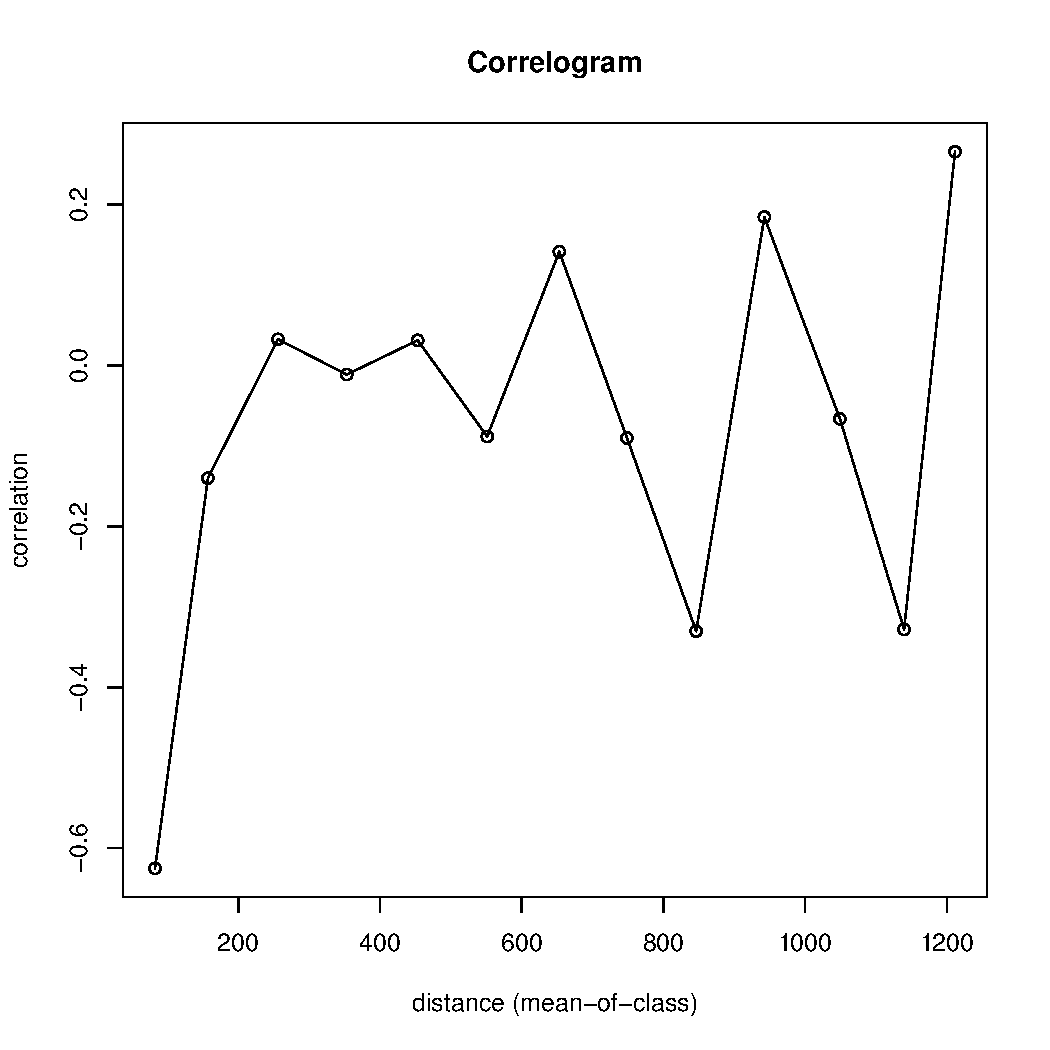
\includegraphics[width=80mm]{../Barenc_Sea/distribution_Moran/Yarnyshnaya07_moran_N_Macoma_balthica_.pdf}
	\end{center}
	\end{minipage}
%
	\hfil %Это пружинка отодвигающая рисунки друг от друга
%
	\begin{minipage}[b]{.46\linewidth}
%Следующий рисунок - первый ряд справа %DUNGEON S_4 \ AB
	\begin{center}
	{\small B}\\
		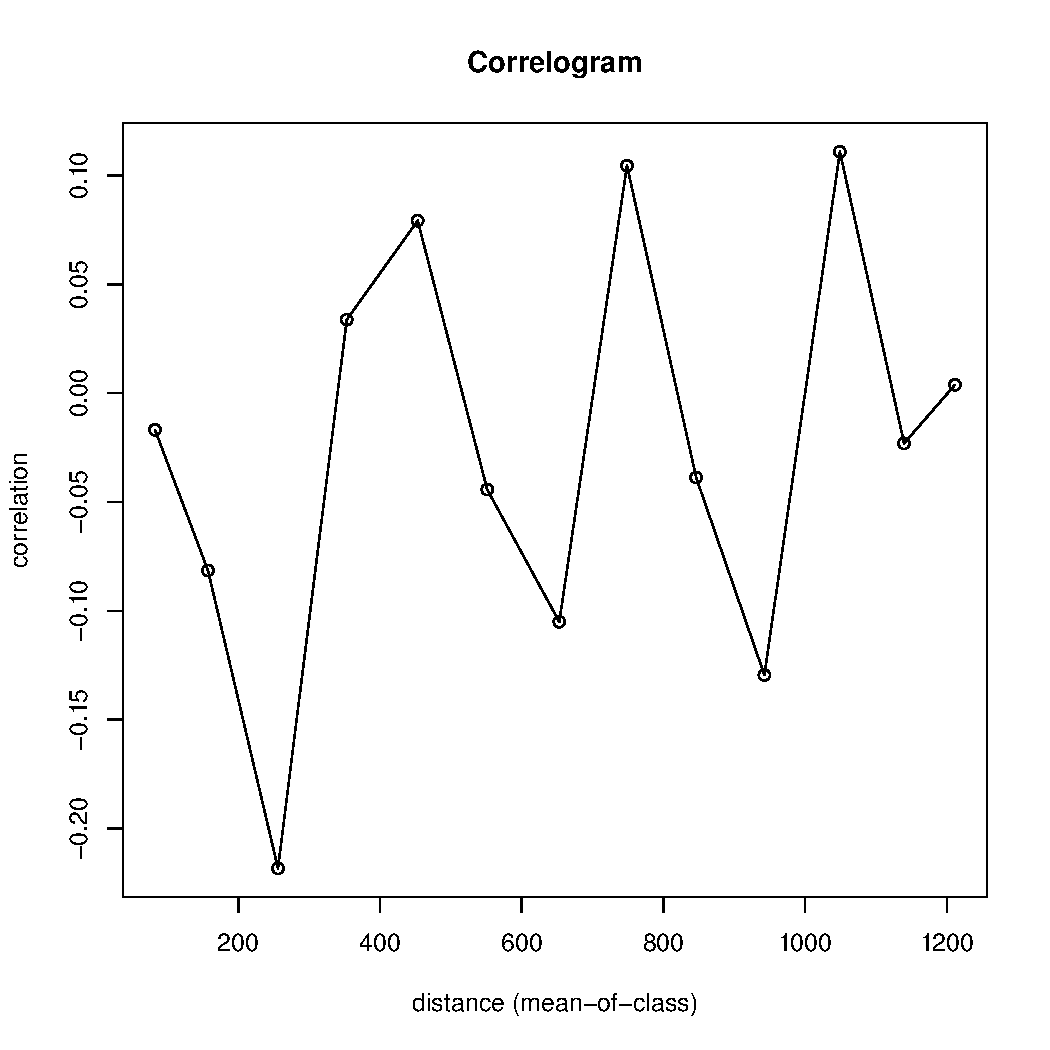
\includegraphics[width=80mm]{../Barenc_Sea/distribution_Moran/Yarnyshnaya07_moran_B_Macoma_balthica_.pdf}
	\end{center}
	\end{minipage}
	
	\begin{minipage}[b]{.46\linewidth}
	%Фигурка в первом ряду слева размер отведенный под весь этот объект -- 0.46 от ширины строки
	%Параметр [b] означает, что выравнивание этих министраниц будет по нижнему краю
	\begin{center}
		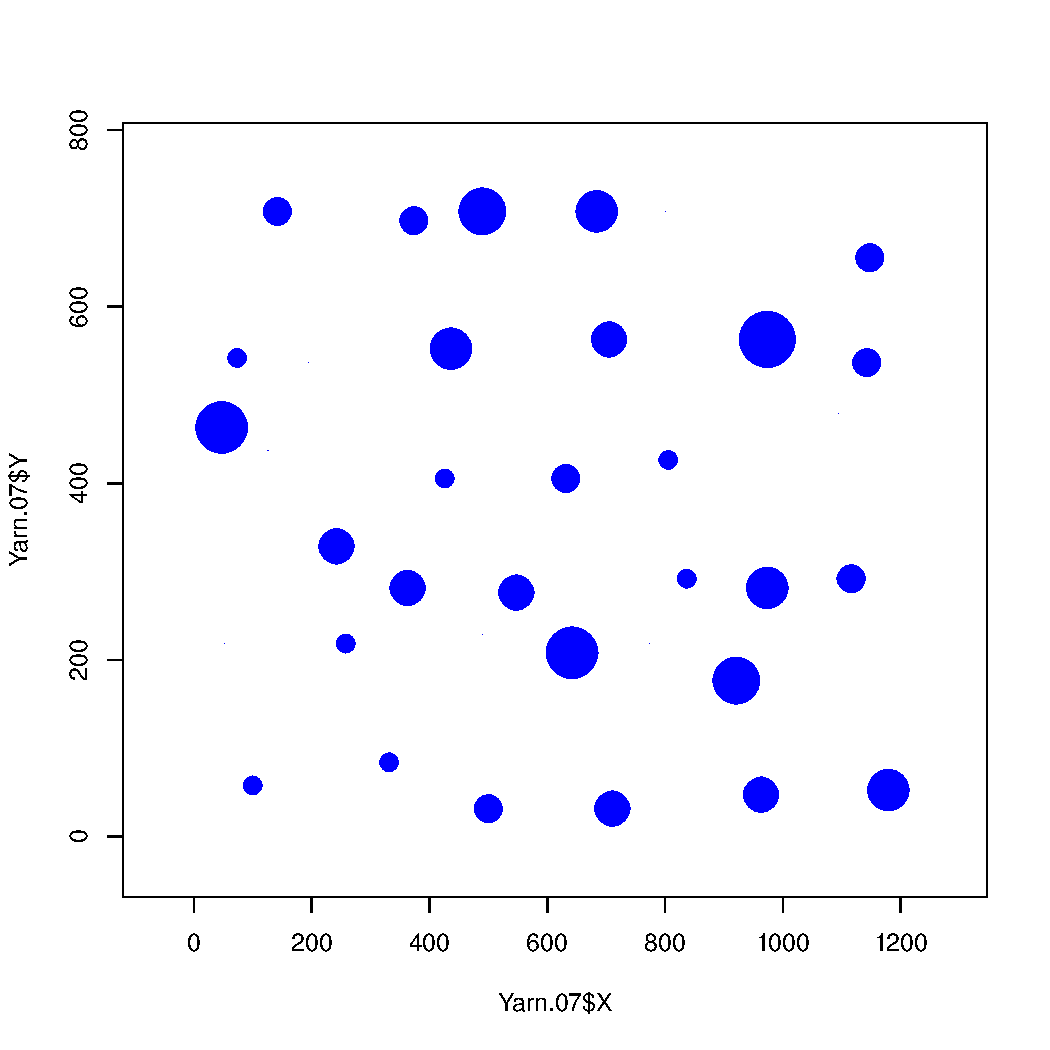
\includegraphics[width=80mm]{../Barenc_Sea/distribution_Moran/Yarnyshnaya_N_Macoma_bubbles.pdf}
	\end{center}
	\end{minipage}
	%
	\hfil %Это пружинка отодвигающая рисунки друг от друга
	%
	\begin{minipage}[b]{.46\linewidth}
%Следующий рисунок - первый ряд справа %DUNGEON S_4 \ AB
	\begin{center}
		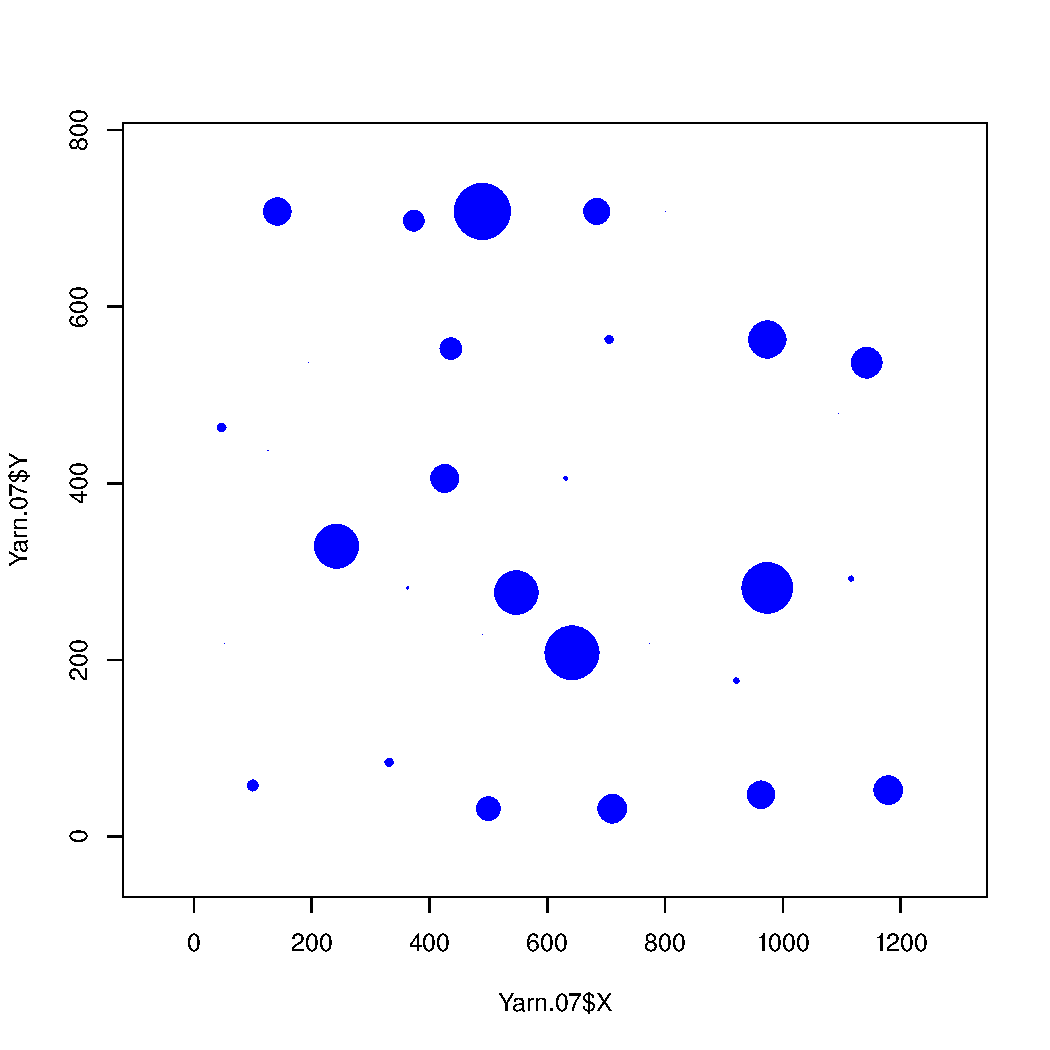
\includegraphics[width=80mm]{../Barenc_Sea/distribution_Moran/Yarnyshnaya_B_Macoma_bubbles.pdf}
	\end{center}
	\end{minipage}
	\caption{Коррелограммы Морана, описывающие микрораспределение, и реальное распределение {\it Macoma balthica} на литорали губы Ярнышная}
	\label{ris:MoranI_Yarnyshnaya}

	\footnotesize{Примечание: N --- распределение особей по численности. B -- распределение особей по биомассе.\\
	Moran's I --- коэффициент пространственной автокорреляции Морана. lag --- расстояние,~см. Закрашенные точки соответстсвуют достоверным значениям коэффициента корреляции ($p \le 0,05$).\\
	На пузырьковых диаграммах площадь кругов пропорциональна обилию маком.}
	\end{figure}



	\begin{figure}[h]

	\begin{minipage}[b]{.46\linewidth}
%Фигурка в первом ряду слева размер отведенный под весь этот объект -- 0.46 от ширины строки
%Параметр [b] означает, что выравнивание этих министраниц будет по нижнему краю
	\begin{center}
	{\small N}\\
		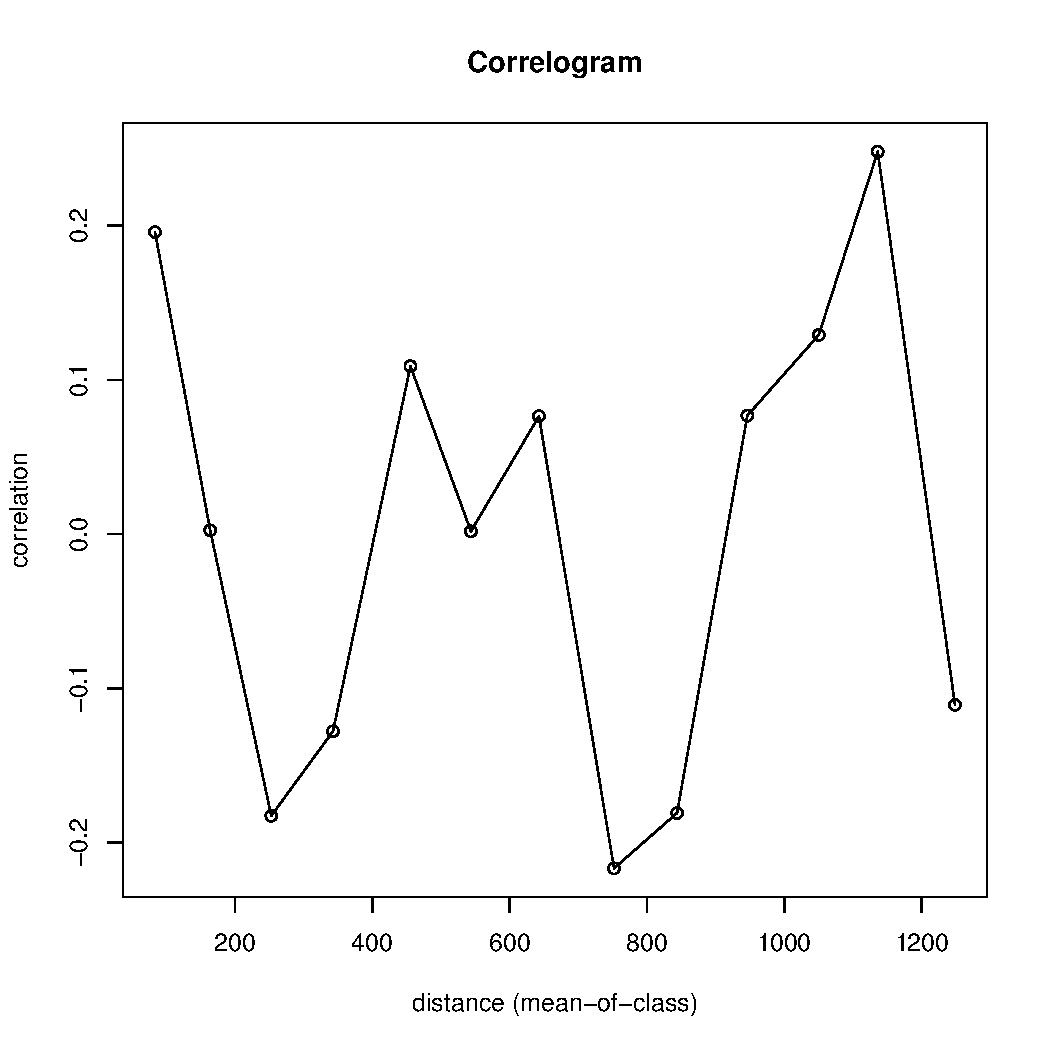
\includegraphics[width=80mm]{../Barenc_Sea/distribution_Moran/Plyazh07_moran_N_Macoma_balthica_.pdf}
	\end{center}
	\end{minipage}
%
	\hfil %Это пружинка отодвигающая рисунки друг от друга
%
	\begin{minipage}[b]{.46\linewidth}
%Следующий рисунок - первый ряд справа %DUNGEON S_4 \ AB
	\begin{center}
	{\small B}\\
		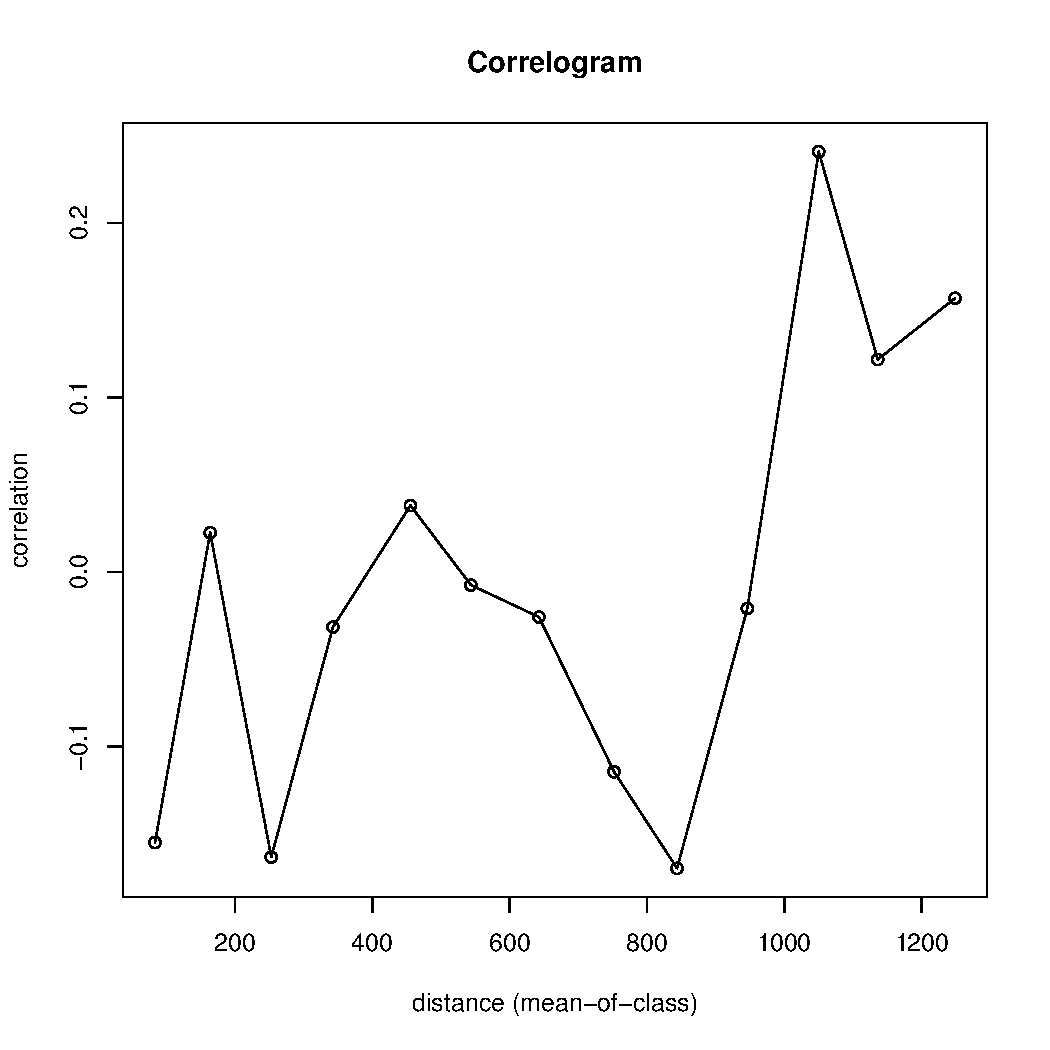
\includegraphics[width=80mm]{../Barenc_Sea/distribution_Moran/Plyazh07_moran_B_Macoma_balthica_.pdf}
	\end{center}
	\end{minipage}
	
	\begin{minipage}[b]{.46\linewidth}
	%Фигурка в первом ряду слева размер отведенный под весь этот объект -- 0.46 от ширины строки
	%Параметр [b] означает, что выравнивание этих министраниц будет по нижнему краю
	\begin{center}
		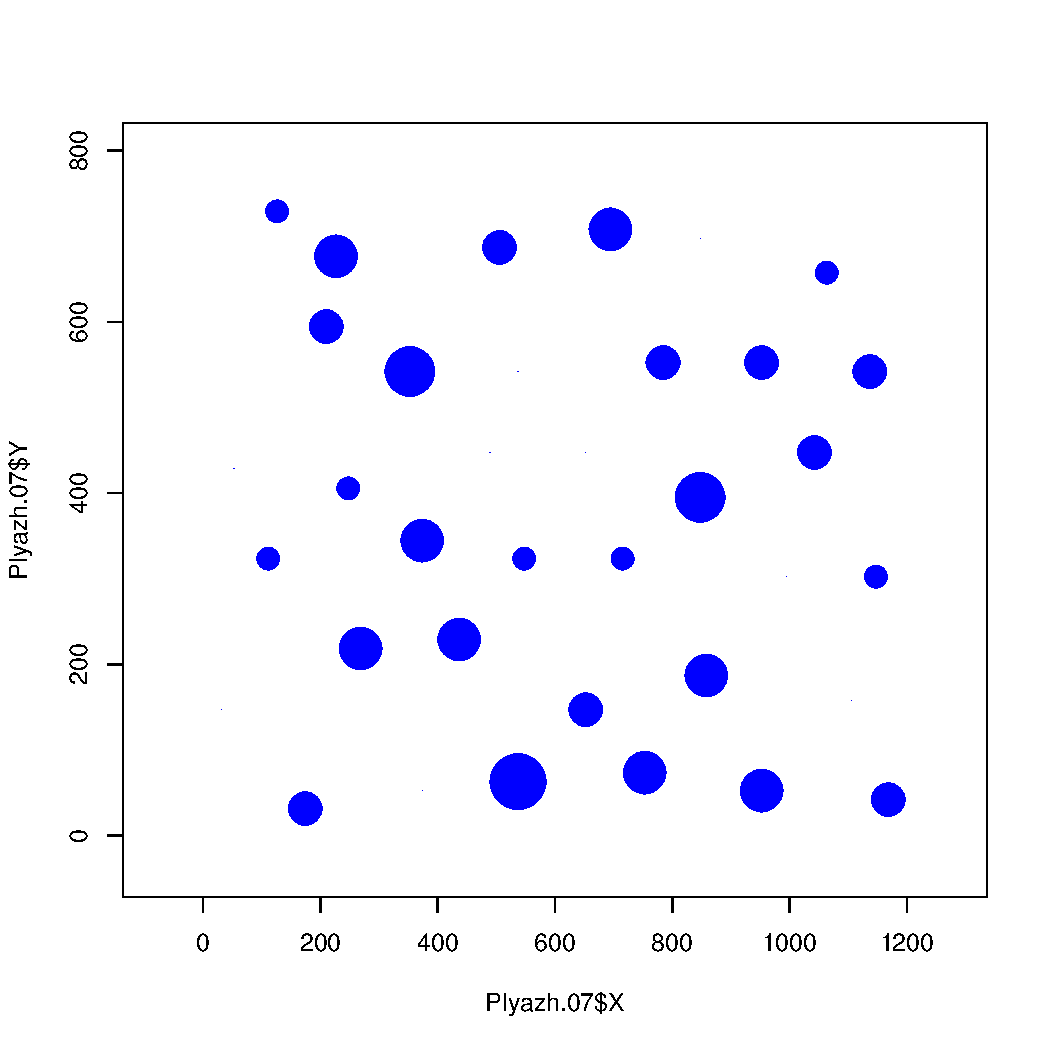
\includegraphics[width=80mm]{../Barenc_Sea/distribution_Moran/Plyazh07_N_Macoma_bubbles.pdf}
	\end{center}
	\end{minipage}
	%
	\hfil %Это пружинка отодвигающая рисунки друг от друга
	%
	\begin{minipage}[b]{.46\linewidth}
%Следующий рисунок - первый ряд справа %DUNGEON S_4 \ AB
	\begin{center}
		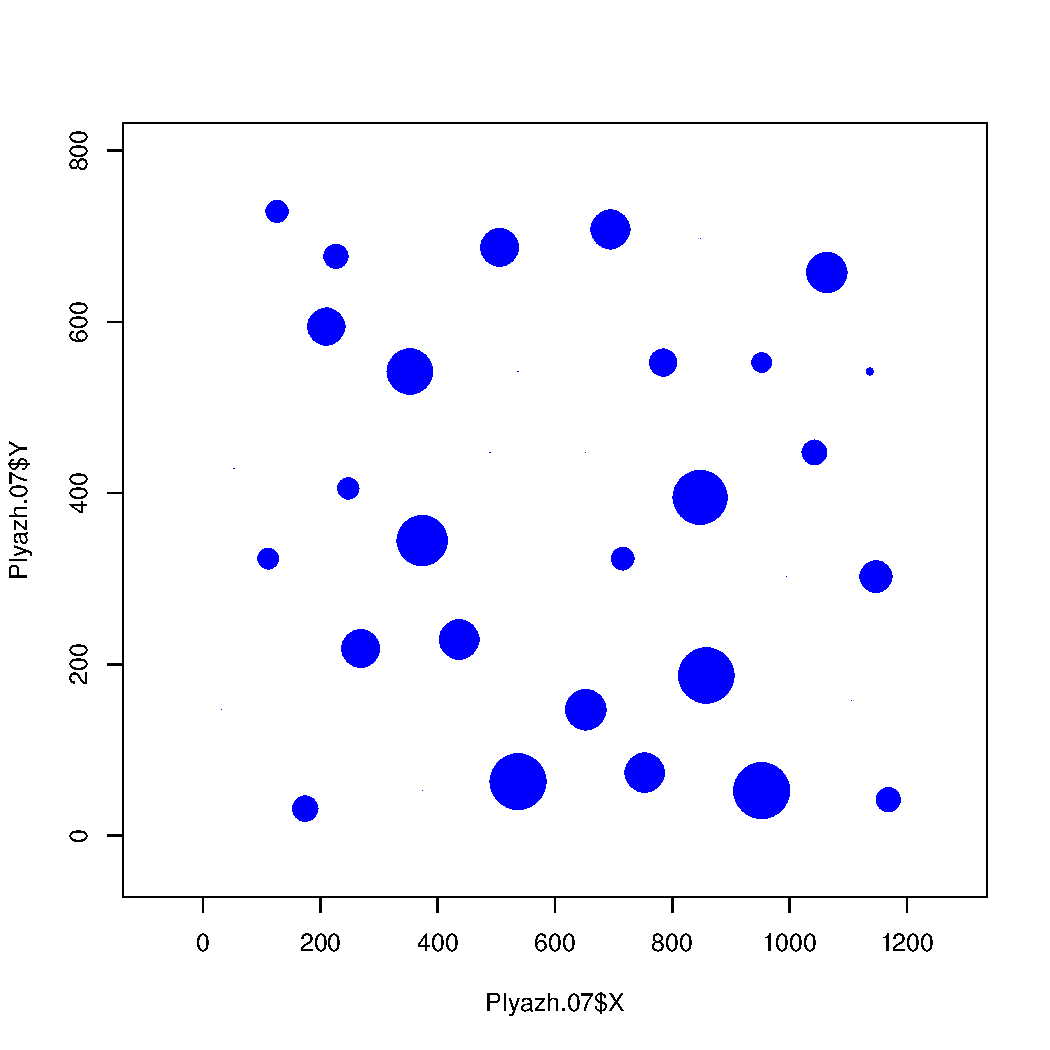
\includegraphics[width=80mm]{../Barenc_Sea/distribution_Moran/Plyazh07_B_Macoma_bubbles.pdf}
	\end{center}
	\end{minipage}
	\caption{Коррелограммы Морана, описывающие микрораспределение, и реальное распределение {\it Macoma balthica} на литорали губы Дальнезеленецкая в 2007 году}
	\label{ris:MoranI_DZ_2007}

	\footnotesize{Примечание: N --- распределение особей по численности. B -- распределение особей по биомассе.\\
	Moran's I --- коэффициент пространственной автокорреляции Морана. lag --- расстояние,~см. Закрашенные точки соответстсвуют достоверным значениям коэффициента корреляции ($p \le 0,05$).\\
	На пузырьковых диаграммах площадь кругов пропорциональна обилию маком.}
	\end{figure}

Мы предположили, что размер учетного полигона слишком маленький для выявления особенностей распределения, и в 2008 году повторили съемку, увеличив размер полигона и количество проб в два раза.
Достоверные значения коэффициента простарнственной корреляции Морана были показаны для расстояний около $1,5-2$~м (отрицательный) и на расстоянии около $4$~м (положительный) (рис.~\ref{ris:MoranI_DZ_2008}).
%
	\begin{figure}[h]

	\begin{minipage}[b]{.46\linewidth}
%Фигурка в первом ряду слева размер отведенный под весь этот объект -- 0.46 от ширины строки
%Параметр [b] означает, что выравнивание этих министраниц будет по нижнему краю
	\begin{center}
	{\small N}\\
		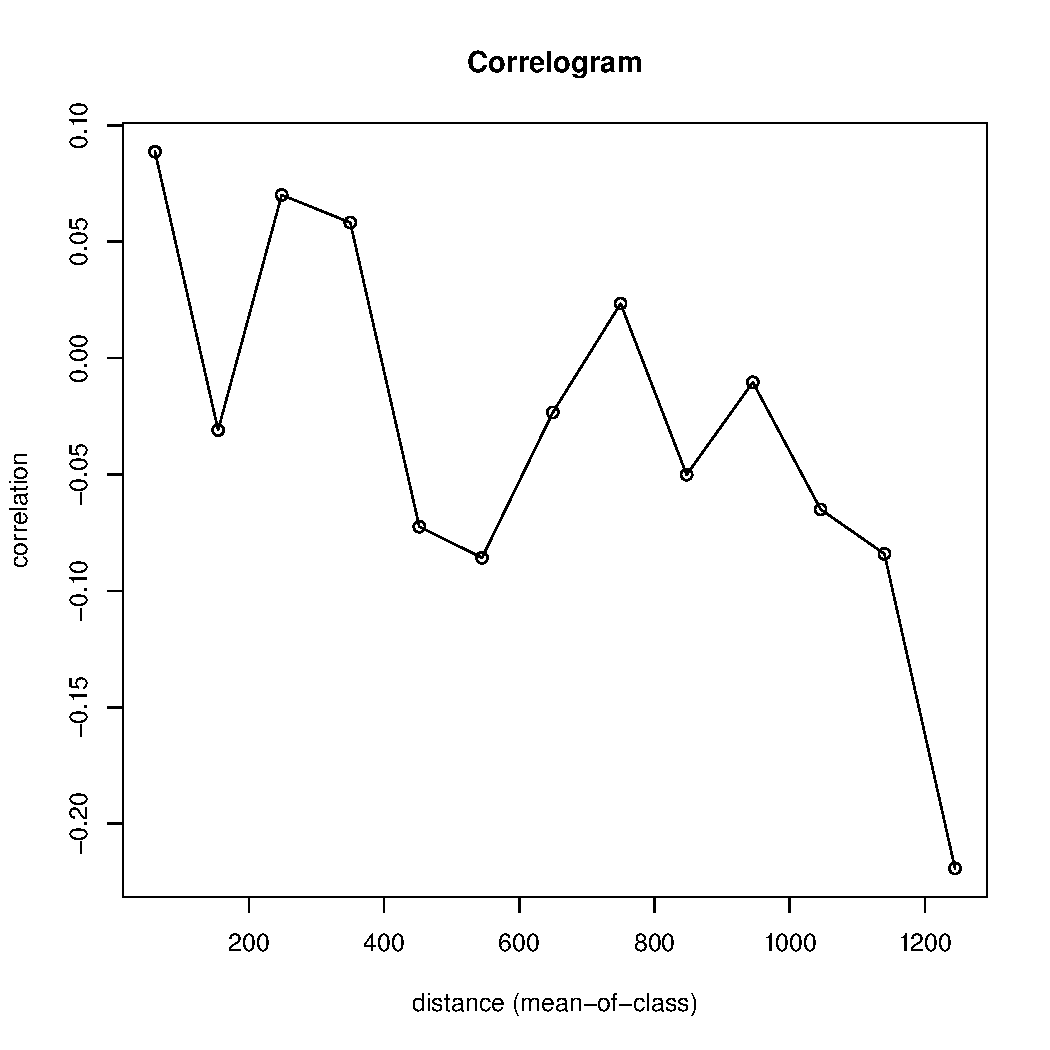
\includegraphics[width=80mm]{../Barenc_Sea/distribution_Moran/Plyazh0812_moran_N_Macoma_balthica_.pdf}
	\end{center}
	\end{minipage}
%
	\hfil %Это пружинка отодвигающая рисунки друг от друга
%
	\begin{minipage}[b]{.46\linewidth}
%Следующий рисунок - первый ряд справа %DUNGEON S_4 \ AB
	\begin{center}
	{\small B}\\
		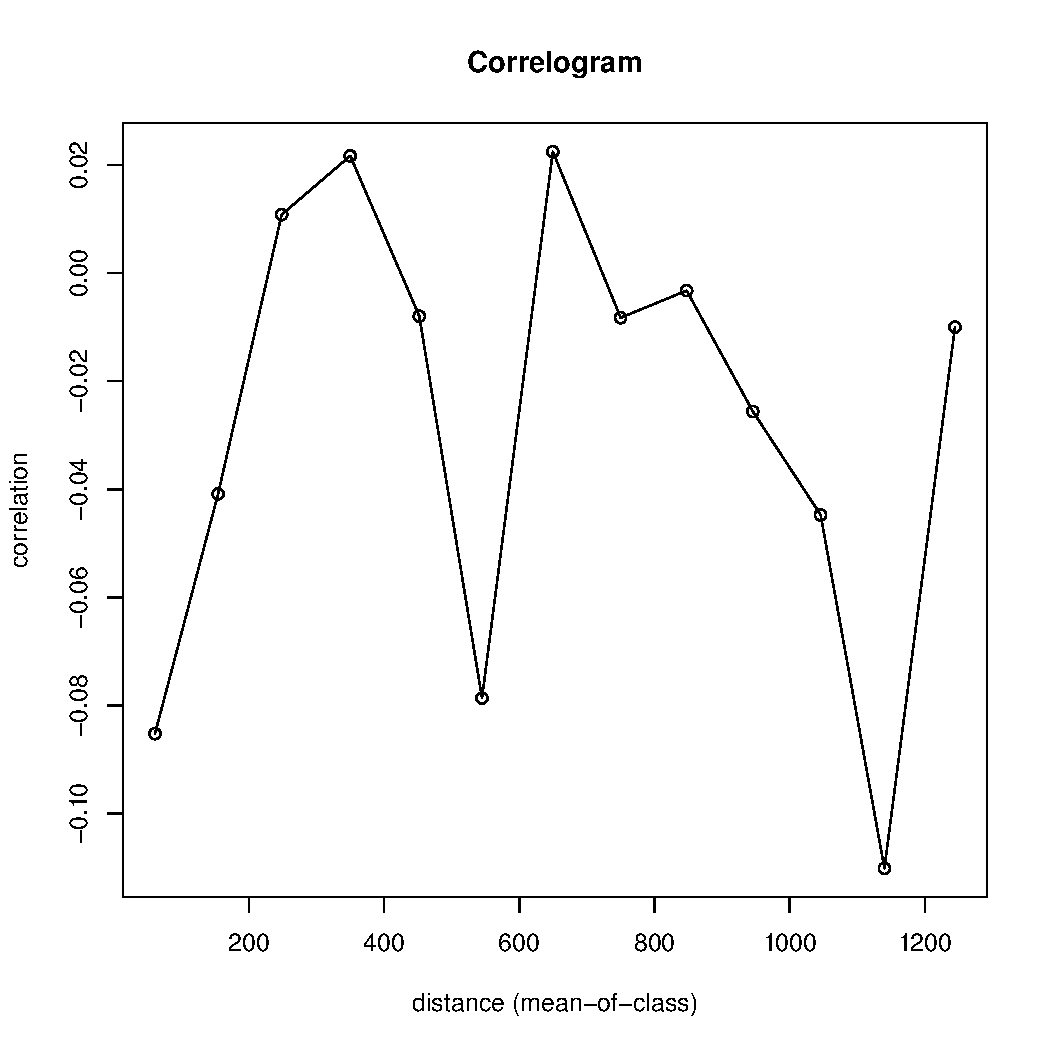
\includegraphics[width=80mm]{../Barenc_Sea/distribution_Moran/Plyazh0812_moran_B_Macoma_balthica_.pdf}
	\end{center}
	\end{minipage}
	
	\begin{minipage}[b]{.46\linewidth}
	%Фигурка в первом ряду слева размер отведенный под весь этот объект -- 0.46 от ширины строки
	%Параметр [b] означает, что выравнивание этих министраниц будет по нижнему краю
	\begin{center}
		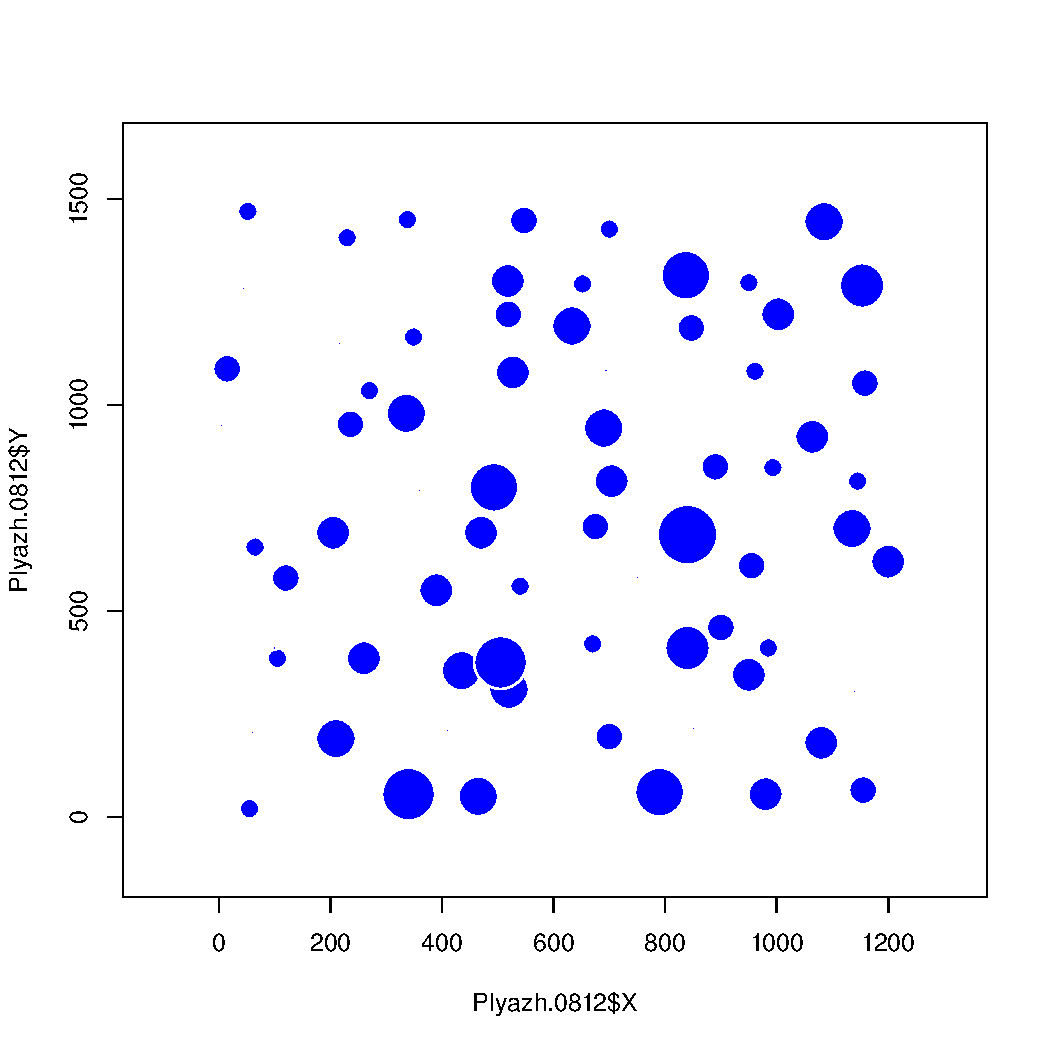
\includegraphics[width=80mm]{../Barenc_Sea/distribution_Moran/Plyazh0812_N_Macoma_bubbles.pdf}
	\end{center}
	\end{minipage}
	%
	\hfil %Это пружинка отодвигающая рисунки друг от друга
	%
	\begin{minipage}[b]{.46\linewidth}
%Следующий рисунок - первый ряд справа %DUNGEON S_4 \ AB
	\begin{center}
		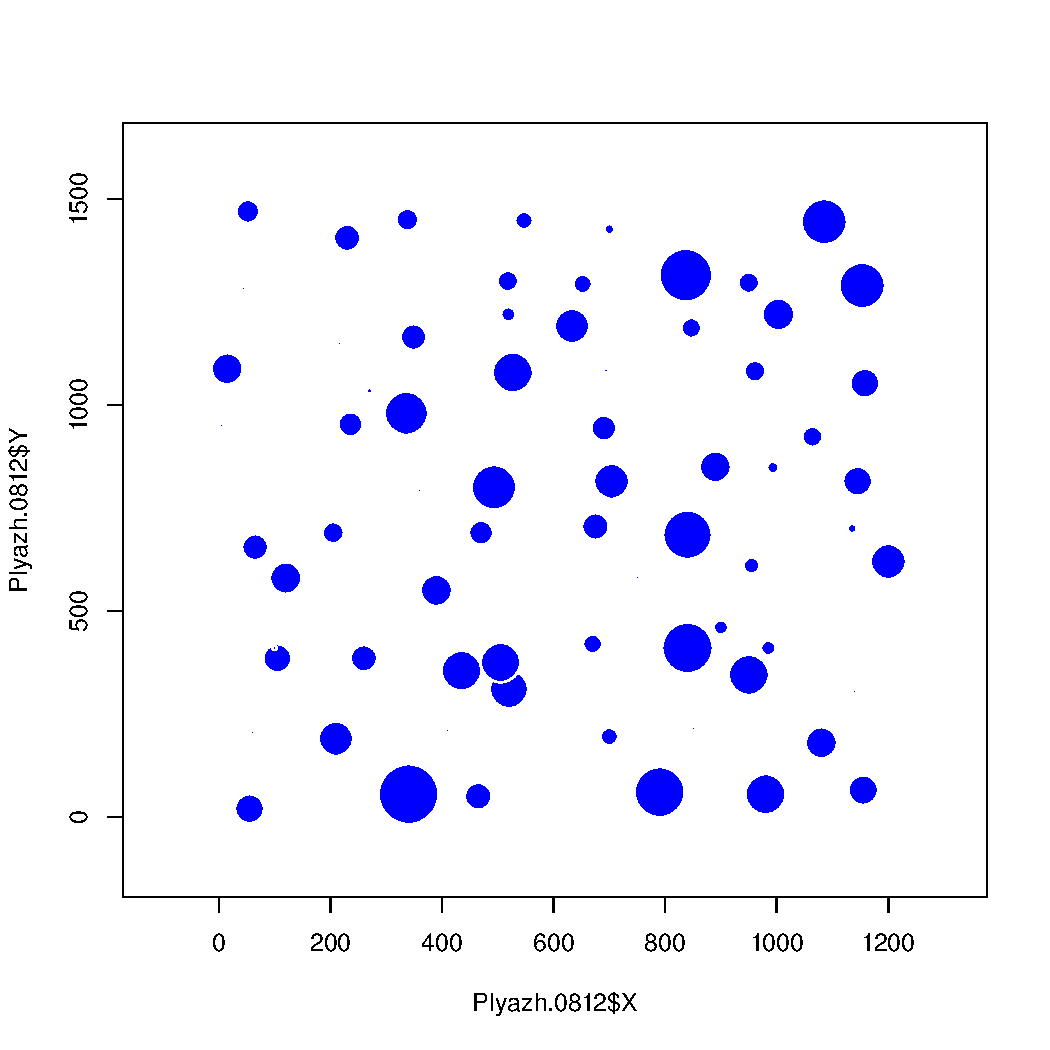
\includegraphics[width=80mm]{../Barenc_Sea/distribution_Moran/Plyazh0812_B_Macoma_bubbles.pdf}
	\end{center}
	\end{minipage}
	\caption{Коррелограммы Морана, описывающие микрораспределение, и реальное распределение {\it Macoma balthica} на литорали губы Дальнезеленецкая в 2008 году}
	\label{ris:MoranI_DZ_2008}

	\footnotesize{Примечание: N --- распределение особей по численности. B -- распределение особей по биомассе.\\
	Moran's I --- коэффициент пространственной автокорреляции Морана. lag --- расстояние,~см. Закрашенные точки соответстсвуют достоверным значениям коэффициента корреляции ($p \le 0,05$).\\
	На пузырьковых диаграммах площадь кругов пропорциональна обилию маком.}
	\end{figure}
%
Это позволяет предположить сложную структуру пространственного распределения особей: локальные агрегации, сравнимые по размеру с размером учетной рамки (1/30 м$^2$), организованные в более крупные скопления. 


	\subsection{Кольский залив}
На литорали Пала-губы особи {\it M.~balthica} формируют скопления размером около $2-4$~м (рис.~\ref{ris:moransI_Pala_Macoma}). 
Наличие серии достоверно отрицательных значений индекса автокорреляции Морана для больших расстояний свидетельствует о наличии либо градиентого изменения численности, либо крупной агрегации с нечеткими краями.
Наличие градиентного изменения обилия в направлении к руслу ручья было показано с использованием коэффициента корреляции Кендалла ($\tau = 0,55; p = 3,48 \times 10^{-6}$).
Распределение маком по биомассе соответствует распределению по численности (рис.~\ref{ris:moransI_Pala_Macoma}). Также корреляционный анализ Кендалла показал градиентное уменьшение биомассы в направлении от моря ($\tau = -0,4; p = 0,0005$).
	\begin{figure}[h]

	\begin{minipage}[b]{.5\linewidth}
	%Фигурка в первом ряду слева размер отведенный под весь этот объект -- 0.46 от ширины строки
	%Параметр [b] означает, что выравнивание этих министраниц будет по нижнему краю
	\begin{center}
	{\small N}\\
		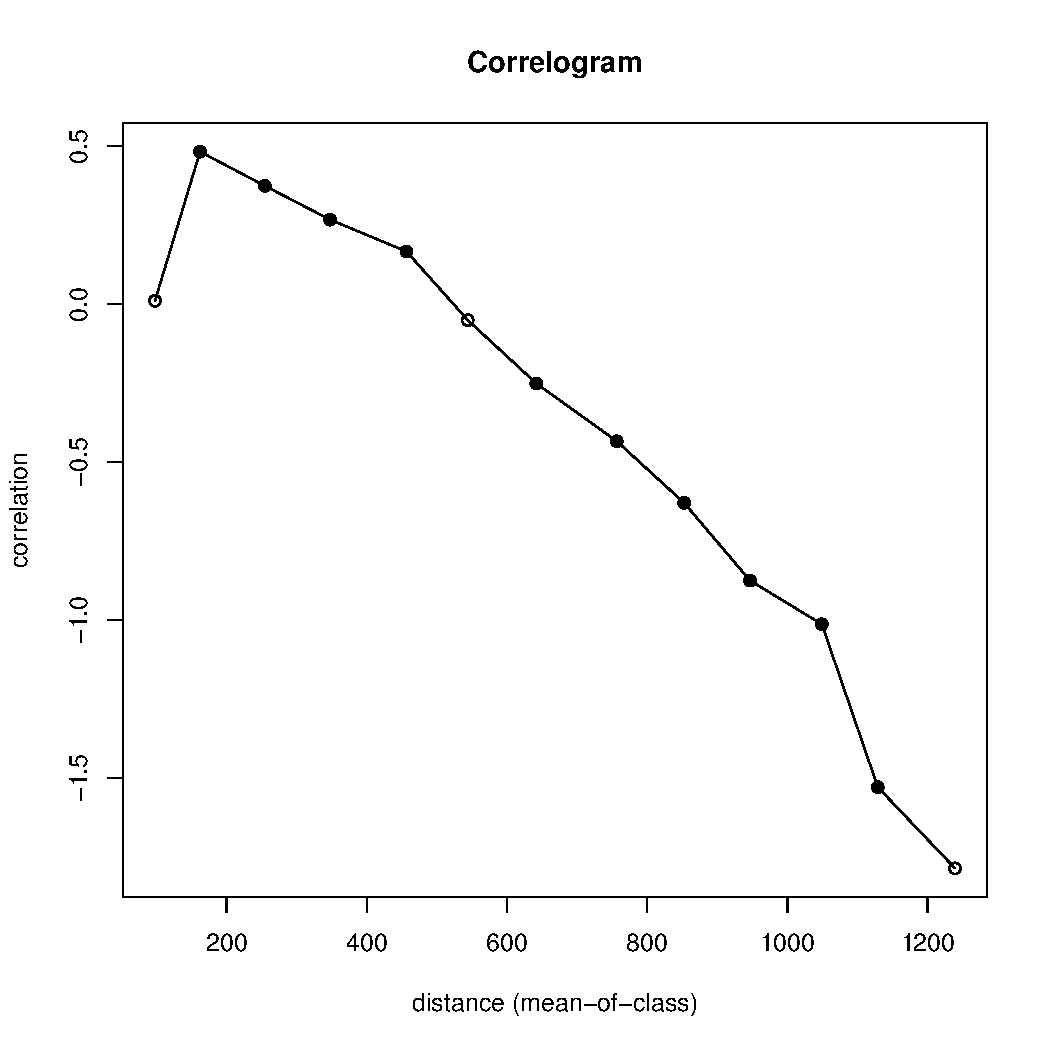
\includegraphics[width=80mm]{../Barenc_Sea/distribution_Moran/Pala_moran_N_Macoma_balthica_.pdf}
	\end{center}
	\end{minipage}
	%
	\hfil %Это пружинка отодвигающая рисунки друг от друга
	%
	\begin{minipage}[b]{.5\linewidth}
	%Следующий рисунок - первый ряд справа %DUNGEON S_4 \ AB
	\begin{center}
	{\small B}\\
		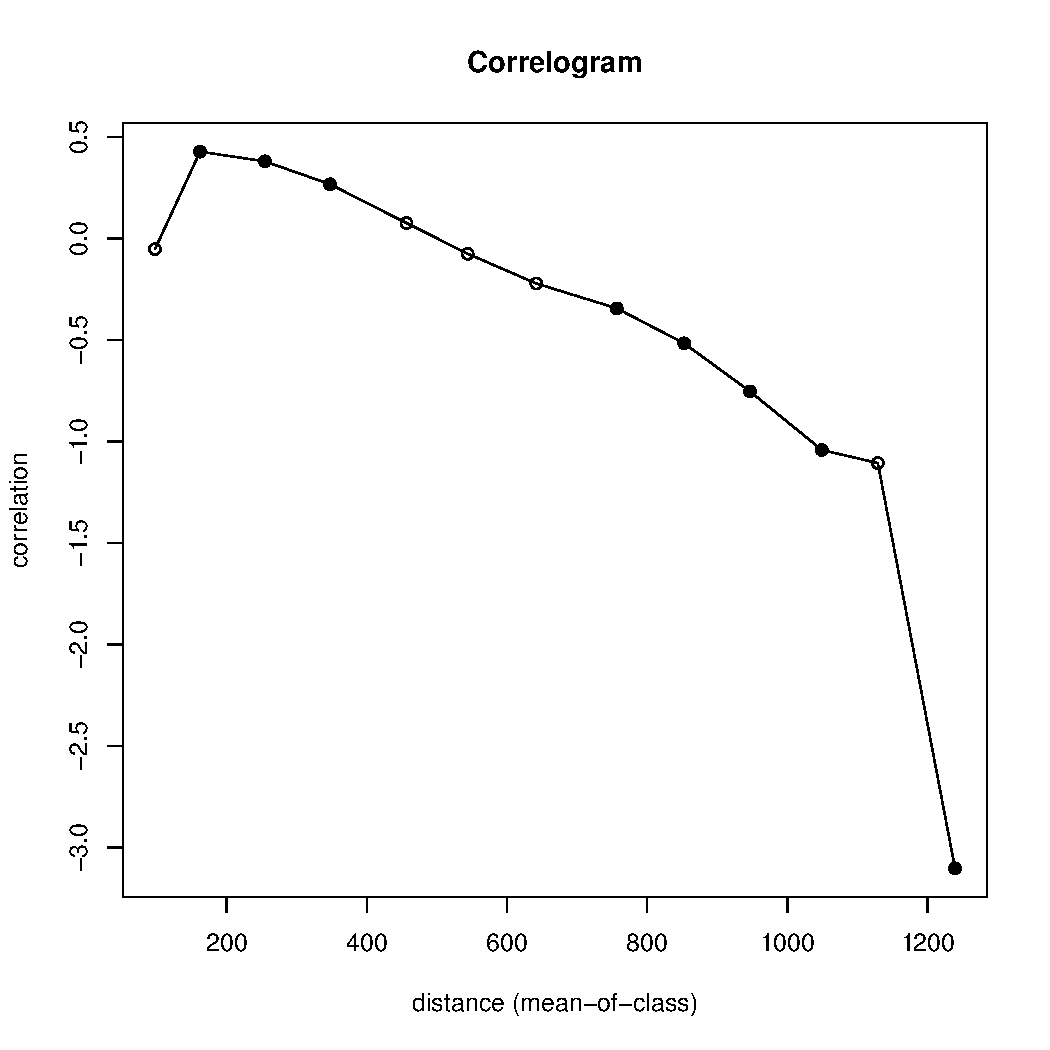
\includegraphics[width=80mm]{../Barenc_Sea/distribution_Moran/Pala_moran_B_Macoma_balthica_.pdf}
	\end{center}
	\end{minipage}

	\begin{minipage}[b]{.5\linewidth}
	\begin{center}
		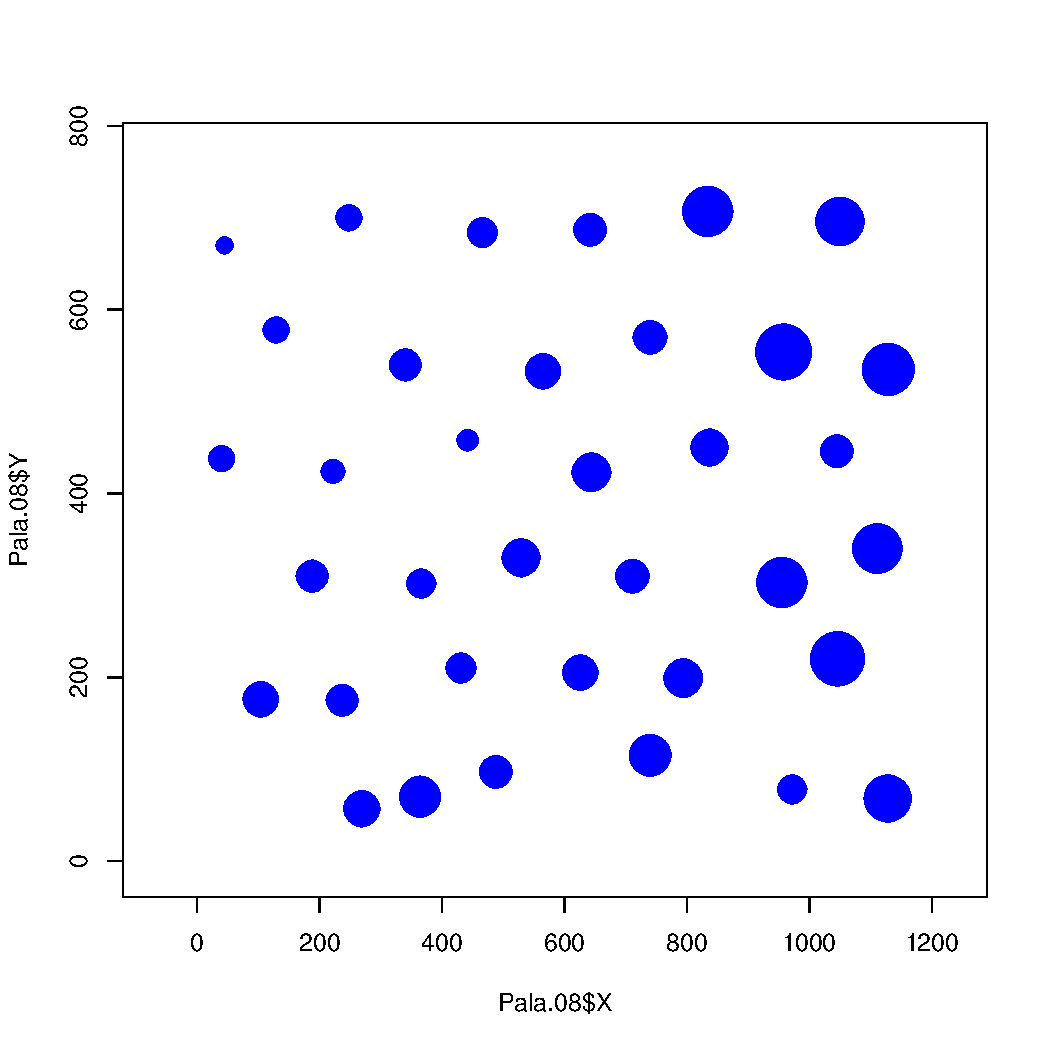
\includegraphics[width=80mm]{../Barenc_Sea/distribution_Moran/Pala_N_Macoma_bubbles.pdf}
	\end{center}
	\end{minipage}
	%
	\hfil %Это пружинка отодвигающая рисунки друг от друга
	%
	\begin{minipage}[b]{.5\linewidth}
	%Следующий рисунок - первый ряд справа %DUNGEON S_4 \ AB
	\begin{center}
		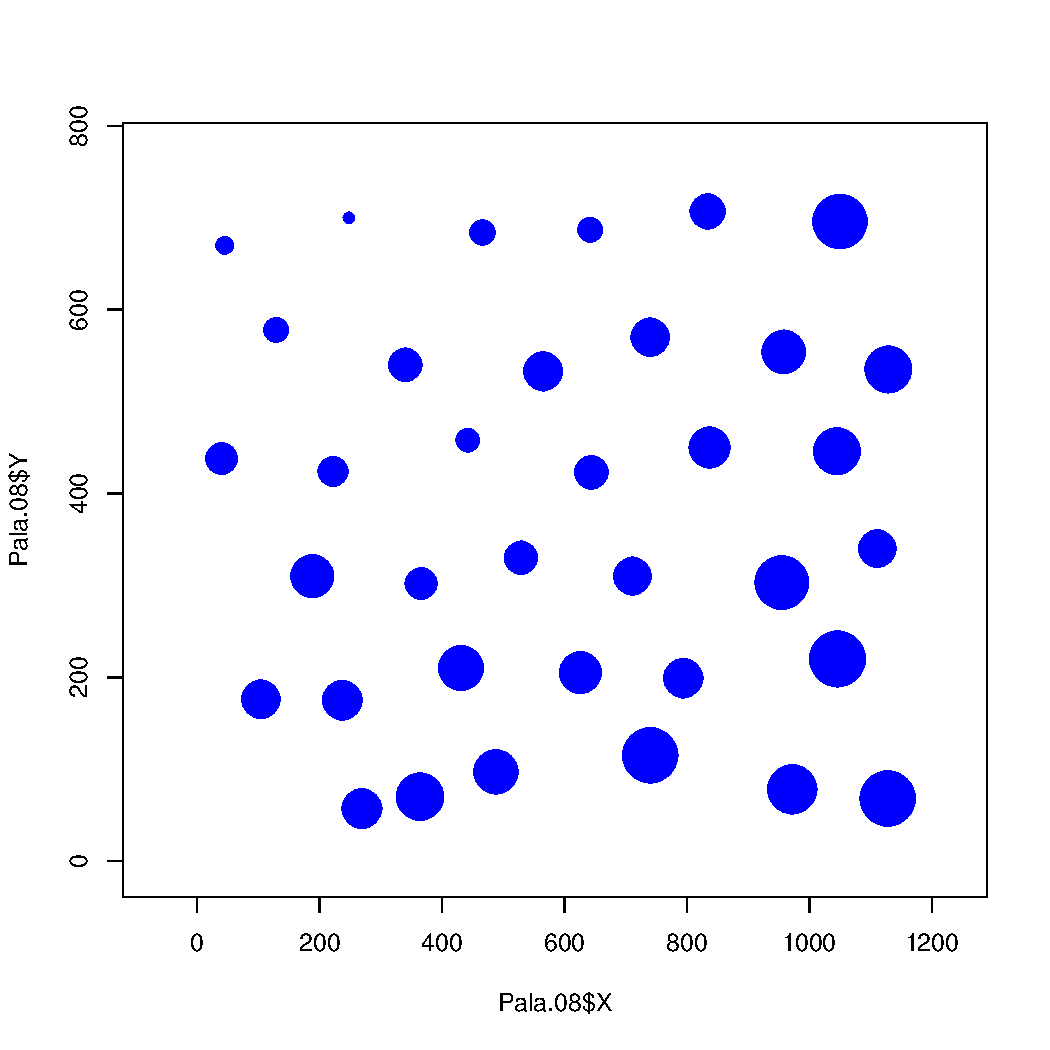
\includegraphics[width=80mm]{../Barenc_Sea/distribution_Moran/Pala_B_Macoma_bubbles.pdf}
	\end{center}
	\end{minipage}
	\caption{Коррелограммы Морана, описывающие микрораспределение, и реальное распределение {\it Macoma balthica} на литорали Пала-губы}
	\label{ris:moransI_Pala_Macoma}

	\footnotesize{Примечание: N --- распределение особей по численности. B -- распределение особей по биомассе.\\
	Moran's I --- коэффициент пространственной автокорреляции Морана. lag --- расстояние,~см. Закрашенные точки соответстсвуют достоверным значениям коэффициента корреляции ($p \le 0,05$).\\
	На пузырьковых диаграммах площадь кругов пропорциональна обилию маком.}
	\end{figure}

Поскольку на данном участке обилие маком было достаточно высокое (рис.~\ref{ris:age_Pala_2007_low}), мы отдельно рассмотрели распределение особей разных возрастов.
%
	\begin{figure}[h]
		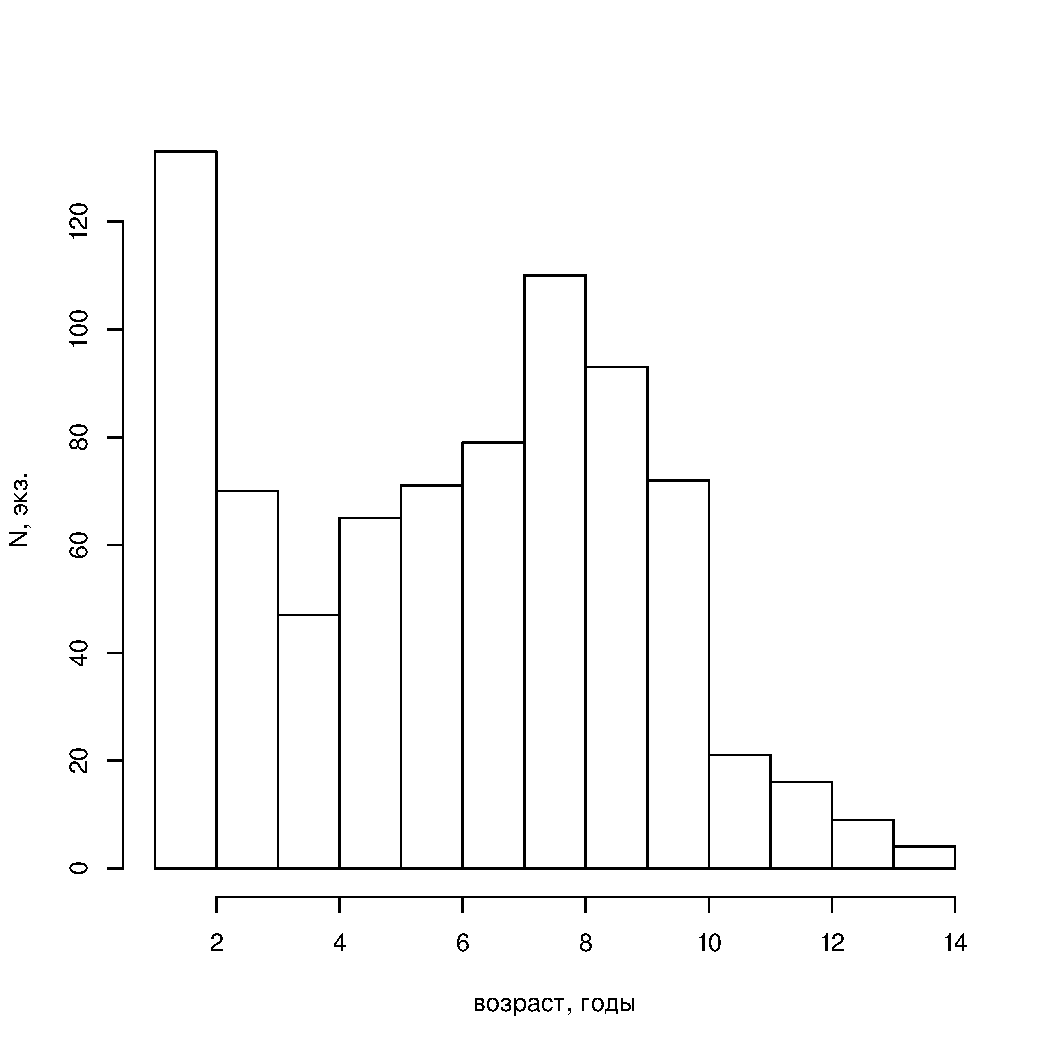
\includegraphics{../Barenc_Sea/Pala/Pala_2007_low_age_hist.pdf}
		\caption{Распределение по возрастам особей {\it Macoma balthica} в пробах на литорали Пала-губы}
		\label{ris:age_Pala_2007_low}
	\end{figure}
%
Коррелограммы Морана и пузырьковые диаграммы, описывающие реальное распределение особей, представлены в приложении \ref{app:Pala_MoranI_ages}.
Было показано, что горизонтальный градиент общего обилия связан в первую очередь с таким распределением особей возрастом 2, 3 и 5 лет (табл.~\ref{tab:Pala_ages_distribution}). 
%
\begin{table}[h]
		\caption{Пространственное распределение особей {\it Macoma balthica} разного возраста}
		\label{tab:Pala_ages_distribution}
\begin{tabularx}{\linewidth}{|c|X|rr|rr|}
\hline
	& распределение		& \multicolumn{2}{c|}{градиент горизонтальный} & \multicolumn{2}{c|}{градиент вертикальный}   \\ \cline{3-6}
возраст  &  по результатам пространственной автокорреляции  & $Kendall\ \tau$ & $p-value$ & $Kendall\ \tau$ & $p-value$				\\ \hline

1+       & случайное                      & $0,2$	&	$0,17$	&	$0,02$	&	$0,9$                            \\
2+       & градиент                       & $0,45$	&	$0,0003$ ***	&	$0,2$	&	$0,07$ **                   \\
3+       & градиент                       & $0,5$	&	$2,4 \times 10^{-5}$ ***	&	$0,3$	&	$0,002$ ***		 \\
4+       & случайное                      & $0,2$	&	$0,07$ **	&	$0,06$	&	$0,6$                            \\
5+       & градиент                       & $0,43$	&	$0,0005$ ***	&	$-0,02$	&	$0,9$                    \\
6+       & случайное                      & $0,2$	&	$0,03$ ***	&	$-0,03$	&	$0,8$                            \\
7+       & одно большое пятно             & $0,02$	&	$0,9$	&	$-0,02$	&	$0,9$                             \\
8+       & одно большое пятно             & $0,3$	&	$0,01$ ***	&	$-0,2$	&	$0,04$ ***                            \\
9+       & одно большое пятно             & $0,3$	&	$0,01$ ***	&	$-0,2$	&	$0,1$                             \\
10+      & агрегации размером 1 и 3 метра & $0,2$	&	$0,1$	&	$-0,2$	&	$0,08$ **                            \\
11+      & одно большое пятно             & $0,26$	&	$0,053$ **	&	$-0,1$	&	$0,3$                             \\
12+      & агрегации размером 6 метров    & $0,1$	&	$0,3$	&	$-0,2$	&	$0,2$                             \\
13+      & случайное                      & $0,1$	&	$0,4$	&	$0,04$	&	$0,7$                              \\
14+      & случайное                      &  $0,09$	&	$0,5$	&	$-0,15$	&	$0,3$                             \\ \hline
	\end{tabularx}
\end{table}
%
Предположения о градиентном распределении особей данных возрастов, полученных в ходе анализа пространственных автокорреляций Морана подтвердились при корреляционном анализе Кендалла (табл.~\ref{tab:Pala_ages_distribution}).
Однако в нескольких случаях, где коррелограммы Морана не показывают градиентного распределения, анализ Кендалла показывает достоверную корреляцию обилия с координатами. 
Однако во всех случаях речь идет о слабой связи (коэффициент корреляции $0,2$).

Резюмируя полученные данные, можно говорить о большем влиянии ручья на более молодых моллюсков.
Особи старших возрастов формируют агрегации размером в несколько метров.
Наиболее старые моллюски остаются в количестве единичных особей и распределены случайно.



%%популяционная структура

	\section{Численность {\it Macoma balthica}}
	\subsection{Белое море}
Данные по обилию маком в Кандалакшском заливе Белого моря получены для $10$ участков, всего 140 пространственно-временных точек оценки.
Средняя численность {\it M.~balthica} была представлена в диапазоне от $10$ (о.~Горелый) до $8500$~экз./м$^2$(Западная Ряшкова салма) (табл. \ref{tab:mean_N_White}).
	\begin{footnotesize}
	\begin{longtable}{|p{2cm}|p{3cm}|p{1cm}|p{2cm}|p{1.5cm}|p{1cm}|*{3}{c|}}
	\caption{Средняя численность {\it Macoma balthica} на различных участках Белого моря}\label{tab:mean_N_White}\\
	\hline
	Район & Участок & год & ма\-ре\-ографи\-ческий уровень & число повторностей & площадь учета & $N$, экз./м$^2$ & $S_x$  & $D, \%$ 
	\\ \hline \endfirsthead
	\hline
	\multicolumn{9}{|c|}{продолжение таблицы \ref{tab:mean_N_White}} \\ \hline
	Район & Участок & год & ма\-ре\-ографи\-ческий уровень & число повторностей & площадь учета & $N$, экз./м$^2$ & $S_x$  & $D, \%$ 
	\\ \hline \endhead
	\hline 
	\multicolumn{9}{|c|}{продолжение таблицы \ref{tab:mean_N_White} на следующей странице}
	\\ \hline \endfoot
	 \endlastfoot
	г. Чупа & б. Клющиха & 2006 & СГЛ & 10 & 1/20 & 444 & 53,7 & 12
		\\ \cline{3-9}
		 &  & 2006 & НГЛ & 10 & 1/20 & 362 & 26,4 & 7
		\\ \cline{3-9}
		 &  & 2006 & ВСЛ & 10 & 1/20 & 1136 & 55,4 & 5
		\\ \cline{2-9}
		 & Сухая салма & 2006 & СГЛ & 10 и & 2/20 & 1165 & 169,3 & 15
		\\ \cline{3-9}
		 &  & 2006 & НГЛ & 5 & 1/20 & 1132 & 82,6 & 7
		\\ \cline{3-9}
		 &  & 2006 & НГЛ, пояс зостеры & 5 & 1/20 & 992 & 174,4 & 18
		\\ \cline{2-9}
		 & б. Лисья & 2006 & СГЛ & 10 & 1/20 & 1346 & 209,8 & 16
		\\ \cline{3-9}
		 &  & 2006 & НГЛ & 10 & 1/20 & 2832 & 277,8 & 10
		\\ \cline{3-9}
		 &  & 2006 & ВСЛ & 10 & 1/20 & 1006 & 159,8 & 16
		\\ \cline{2-9}
		 & пр. Подпахта & 2006 & СГЛ & 10 & 1/20 & 688 & 145,2 & 21
		\\ \cline{3-9}
		 &  & 2006 & НГЛ & 10 & 1/20 & 372 & 57,9 & 16
		\\ \hline
	Лувеньга & материковая литораль, Лувеньга & 1992 & верхний пляж & 7 & 1/30 & 94 & 35,5 & 38
		\\ \cline{4-9}
		 &  & 1992 & пояс фукоидов & 5 & 1/30 & 114 & 55,6 & 49
		\\ \cline{4-9}
		 &  &  & пояс зостеры & 5 & 1/30 & 222 & 103,3 & 47
		\\ \cline{4-9}
		 &  &  & нижний пляж & 3 & 1/30 & 560 & 457,1 & 82
		\\ \cline{3-9}
		 &  & 1993 & верхний пляж & 4 & 1/30 & 413 & 127,5 & 31
		\\ \cline{4-9}
		 &  &  & пояс фукоидов & 5 & 1/30 & 336 & 120,9 & 36
		\\ \cline{4-9}
		 &  &  & пояс зостеры & 6 & 1/30 & 405 & 80,0 & 20
		\\ \cline{4-9}
		 &  & & нижний пляж & 5 & 1/30 & 354 & 77,3 & 22
		\\ \cline{3-9}
		 &  & 1994 & верхний пляж & 5 & 1/30 & 462 & 179,1 & 39
		\\ \cline{4-9}
		 &  &  & пояс фукоидов & 6 & 1/30 & 745 & 220,6 & 30
		\\ \cline{4-9}
		 &  &  & пояс зостеры & 6 & 1/30 & 765 & 112,7 & 15
		\\ \cline{4-9}
		 &  &  & нижний пляж & 3 & 1/30 & 930 & 170,6 & 18
		\\ \cline{3-9}
		 &  & 1995 & верхний пляж & 4 & 1/30 & 908 & 222,3 & 24
		\\ \cline{4-9}
		 &  &  & пояс фукоидов & 5 & 1/30 & 1134 & 269,7 & 24
		\\ \cline{4-9}
		 &  &  & пояс зостеры & 5 & 1/30 & 660 & 117,7 & 18
		\\ \cline{4-9}
		 &  &  & нижний пляж & 6 & 1/30 & 685 & 154,8 & 23
		\\ \cline{3-9}
		 &  & 1996 & верхний пляж & 4 & 1/30 & 698 & 257,0 & 37
		\\ \cline{4-9}
		 &  &  & пояс фукоидов & 6 & 1/30 & 770 & 214,9 & 28
		\\ \cline{4-9}
		 &  &  & пояс зостеры & 4 & 1/30 & 645 & 71,9 & 11
		\\ \cline{4-9}
		 &  &  & нижний пляж & 6 & 1/30 & 870 & 68,8 & 8
		\\ \cline{3-9}
		 &  & 1997 & верхний пляж & 3 & 1/30 & 620 & 130,0 & 21
		\\ \cline{4-9}
		 &  &  & пояс фукоидов & 6 & 1/30 & 720 & 265,6 & 37
		\\ \cline{4-9}
		 &  &  & пояс зостеры & 5 & 1/30 & 702 & 70,7 & 10
		\\ \cline{4-9}
		 &  &  & нижний пляж & 6 & 1/30 & 880 & 97,0 & 11
		\\ \cline{3-9}
		 &  & 1998 & верхний пляж & 4 & 1/30 & 2130 & 623,9 & 29
		\\ \cline{4-9}
		 &  &  & пояс фукоидов & 6 & 1/30 & 2750 & 820,0 & 30
		\\ \cline{4-9}
		 &  &  & пояс зостеры & 5 & 1/30 & 2424 & 437,1 & 18
		\\ \cline{4-9}
		 &  &  & нижний пляж & 5 & 1/30 & 1182 & 239,0 & 20
		\\ \cline{3-9}
		 &  & 1999 & верхний пляж & 3 & 1/30 & 7240 & 5833,7 & 81
		\\ \cline{4-9}
		 &  &  & пояс фукоидов & 6 & 1/30 & 3895 & 1354,6 & 35
		\\ \cline{4-9}
		 &  &  & пояс зостеры & 6 & 1/30 & 2405 & 498,8 & 21
		\\ \cline{4-9}
		 &  &  & нижний пляж & 5 & 1/30 & 2328 & 623,8 & 27
		\\ \cline{3-9}
		 &  & 2000 & верхний пляж & 2 & 1/30 & 2640 & 870,0 & 33
		\\ \cline{4-9}
		 &  &  & пояс фукоидов & 4 & 1/30 & 2760 & 373,1 & 14
		\\ \cline{4-9}
		 &  & & пояс зостеры & 5 & 1/30 & 2562 & 721,0 & 28
		\\ \cline{4-9}
		 &  &  & нижний пляж & 4 & 1/30 & 2018 & 394,3 & 20
		\\ \cline{3-9}
		 &  & 2002 & верхний пляж & 3 & 1/30 & 1360 & 401,5 & 30
		\\ \cline{4-9}
		 &  &  & пояс фукоидов & 3 & 1/30 & 3250 & 337,8 & 10
		\\ \cline{4-9}
		 &  &  & пояс зостеры & 4 & 1/30 & 2498 & 952,6 & 38
		\\ \cline{4-9}
		 &  &  & нижний пляж & 2 & 1/30 & 810 & 240,0 & 30
		\\ \cline{3-9}
		 &  & 2004 & верхний пляж & 3 & 1/30 & 2800 & 1066,6 & 38
		\\ \cline{4-9}
		 &  &  & пояс фукоидов & 4 & 1/30 & 3090 & 889,0 & 29
		\\ \cline{4-9}
		 &  &  & пояс зостеры & 5 & 1/30 & 1818 & 302,6 & 17
		\\ \cline{2-9}
		 & о. Горелый & 1992 & ВГЛ & 7 & 1/30 & 73 & 23,7 & 32
		\\ \cline{4-9}
		 &  &  & СГЛ & 5 & 1/30 & 108 & 9,7 & 9
		\\ \cline{4-9}
		 &  &  & НГЛ & 2 & 1/30 & 50 & 20,0 & 40
		\\ \cline{4-9}
		 &  &  & ноль глубин & 3 & 1/30 & 13 & 3,3 & 25
		\\ \cline{3-9}
		 &  & 1993 & ВГЛ & 3 & 1/30 & 143 & 29,1 & 20
		\\ \cline{4-9}
		 &  &  & СГЛ & 3 & 1/30 & 480 & 11,5 & 2
		\\ \cline{4-9}
		 &  &  & НГЛ & 4 & 1/30 & 183 & 34,5 & 19
		\\ \cline{4-9}
		 &  &  & ноль глубин & 3 & 1/30 & 97 & 43,7 & 45
		\\ \cline{3-9}
		 &  & 2004 & ВГЛ & 3 & 1/30 & 2620 & 219,3 & 8
		\\ \cline{4-9}
		 &  &  & СГЛ & 3 & 1/30 & 1700 & 208,8 & 12
		\\ \cline{4-9}
		 &  &  & НГЛ & 3 & 1/30 & 1040 & 176,9 & 17
		\\ \cline{4-9}
		 &  &  & ноль глубин & 3 & 1/30 & 1540 & 60,8 & 4
		\\ \cline{3-9}
		 &  & 2006 & ВГЛ & 3 & 1/30 & 2200 & 353,4 & 16
		\\ \cline{4-9}
		 &  &  & СГЛ & 3 & 1/30 & 1910 & 342,2 & 18
		\\ \cline{4-9}
		 &  &  & НГЛ & 3 & 1/30 & 650 & 87,2 & 13
		\\ \cline{4-9}
		 &  &  & ноль глубин & 3 & 1/30 & 760 & 160,9 & 21
		\\ \cline{3-9}
		 &  & 2007 & ВГЛ & 3 & 1/30 & 1940 & 341,8 & 18
		\\ \cline{4-9}
		 &  &  & СГЛ & 3 & 1/30 & 1990 & 449,8 & 23
		\\ \cline{4-9}
		 &  &  & НГЛ & 3 & 1/30 & 540 & 195,2 & 36
		\\ \cline{4-9}
		 &  &  & ноль глубин & 3 & 1/30 & 660 & 45,8 & 7
		\\ \cline{3-9}
		 &  & 2008 & ВГЛ & 3 & 1/30 & 1100 & 98,5 & 9
		\\ \cline{4-9}
		 &  &  & СГЛ & 3 & 1/30 & 2740 & 125,3 & 5
		\\ \cline{4-9}
		 &  &  & НГЛ & 3 & 1/30 & 1030 & 404,5 & 39
		\\ \cline{4-9}
		 &  &  & ноль глубин & 3 & 1/30 & 740 & 147,3 & 20
		\\ \cline{3-9}
		 &  & 2011 & ВГЛ & 3 & 1/30 & 2000 & 926,0 & 46
		\\ \cline{4-9}
		 &  &  & СГЛ & 3 & 1/30 & 1210 & 216,6 & 18
		\\ \cline{4-9}
		 &  &  & НГЛ & 3 & 1/30 & 1590 & 199,7 & 13
		\\ \cline{4-9}
		 &  &  & ноль глубин & 3 & 1/30 & 1100 & 208,8 & 19
		\\ \cline{2-9}
	 & Эстуарий р.~Лувень\-ги & 1992 & НГЛ & 6 & 1/30 & 55 & 14,8 & 27
		\\ \cline{3-9}
		 &  & 1993 & НГЛ & 6 & 1/30 & 202 & 31,3 & 16
		\\ \cline{3-9}
		 &  & 1994 & НГЛ & 3 и & 3/30 & 777 & 129,9 & 17
		\\ \cline{3-9}
		 &  & 1995 & НГЛ & 3 и & 3/30 & 473 & 44,8 & 9
		\\ \cline{3-9}
		 &  & 1996 & НГЛ & 3 и & 3/30 & 337 & 29,1 & 9
		\\ \cline{3-9}
		 &  & 1997 & НГЛ & 3 и & 3/30 & 213 & 14,5 & 7
		\\ \cline{3-9}
		 &  & 1998 & НГЛ & 3 и & 3/30 & 750 & 15,3 & 2
		\\ \cline{3-9}
		 &  & 1999 & НГЛ & 3 и & 3/30 & 2073 & 633,3 & 31
		\\ \cline{3-9}
		 &  & 2000 & НГЛ & 3 и & 3/30 & 1913 & 86,5 & 5
		\\ \cline{3-9}
		 &  & 2001 & НГЛ & 3 и & 3/30 & 2607 & 139,6 & 5
		\\ \cline{3-9}
		 &  & 2002 & НГЛ & 3 и & 3/30 & 1917 & 209,0 & 11
		\\ \cline{3-9}
		 &  & 2003 & НГЛ & 3 и & 3/30 & 2220 & 235,4 & 11
		\\ \cline{3-9}
		 &  & 2004 & НГЛ & 3 и & 3/30 & 3330 & 315,0 & 9
		\\ \cline{3-9}
		 &  & 2005 & НГЛ & 3 и & 3/30 & 1623 & 161,8 & 10
		\\ \cline{3-9}
		 &  & 2006 & НГЛ & 3 и & 3/30 & 993 & 131,3 & 13
		\\ \cline{3-9}
		 &  & 2007 & НГЛ & 9 & 1/30 & 2547 & 341,8 & 13
		\\ \cline{3-9}
		 &  & 2008 & НГЛ & 3 и & 3/30 & 1683 & 343,5 & 20
		\\ \cline{3-9}
		 &  & 2009 & НГЛ & 3 и & 3/30 & 1860 & 146,4 & 8
		\\ \cline{3-9}
		 &  & 2010 & НГЛ & 3 и & 3/30 & 2057 & 231,5 & 11
		\\ \cline{3-9}
		 &  & 2011 & НГЛ & 9 & 1/30 & 1637 & 60,2 & 4
		\\ \cline{3-9}
		 &  & 2012 & НГЛ & 3 и & 3/30 & 1170 & 23,1 & 2
		\\ \hline
	Северный архипелаг & Западная Ряшкова салма & 1994 & СГЛ & 2 и & 3/30 & 450 & 100,0 & 22
		\\ \cline{3-9}
		 &  & 1995 & СГЛ & 2 и & 3/30 & 490 & 10,0 & 2
		\\ \cline{3-9}
		 &  & 1996 & СГЛ & 2 и & 3/30 & 260 & 130,0 & 50
		\\ \cline{3-9}
		 &  & 1997 & СГЛ & 2 и & 3/30 & 220 & 90,0 & 41
		\\ \cline{3-9}
		 &  & 1998 & СГЛ & 2 и & 3/30 & 755 & 185,0 & 25
		\\ \cline{3-9}
		 &  & 1999 & СГЛ & 2 и & 3/30 & 8530 & 800,0 & 9
		\\ \cline{3-9}
		 &  & 2000 & СГЛ & 2 и & 3/30 & 2910 & 440,0 & 15
		\\ \cline{3-9}
		 &  & 2001 & СГЛ & 2 и & 3/30 & 2515 & 295,0 & 12
		\\ \cline{3-9}
		 &  & 2002 & СГЛ & 2 и & 3/30 & 2690 & 570,0 & 21
		\\ \cline{3-9}
		 &  & 2003 & СГЛ & 2 и & 3/30 & 1930 & 300,0 & 16
		\\ \cline{3-9}
		 &  & 2004 & СГЛ & 2 и & 3/30 & 2355 & 55,0 & 2
		\\ \cline{3-9}
		 &  & 2005 & СГЛ & 2 и & 3/30 & 1825 & 115,0 & 6
		\\ \cline{3-9}
		 &  & 2006 & СГЛ & 2 и & 3/30 & 795 & 165,0 & 21
		\\ \cline{3-9}
		 &  & 2007 & СГЛ & 2 и & 3/30 & 1055 & 185,0 & 18
		\\ \cline{3-9}
		 &  & 2008 & СГЛ & 2 и & 3/30 & 1840 & 460,0 & 25
		\\ \cline{3-9}
		 &  & 2009 & СГЛ & 2 и & 3/30 & 1745 & 65,0 & 4
		\\ \cline{3-9}
		 &  & 2010 & СГЛ & 2 и & 3/30 & 1680 & 460,0 & 27
		\\ \cline{3-9}
		 &  & 2011 & СГЛ & 2 и & 3/30 & 1455 & 535,0 & 37
		\\ \cline{3-9}
		 &  & 2012 & СГЛ & 2 и & 3/30 & 910 & 340,0 & 37
		\\ \cline{2-9}
	 & Южная губа о. Ряшкова & 2001 & ноль глубин & 9 & 1/30 & 1257 & 174,8 & 14
		\\ \cline{3-9}
		 &  & 2002 & ноль глубин & 16 & 1/30 & 1196 & 212,5 & 18
		\\ \cline{3-9}
		 &  & 2003 & ноль глубин & 15 & 1/30 & 1758 & 333,3 & 19
		\\ \cline{3-9}
		 &  & 2004 & ноль глубин & 13 & 1/30 & 1913 & 576,0 & 30
		\\ \cline{3-9}
		 &  & 2005 & ноль глубин & 15 & 1/30 & 860 & 178,0 & 21
		\\ \cline{3-9}
		 &  & 2006 & ноль глубин & 12 & 1/30 & 843 & 203,9 & 24
		\\ \cline{3-9}
		 &  & 2007 & ноль глубин & 15 & 1/30 & 1412 & 387,8 & 27
		\\ \cline{3-9}
		 &  & 2008 & ноль глубин & 10 & 1/30 & 1434 & 333,4 & 23
		\\ \cline{3-9}
		 &  & 2009 & ноль глубин & 15 & 1/30 & 1122 & 198,5 & 18
		\\ \cline{3-9}
		 &  & 2010 & ноль глубин & 15 & 1/30 & 682 & 106,5 & 16
		\\ \cline{3-9}
		 &  & 2011 & ноль глубин & 15 & 1/30 & 364 & 151,5 & 42
		\\ \cline{3-9}
		 &  & 2012 & ноль глубин & 15 & 1/30 & 142 & 39,1 & 28
		\\ \cline{2-9}
	 & о. Ломнишный & 2007 & ноль глубин & 10 & 1/30 & 501 & 88,7 & 18
		\\ \cline{3-9}
		 &  & 2008 & ноль глубин & 5 & 1/30 & 1530 & 295,0 & 19
		\\ \cline{3-9}
		 &  & 2009 & ноль глубин & 10 & 1/30 & 813 & 241,1 & 30
	\\ \cline{3-9}
	 &  & 2010 & ноль глубин & 10 & 1/30 & 540 & 168,1 & 31
	\\ \cline{3-9}
	 &  & 2011 & ноль глубин & 10 & 1/30 & 378 & 118,4 & 31
	\\ \cline{3-9}
	 &  & 2012 & ноль глубин & 10 & 1/30 & 513 & 90,9 & 18
	\\ \hline
	\multicolumn{9}{p{16cm}}{Примечания: градации мареографического уровня: ВГЛ --- верхний горизонт литорали, СГЛ --- средний горизонт литорали, НГЛ --- нижний горидонт литорали, ВСЛ --- верхняя сублитораль. 

	$N$, экз./м$^2$ --- средняя численность {\it M.~balthica}. 
	$S_x$ --- ошибка среднего.
	 $D, \%$ ---  точность учета.

	В обозначении числа повторностей индекс ''и'' означает интегральную пробу, в этом случае в графе площадь учета указано сколько проб какой площади объединялись в одну.}
	\end{longtable}
	\end{footnotesize}
%
Однако экстремально высокие численности --- более $2800$~экз./м$^2$ --- встречаются единично, всего $8$ наблюдений из $140$ (рис. \ref{ris:Nmean_hist}).
%
	\begin{figure}[ht]
		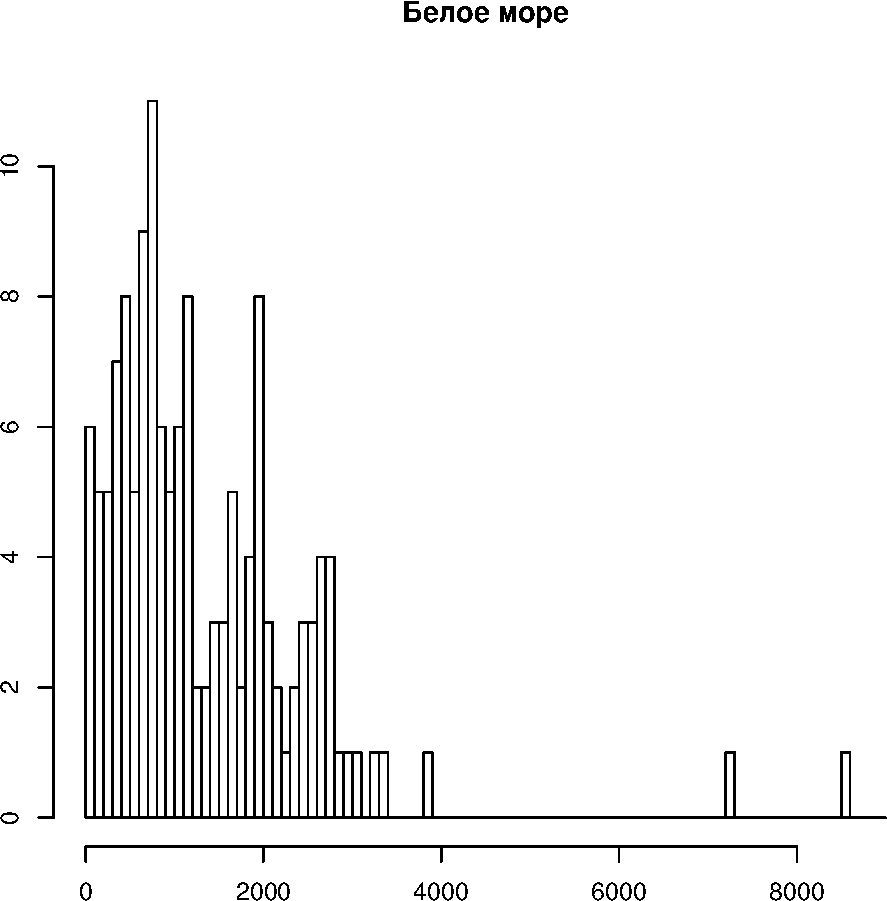
\includegraphics[height=.3\textheight]{../All_N/Nmean_hist_White.pdf}
		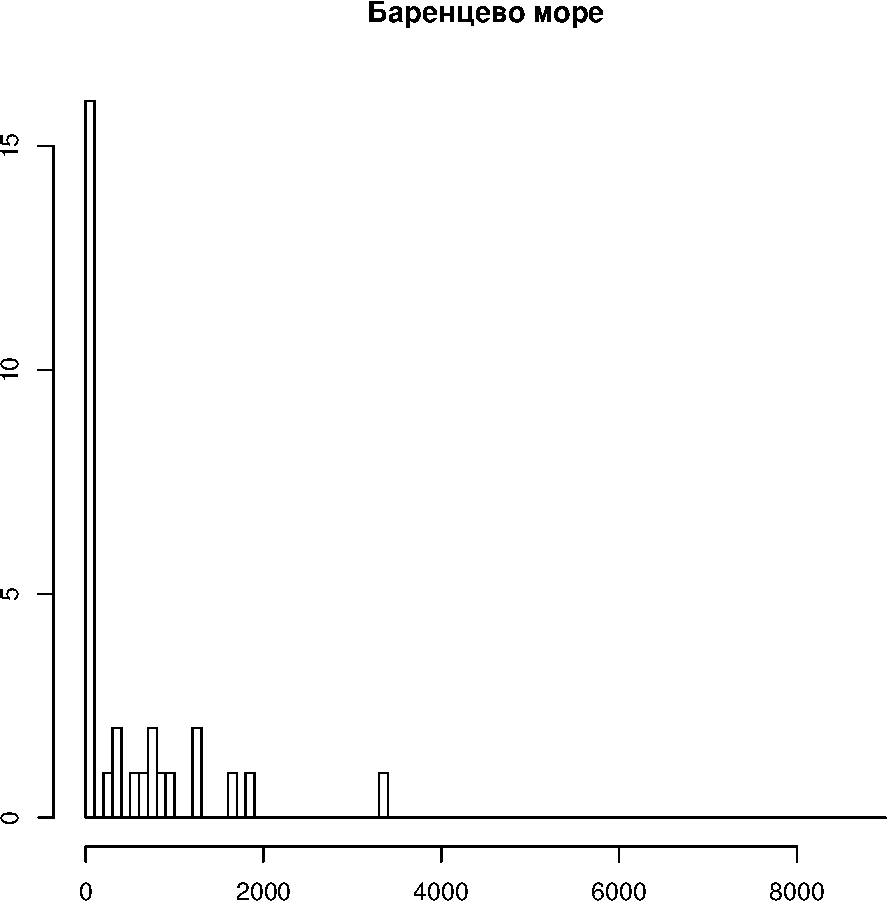
\includegraphics[height=.3\textheight]{../All_N/Nmean_hist_Barents.pdf}
	\caption{Частота встречаемости поселений с различным обилием {\it Macoma balthica}}
	{\footnotesize Примечание: по оси $X$ --- средняя численность {\it Macoma balthica}, экз./м$^2$ (шаг --- $100$~экз./м$^2$), по оси $Y$ 	--- частота встречаемости}
	\label{ris:Nmean_hist}
	\end{figure}
%
Наиболее часто встречаются поселения со средней численностью $700-800$~экз./м$^2$.
Отдельные районы Кандалакшского залива Белого моря не отличались по средней численности маком ($Kruskal-Wallis\ \chi^2 = 5,6$, $p = 0,2$). 
При сравнении средних обилий маком на разных участках в пределах одного горизонта не показало достоверных отличий (табл.~\ref{tab:Nmean_Kruskal_mareography_White}).
%
	\begin{table}[ht]
	\caption{Сравнение среднего обилия {\it M.~balthica} в пределах одного мареографического уровня в Белом море}
	\label{tab:Nmean_Kruskal_mareography_White}
	\begin{tabular}{|*{4}{p{0.2\textwidth}|}} \hline
	ма\-ре\-ографи\-ческий уровень & $Kruskal-Wallis\ \chi^2$ & $df$ & $p$ \\
	\hline
	СГЛ & $2,7$ & $5$ & $0,7$ \\
	\hline
	НГЛ & $5,8$ & $4$ & $0,2$ \\
	\hline
	ноль глубин & $0,16$ & $1$ & $0,7$ \\
	\hline
	ВСЛ & $1$ & $1$ & $0,3$ \\
	\hline
	\end{tabular}

	{\footnotesize Примечания: градации мареографического уровня: ВГЛ --- верхний горизонт литорали, СГЛ --- средний горизонт литорали, НГЛ --- нижний горидонт литорали, ВСЛ --- верхняя сублитораль}
	\end{table}
%
    Сравнение средних численностей на разных горизонтах в пределах одного участка показало различные результаты (табл.~\ref{tab:N2_area_mareography_Kruskal_White}). 
%
	\begin{table}[ht]
	\caption{Сравнение обилия {\it M.~balthica} в поселених на разном мареографическом уровне в Белом море}
	\label{tab:N2_area_mareography_Kruskal_White}
        \begin{tabular}{|p{0.25\textwidth}|*{4}{p{0.15\textwidth}|}} \hline
    участок & $Kruskal-Wallis\ \chi^2$ & $df$ & $p$ & \\
	\hline
    Клющиха & $19,7$ & $2$ & $5,2 \times 10^{-05}$ & ***\\
    \hline
    Клющиха (только литораль) & $1,1$ & $1$ & $0,31$ & \\
    \hline
    Сухая & $0,0057$ & $1$ & $0,94$ & \\
    \hline
    Лисья & $17,5$ & $2$ & $0,00016$ & ***\\
    \hline
    Лисья (только литораль) & $11,06$ & $1$ & $0,00088$ & ***\\
    \hline
    Подпахта  & $2,3$ & $1$ & $0,13$ & \\
    \hline
    Горелый & $10,2$ & $3$ & $0,01658$ & ** \\
    \hline
    материк, Лувеньга & $2,4$ & $3$ & $0,50$ &  \\
    \hline
	\end{tabular}
    {\footnotesize Примечание: достоверность различий *** --- $p<0,001$; ** --- $p<0,05$; * --- $p<0,1$.}
	\end{table}
%
Для участков в Сухой салме, проливе Подпахта, материковой литорали в Лувеньге варьирование численности между пробами перекрывало варьирование между горизонтами литорали.
При этом для участков в бухтах Клющиха и Лисья и на о.~Горелом Лувеньгских шхер  было показано достоверное влияние мареографического уровня на обилие маком. 
Интересно отметить, что в бухте Клющиха численность маком на нижнем и среднем горизонтах литорали не отличается ($403$~($7$)~экз./м$^2$), но в сублиторали она значительно выше ($1136$~($5$)~экз./м$^2$).
В бухте Лисья ситуация отличается, обилие маком на нижнем горизонте достоверно выше ($2832$~($10$)~экз./м$^2$), чем в среднем и в сублиторали ($1346$~($16$) и $1006$~($16$)~экз./м$^2$, соответсвенно). 



	\subsection{Баренцево море}

В Баренцевом море данные по обилию маком были получены для $12$ участков Мурманского побережья.
Минимальная средняя численность составляла $30$~экз./м$^2$ (г.~Дальнезеленецкая), что сравнимо с показателями для Белого моря. 
Максимальная средняя численность была значительно меньше, чем беломорская --- $3350$~экз./м$^2$ (Абрам-мыс) (табл.~\ref{tab:mean_N_Barents}). 
	\begin{footnotesize}
	\begin{longtable}{|p{2cm}|p{3cm}|p{1cm}|p{2cm}|p{1.5cm}|p{1cm}|*{3}{c|}}
	\caption{Средняя численность {\it Macoma balthica} на различных участках Баренцева моря}\label{tab:mean_N_Barents}\\
	\hline
	Район & Участок & год & ма\-ре\-ографи\-ческий уровень & число повторностей & площадь учета & $N$, экз./м$^2$ & $S_x$  & $D, \%$ 
	\\ \hline \endfirsthead
	\hline
	\multicolumn{9}{|c|}{продолжение таблицы \ref{tab:mean_N_Barents}} \\ \hline
	Район & Участок & год & ма\-ре\-ографи\-ческий уровень & число повторностей & площадь учета & $N$, экз./м$^2$ & $S_x$  & $D, \%$ 
	\\ \hline \endhead
	\hline 
	\multicolumn{9}{|c|}{продолжение таблицы \ref{tab:mean_N_Barents} на следующей странице}
	\\ \hline \endfoot
	\endlastfoot
	Западный Мурман & Ура-губа & 2005 & СГЛ & 3 & 1/30 & 1267 & 288,8 & 23
		\\ \cline{2-9}
		 & Печенга & 2005 & СГЛ & 3 & 1/30 & 767 & 218,6 & 29
		\\ \hline
	Кольский Залив & Северное Нагорное & 2005 & СГЛ & 2 & 1/30 & 390 & 90,0 & 23
		\\ \cline{2-9}
		 & Абрам-мыс & 2005 & СГЛ & 2 & 1/30 & 3350 & 520,0 & 16
		\\ \cline{3-9}
		 &  & 2008 & СГЛ & 5 & 1/20 & 540 & 208,5 & 39
		\\ \cline{4-9}
		 &  &  & НГЛ & 5 & 1/20 & 1804 & 78,6 & 4
		\\ \cline{2-9}
		 & Ретинское & 2005 & СГЛ & 2 & 1/30 & 660 & 300,0 & 45
		\\ \cline{2-9}
		 & Пала-губа & 2007 & СГЛ & 16 & 1/30 & 936 & 76,4 & 8
		\\ \cline{3-9}
		 &  & 2007 осень & НГЛ & 36 & 1/30 & 790 & 61,7 & 8
		\\ \cline{3-9}
		 &  & 2008 зима & НГЛ & 11 & 1/20 & 864 & 154,4 & 18
		\\ \cline{3-9}
		 &  & 2008 & НГЛ & 10 & 1/30 & 1644 & 192,5 & 12
		\\ \hline
	Восточный Мурман & Гаврилово & 2008 & СГЛ & 5 & 1/30 & 138 & 20,3 & 15
		\\ \cline{4-9}
		 &  & 2008 & НГЛ & 5 & 1/30 & 24 & 11,2 & 47
		\\ \cline{2-9}
		 & Ярнышная & 2007 & СГЛ & 36 & 1/30 & 70 & 9,6 & 14
		\\ \cline{3-9}
		 &  & 2008 & ВГЛ & 5 & 1/30 & 414 & 47,8 & 12
		\\ \cline{4-9}
		 &  & & НГЛ & 5 & 1/30 & 387 & 109,1 & 28
		\\ \cline{2-9}
		 & Дальнезеленецкая & 2002 & СГЛ & 43 & 1/30 & 52 & 7,0 & 13
		\\ \cline{3-9}
		 &  & 2003 & СГЛ & 48 & 1/30 & 34 & 6,6 & 20
		\\ \cline{3-9}
		 &  & 2004 & СГЛ & 44 & 1/30 & 32 & 5,3 & 16
		\\ \cline{3-9}
		 &  & 2005 & СГЛ & 30 & 1/30 & 30 & 4,5 & 15
		\\ \cline{3-9}
		 &  & 2006 & СГЛ & 28 & 1/30 & 39 & 6,0 & 16
		\\ \cline{3-9}
		 &  & 2007 & СГЛ & 33 & 1/30 & 72 & 6,6 & 9
		\\ \cline{3-9}
		 &  & 2008 & СГЛ & 72 & 1/30 & 72 & 5,5 & 8
		\\ \cline{4-9}
		 &  &  & ВГЛ & 10 & 1/30 & 30 & 8,9 & 30
		\\ \cline{4-9}
		 &  &  & НГЛ & 5 & 1/30 & 42 & 7,3 & 17
		\\ \cline{2-9}
		 & Шельпино & 2008 & СГЛ & 5 & 1/30 & 54 & 11,2 & 21
		\\ \cline{4-9}
		 &  &  & ВГЛ & 5 & 1/30 & 36 & 17,5 & 49
		\\ \cline{2-9}
		 & Порчниха & 2007 & СГЛ & 32 & 1/30 & 87 & 10,8 & 12
		\\ \cline{3-9}
		 &  & 2008 & СГЛ & 5 & 1/30 & 60 & 13,4 & 22
		\\ \cline{2-9}
		 & Ивановская & 2008 & ВСЛ & 5 & 1/20 & 1208 & 72,8 & 6
		\\ \hline
	\multicolumn{9}{p{16cm}}{Примечания: градации мареографического уровня: ВГЛ --- верхний горизонт литорали, СГЛ --- средний 	горизонт литорали, НГЛ --- нижний горидонт литорали, ВСЛ --- верхняя сублитораль. 

	$N$, экз./м$^2$ --- средняя численность {\it M.~balthica}. 
	$S_x$ --- ошибка среднего.
	 $D, \%$ ---  точность учета.
	
	В обозначении числа повторностей индекс ''и'' означает интегральную пробу, в этом случае в графе площадь учета указано сколько проб какой площади 	объединялись в одну.}
	\end{longtable}
	\end{footnotesize}
%
Среди иследованных, наиболее часто встречались поселения со средним обилием менее $100$~экз./м$^2$ (рис.~\ref{ris:N_region_Barents}).

Важно отметить, что для Мурманского побережья Баренцева моря показаны различия между отдельными районами: Западным, Восточным Мурманом и Кольским заливом (\ref{} \textcolor{red}{Гурьянова и ко?}). 
Это подтверждается нашими данными (рис.~\ref{ris:N_region_Barents}) по размаху варьирования среднего обилия в пределах районов ($Kruskal-Wallis\ \chi^2 = 17,6$, $p = 0,00015$).
%
	\begin{figure}[h]
		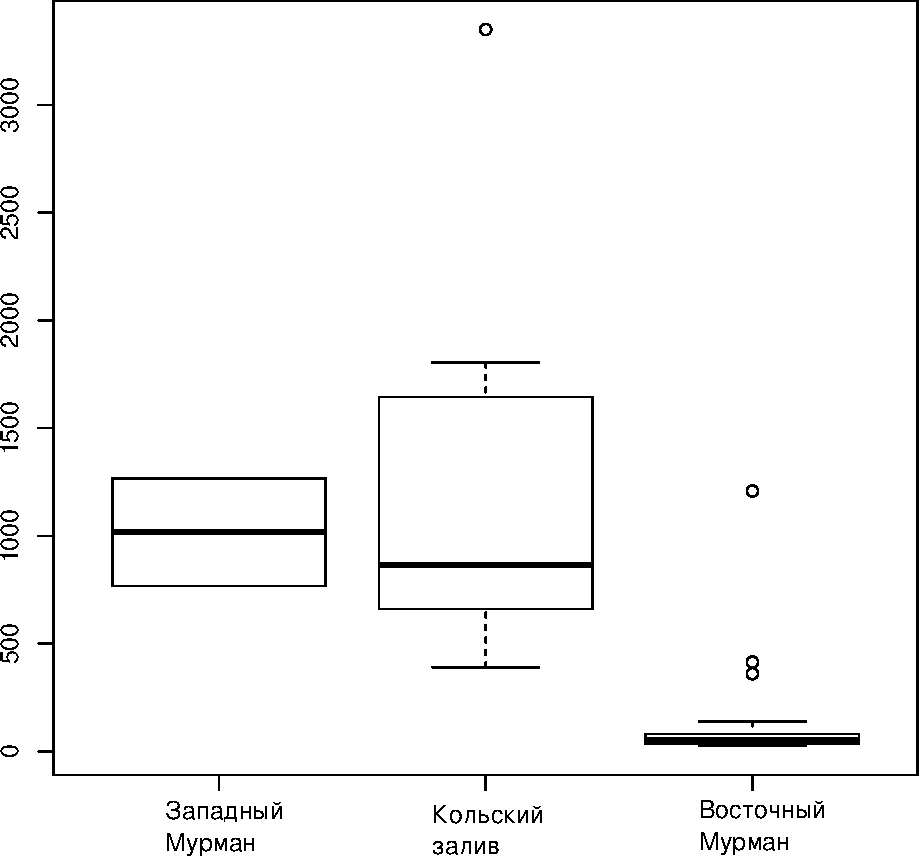
\includegraphics{../All_N/Nmean_region_Barents1.pdf}
	\caption{Варьирование среднего обилия {\it Macoma balthica} в разных районах Мурманского побережья Баренцева моря}
	{\footnotesize Примечание: По оси абсцисс --- численность {\it M.~balthica}, ~экз./м$^2$.

	На графике: жирная горизонтальная линия --- медиана, границы ''ящика'' --- 1 и 3 квартили, ''усы'' --- $1,5$ интерквартильного расстояния, точки - значения выпадающие за $1,5$ интерквартильных расстояния}
	\label{ris:N_region_Barents}
	\end{figure}
%
На литорали Восточного Мурмана численность {\it M.~balthica} в основном не превышала $100$~экз./м$^2$. 
Единственное исключение ---\ литораль губы Ярнышная, где численность маком достигала $410$~($12$)~экз./м$^2$. 
Между тем, на единственном участке, где были учеты в сублиторали, в губе Ивановской, численность на порядок выше, чем ее значения на литорали Восточного мурмана, и составляет $1200$~экз./м$^2$. 
В Кольском заливе минимальные значения обилия были отмечены на литорали в районе Северного Нагорного ($390$~($23$)~экз./м$^2$). 
Максимальных значений численности как для региона, так и для всей исследованной части Мурманского побережья, достигали поселения маком на учатске в районе Абрам-мысса ($3350$~($16$)~экз./м$^2$). 
На Западном Мурмане обилие флуктуировало вокруг $1000$~экз./м$^2$.  

При сравнении численности маком на различных мареографических уровнях различия между горизонтами литорали были показаны для губ Гаврилово и Ярнышная (табл.~\ref{tab:N2_area_mareography_Kruskal_Barents}).
В Гаврилово средняя численность {\it M.~balthica} в среднем горизонте литорали превышала аналогичные значения для нижнего горизонта на порядок ($138$~($15$) и $24$~($47$)~экз./м$^2$, соответственно).
В губе Ярнышная численность маком в верхнем и нижнем горизонтах не различалась ($414$~($12$) и $360$~($43$)~экз./м$^2$, соответсвенно), в то время как в среднем горизонте литорали она была значительно ниже ($70$~($14$)~экз./м$^2$).  
%
	\begin{table}[ht]
	\caption{Сравнение обилия {\it Macoma balthica} в поселених на разном мареографическом уровне в Баренцевом море}
	\label{tab:N2_area_mareography_Kruskal_Barents}
        \begin{tabular}{|p{0.25\textwidth}|*{4}{p{0.15\textwidth}|}} \hline
    участок & $Kruskal-Wallis\ \chi^2$ & $df$ & $p$ & \\
    \hline
    Абрам-мыс &  $1,5$ & $1$ & $0,224$ & \\
    \hline
    Пала-губа & $0,4$ & $1$ & $0,54$ & \\
    \hline
    Гаврилово & $6,9$ & $1$ & $0,0084$ & *** \\
    \hline
    Ярнышная & $19,4$ &  $2$ &  $6,09 \times 10^{-5}$ & *** \\
    \hline
    Дальнезеленецкая & $1,6$ & $2$ & $0,45$ & \\
    \hline
    Шельпино & $0,7$ & $1$ & $0,39$ & \\
    \hline
	\end{tabular}
    {\footnotesize Примечание: достоверность различий *** --- $p<0,001$; ** --- $p<0,05$; * --- $p<0,1$.}
	\end{table}
%

    \subsection{Влияние состава грунта на численность {\it Macoma balthica}}
Нет сомнений, что основной параметр, определяющий обилие маком ---\ это доступные пищевые   ресурсы.   
Косвенным   показателем   наличия   пищевых   ресурсов   служит гранулометрический состав грунта и общее содержание органических веществ. 
Поэтому по полученым для участков на Баренцевом море данным мы провели корреляционный анализ связи среднего обилия маком на участке с характеристиками  грунта.  
В   результате  оказалось,   что   соотношение   песчаных  фракций   различного   размера влияет   на   обилие  {\it M.~balthica}  (табл.~\ref{tab:grunt_N_correlation_Barents}).  
%
	\begin{table}[ht]
	\caption{Сравнение обилия {\it Macoma balthica} в поселених на разном мареографическом уровне в Баренцевом море}
    \label{tab:grunt_N_correlation_Barents}
     \begin{tabular}{|*{4}{p{0.15\textwidth}|}} \hline
    фракция & $R_s$ & $p-value$ & \\
    \hline
    $>10$~мм & $-0,2$ &  $0,36$ & \\
    \hline
    $10 - 5$~мм & $-0,01$ & $0,98$ & \\
    \hline
    $5 - 3$~мм & $0,07$ & $0,87$ & \\
    \hline
    $3 - 1$~мм & $0,12$ & $0,78$ & \\
    \hline
    $1 - 0,5$~мм & $-0,74$ & $0,04$ & ** \\
    \hline
    $0,5 - 0,25$~мм & $-0,67$  & $0,07$ & * \\
    \hline
    $0,25 - 0,1$~мм & $0,71$ & $0,04$ & ** \\
    \hline
    $<0,1$~мм & $0,6$ &  $0,12$ & \\
    \hline
    доля органических веществ & $0,36$ & $0,38$ & \\
    \hline
	\end{tabular}
    
    {\footnotesize Примечание: $R_s$ --- корреляция Спирмена. \\
    достоверность различий *** --- $p<0,001$; ** --- $p<0,05$; * --- $p<0,1$.}
	\end{table}
%
При   этом  наблюдается   достоверная   отрицательная корреляция численности маком с долей крупного  песка и положительная — с долей мелкого.


%% для компиляции в lualatex!!
\documentclass[12pt, a4paper]{article}
\usepackage[english,russian]{babel}
\usepackage[warn]{mathtext}
%\usepackage[T2A]{fontenc}
%\usepackage[utf8]{inputenc}

\usepackage{xecyr} % Продукт Вашего покорного слуги ;)

\setmainfont{DejaVu Serif}

\usepackage{color}
\usepackage{amssymb,amsmath}
\usepackage{graphicx}
\usepackage{multicol}

\textheight=24cm           % высота текста
\textwidth=16cm            % ширина текста
\oddsidemargin=0pt         % отступ от левого края
\topmargin=-1.5cm          % отступ от верхнего края
\parindent=24pt            % абзацный отступ
\parskip=0pt               % интервал между абзацами
\tolerance=2000            % терпимость к "жидким" строкам
\flushbottom               % выравнивание высоты страниц
%\def\baselinestretch{1.5} % печать с большим интервалом

%\title{}
%\author{\copyright~~С.А.~Назарова \thanks{e-mail:~sophia.nazarova@gmail.com}}
%\date{}

\begin{document}



%\maketitle

%Эстуарий Лувеньги
\begin{figure}[h]

\begin{multicols}{3}
\hfill
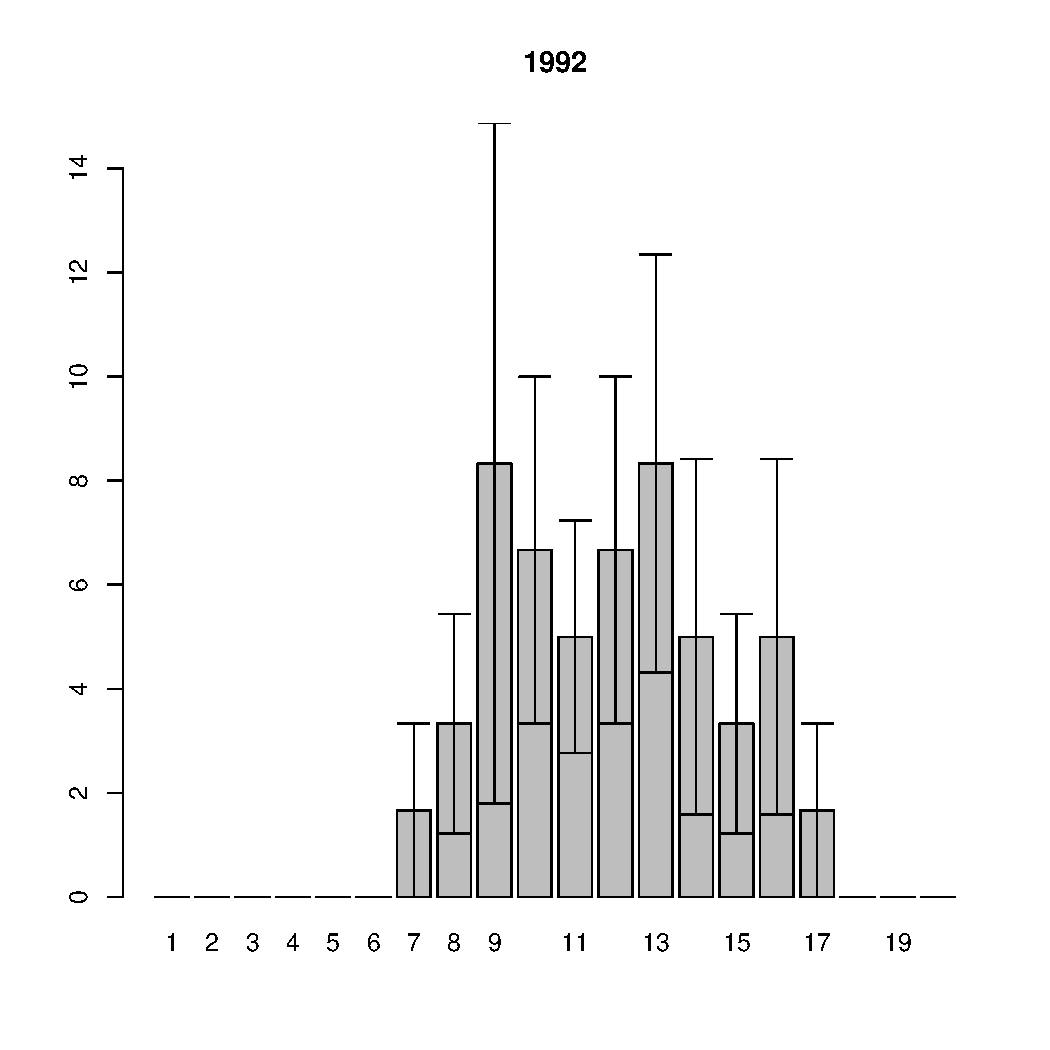
\includegraphics[width=60mm]{../White_Sea/Estuatiy_Luvenga/sizestr_1992_.pdf}
\hfill
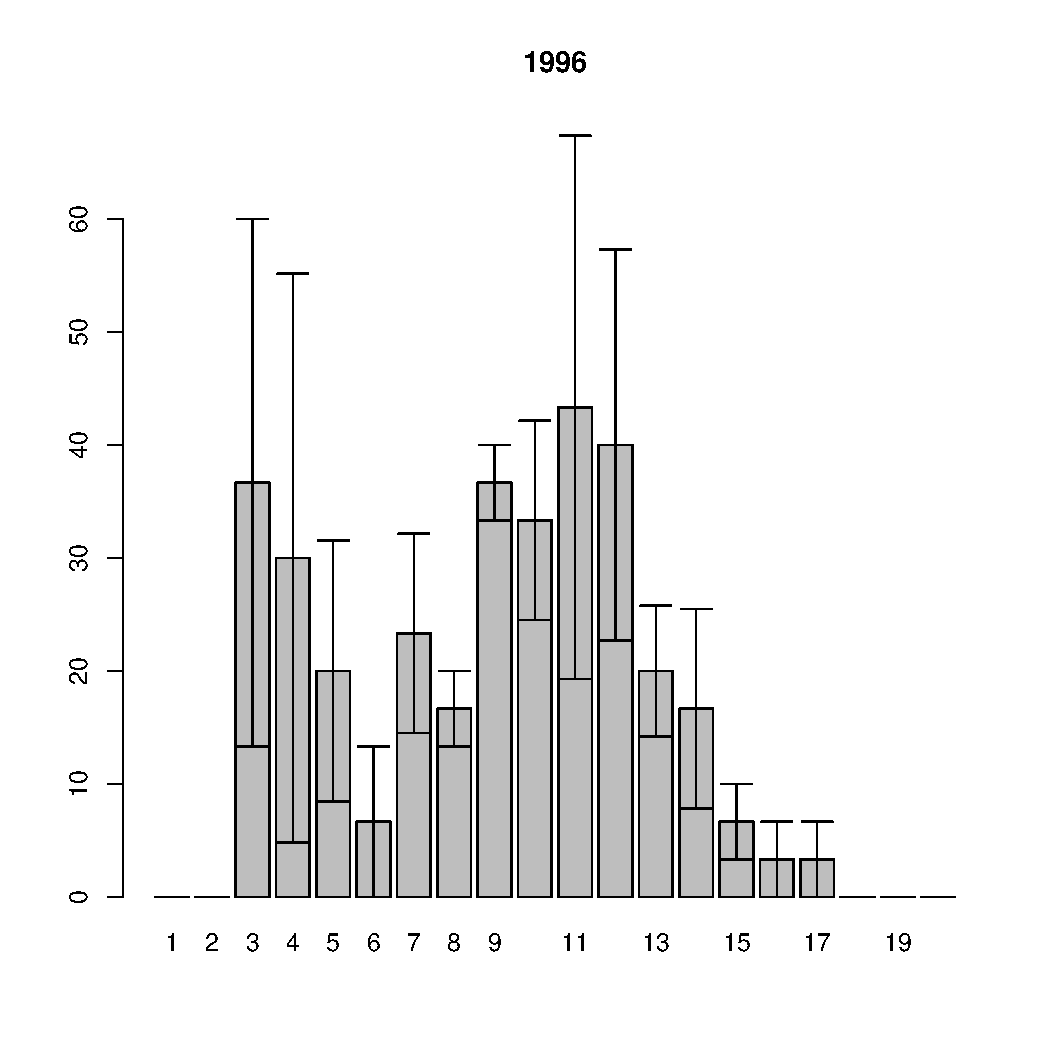
\includegraphics[width=60mm]{../White_Sea/Estuatiy_Luvenga/sizestr_1996_.pdf}
\hfill
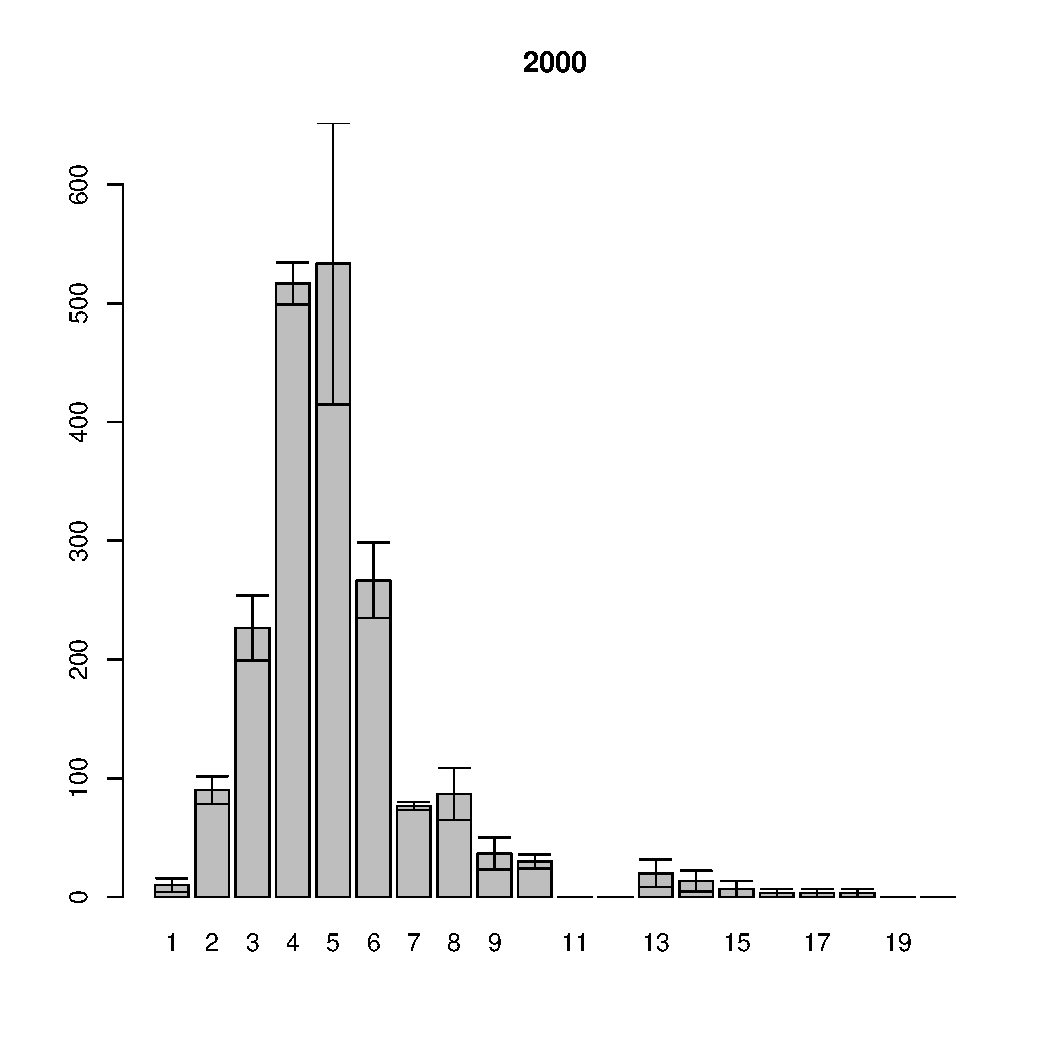
\includegraphics[width=60mm]{../White_Sea/Estuatiy_Luvenga/sizestr_2000_.pdf}
\end{multicols}

%\smallskip


\begin{multicols}{3}
\hfill
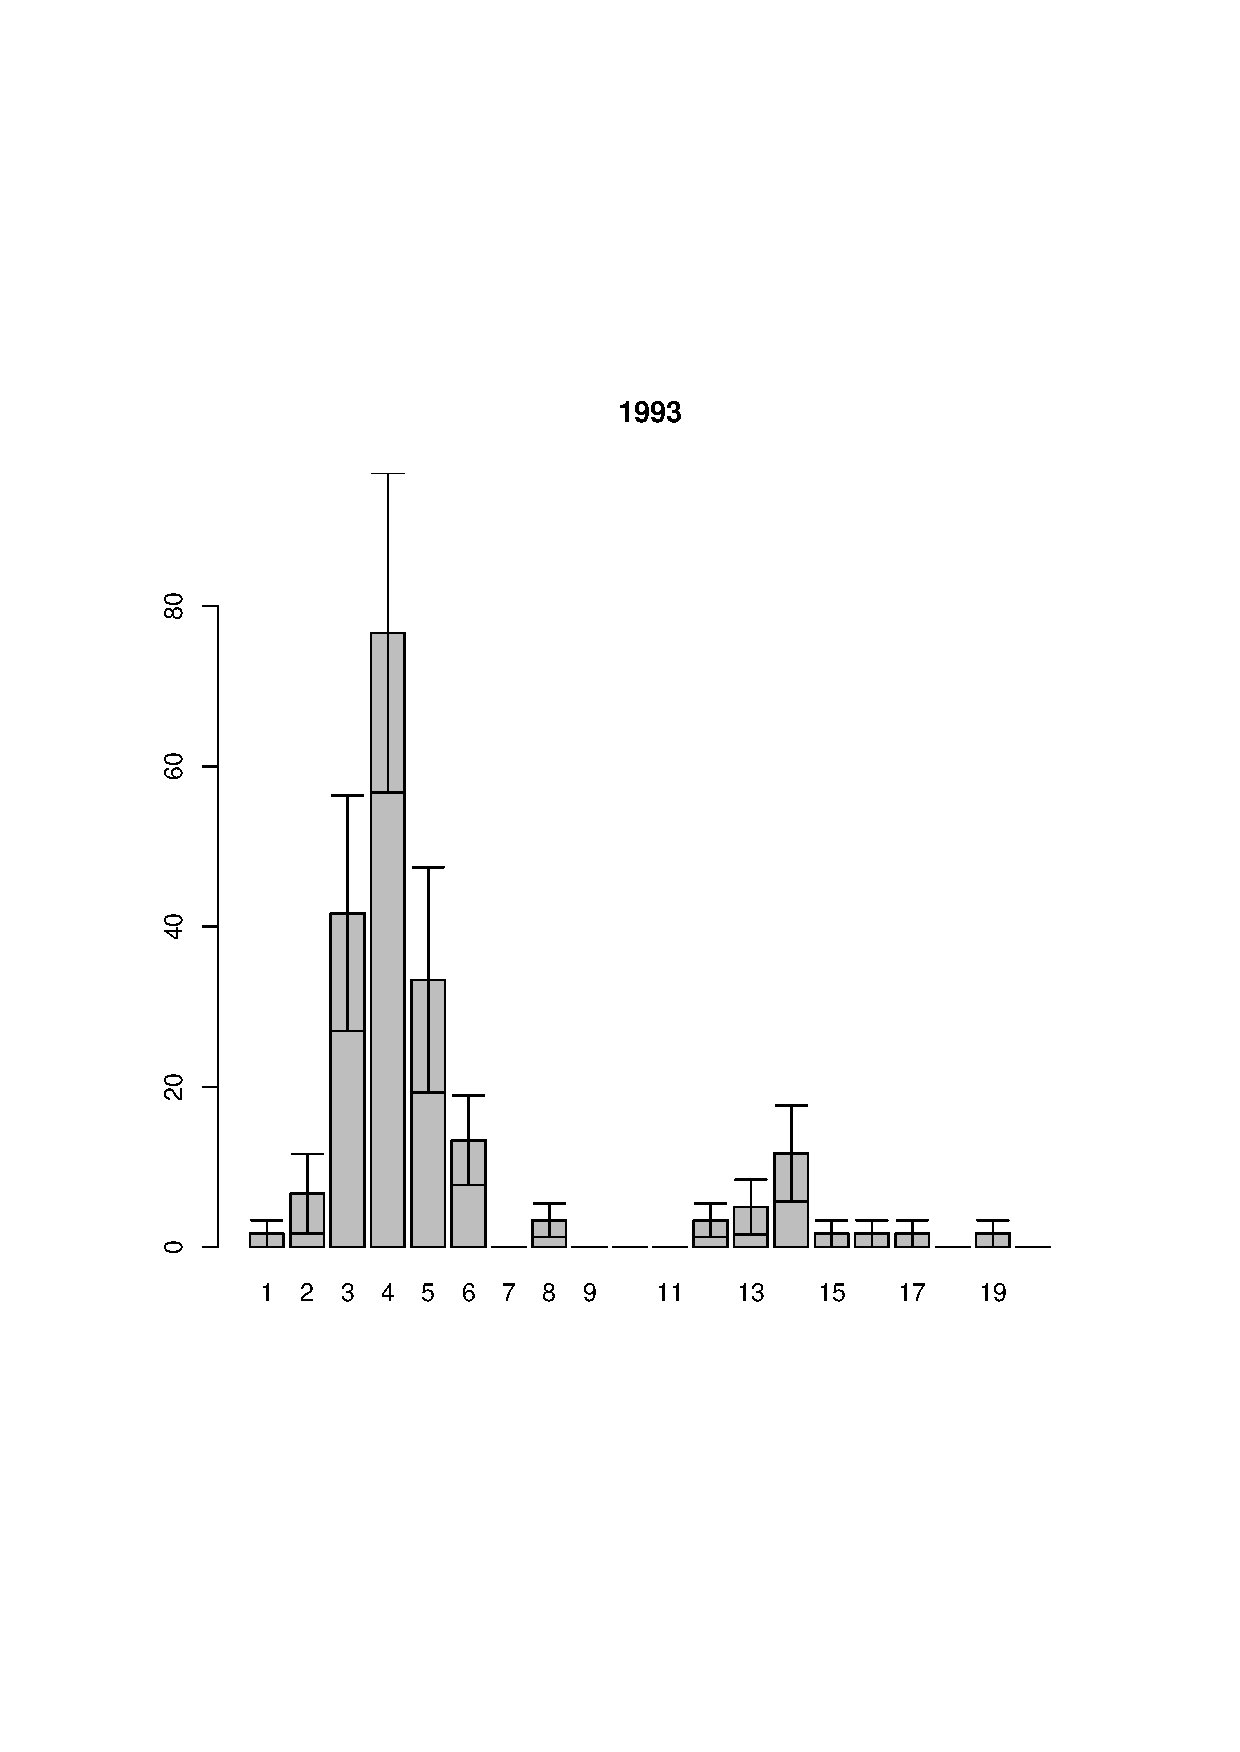
\includegraphics[width=60mm]{../White_Sea/Estuatiy_Luvenga/sizestr_1993_.pdf}
\hfill
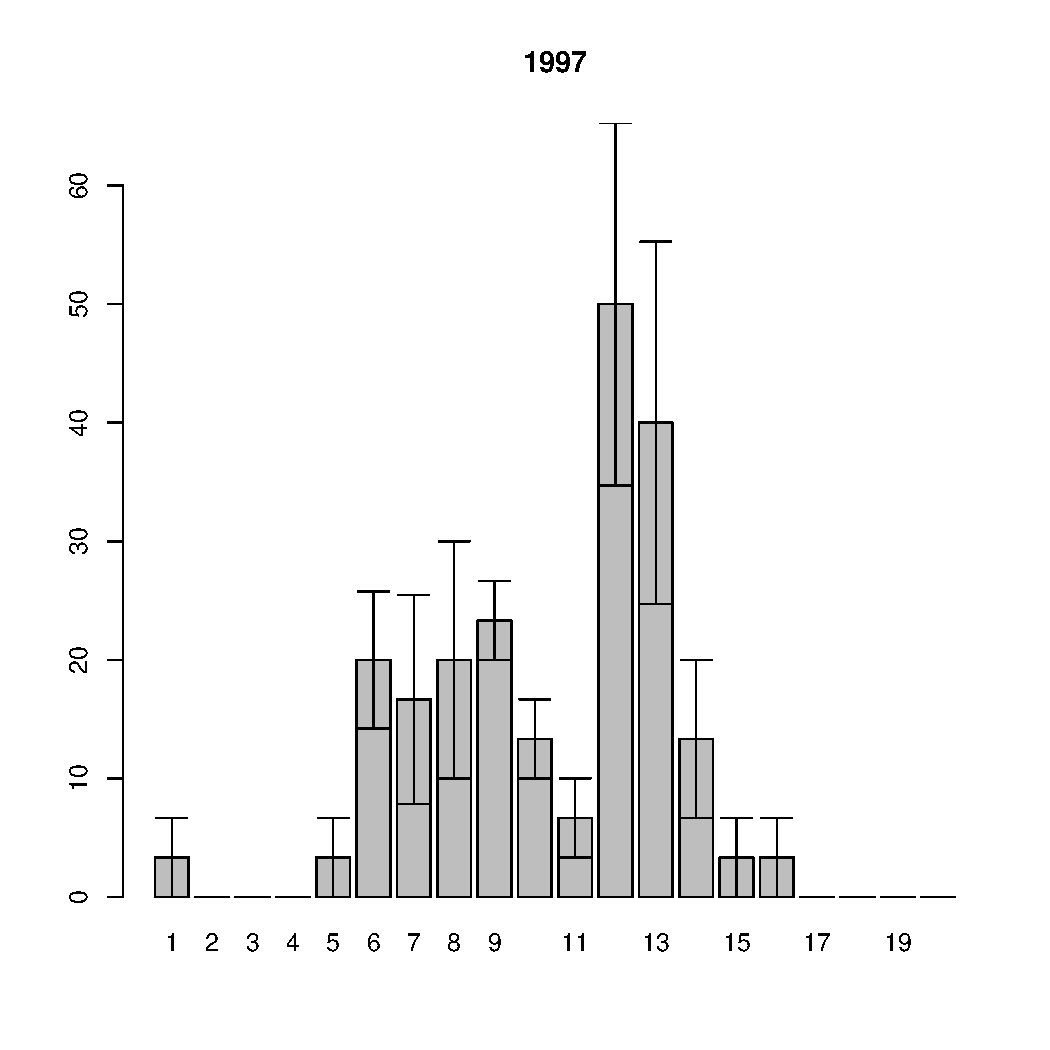
\includegraphics[width=60mm]{../White_Sea/Estuatiy_Luvenga/sizestr_1997_.pdf}
\hfill
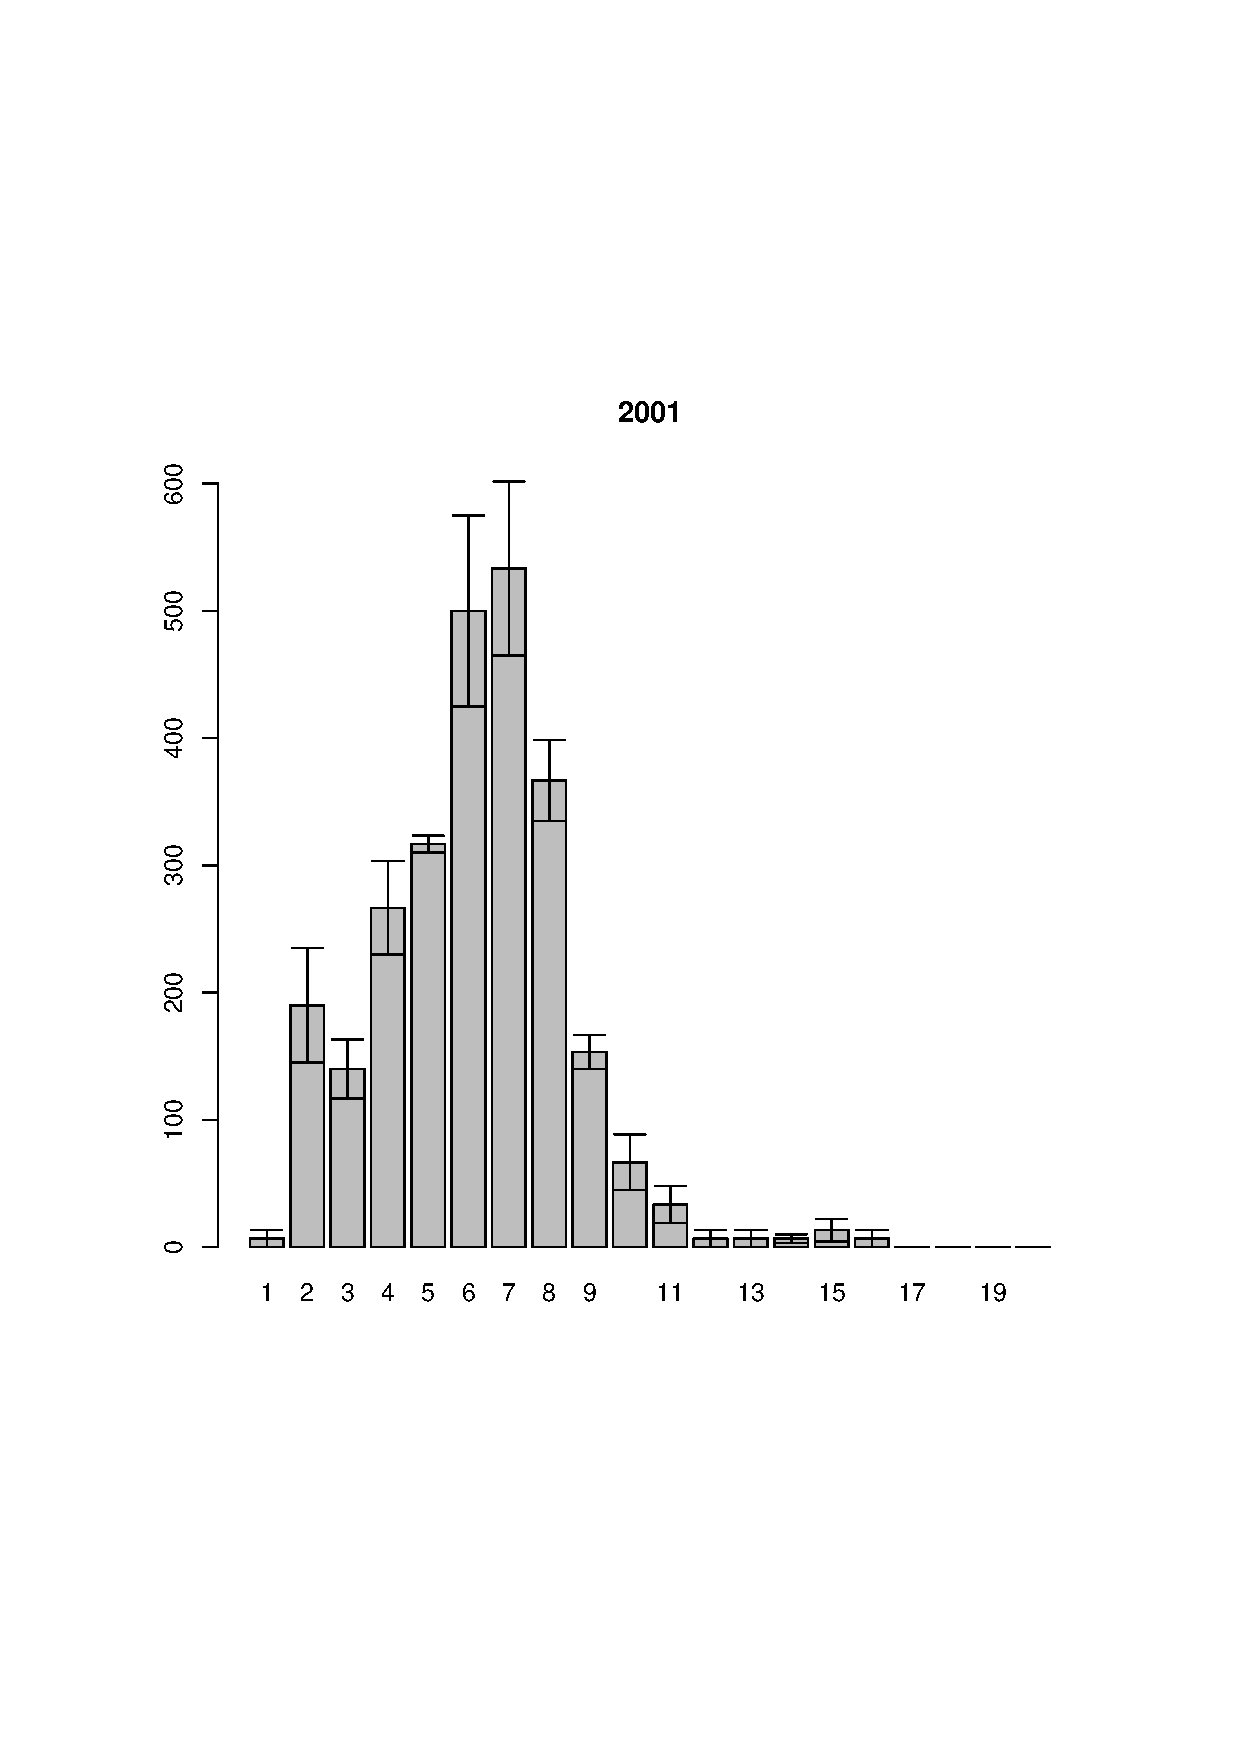
\includegraphics[width=60mm]{../White_Sea/Estuatiy_Luvenga/sizestr_2001_.pdf}
\end{multicols}

%\smallskip

\begin{multicols}{3}
\hfill
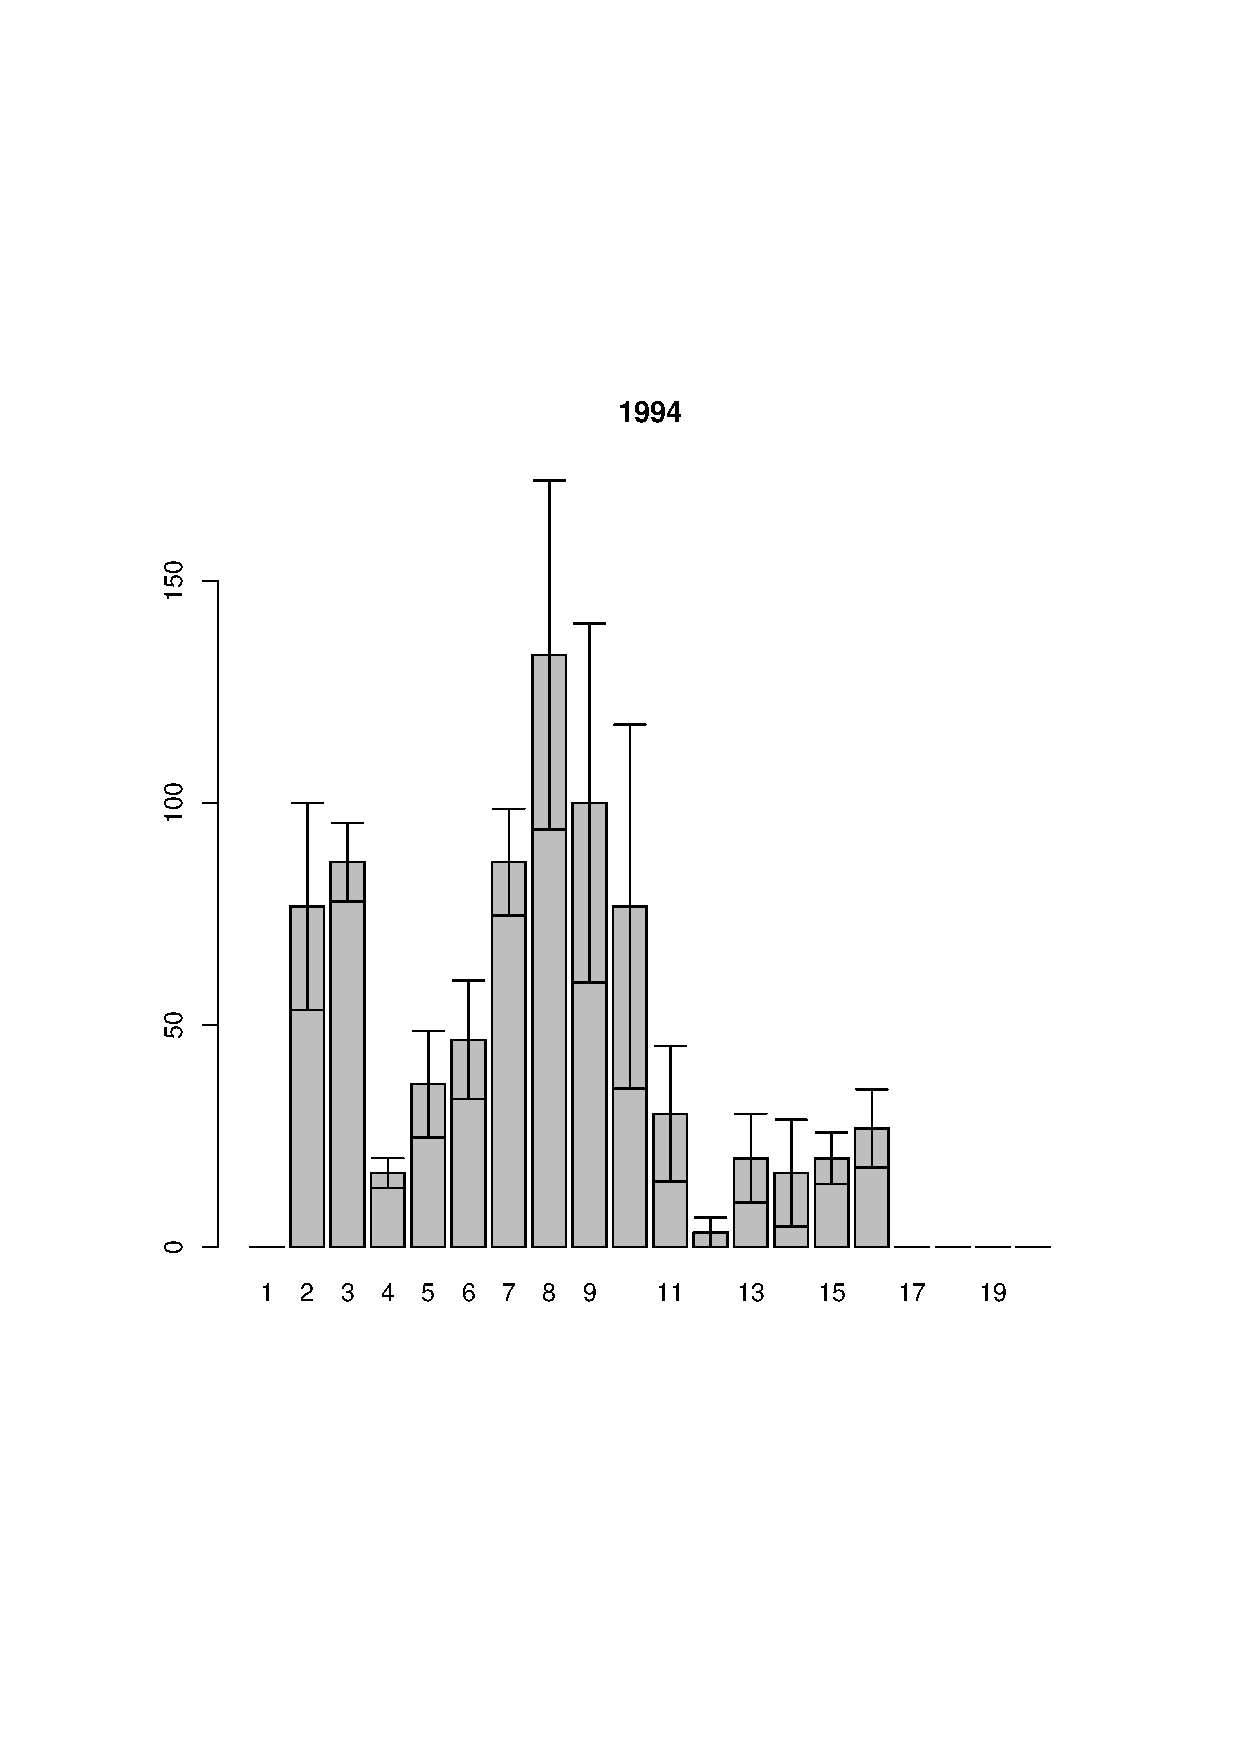
\includegraphics[width=60mm]{../White_Sea/Estuatiy_Luvenga/sizestr_1994_.pdf}
\hfill
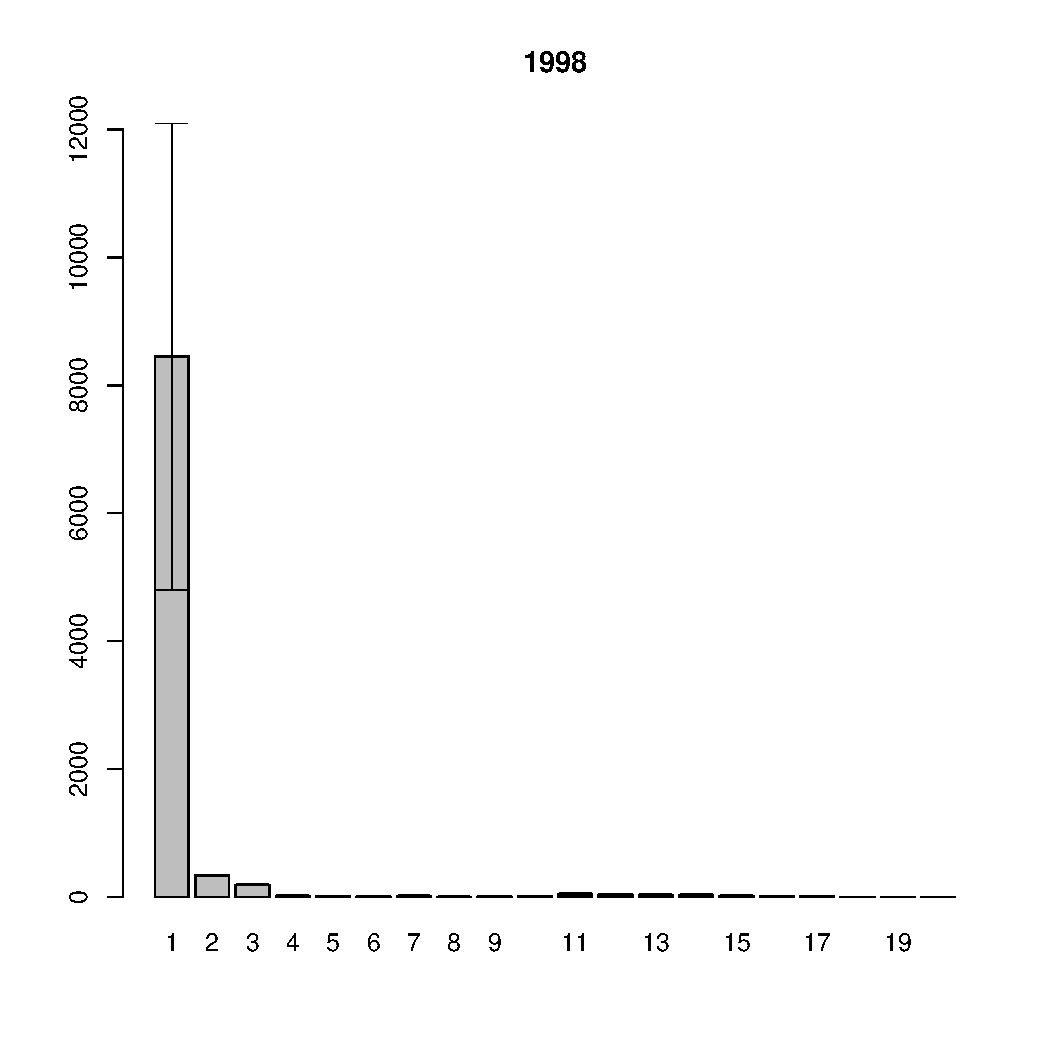
\includegraphics[width=60mm]{../White_Sea/Estuatiy_Luvenga/sizestr_1998_.pdf}
\hfill
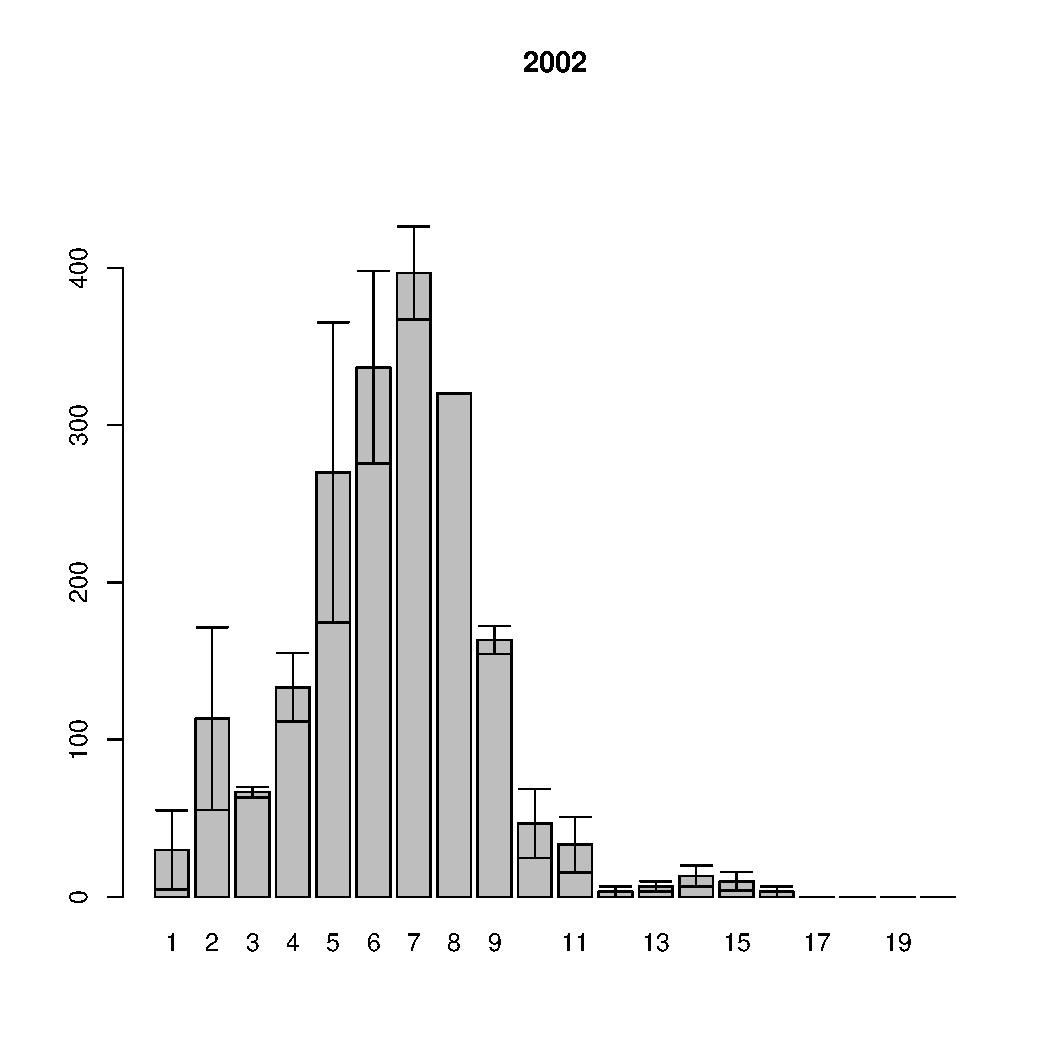
\includegraphics[width=60mm]{../White_Sea/Estuatiy_Luvenga/sizestr_2002_.pdf}
\end{multicols}

%\smallskip

\begin{multicols}{3}
\hfill
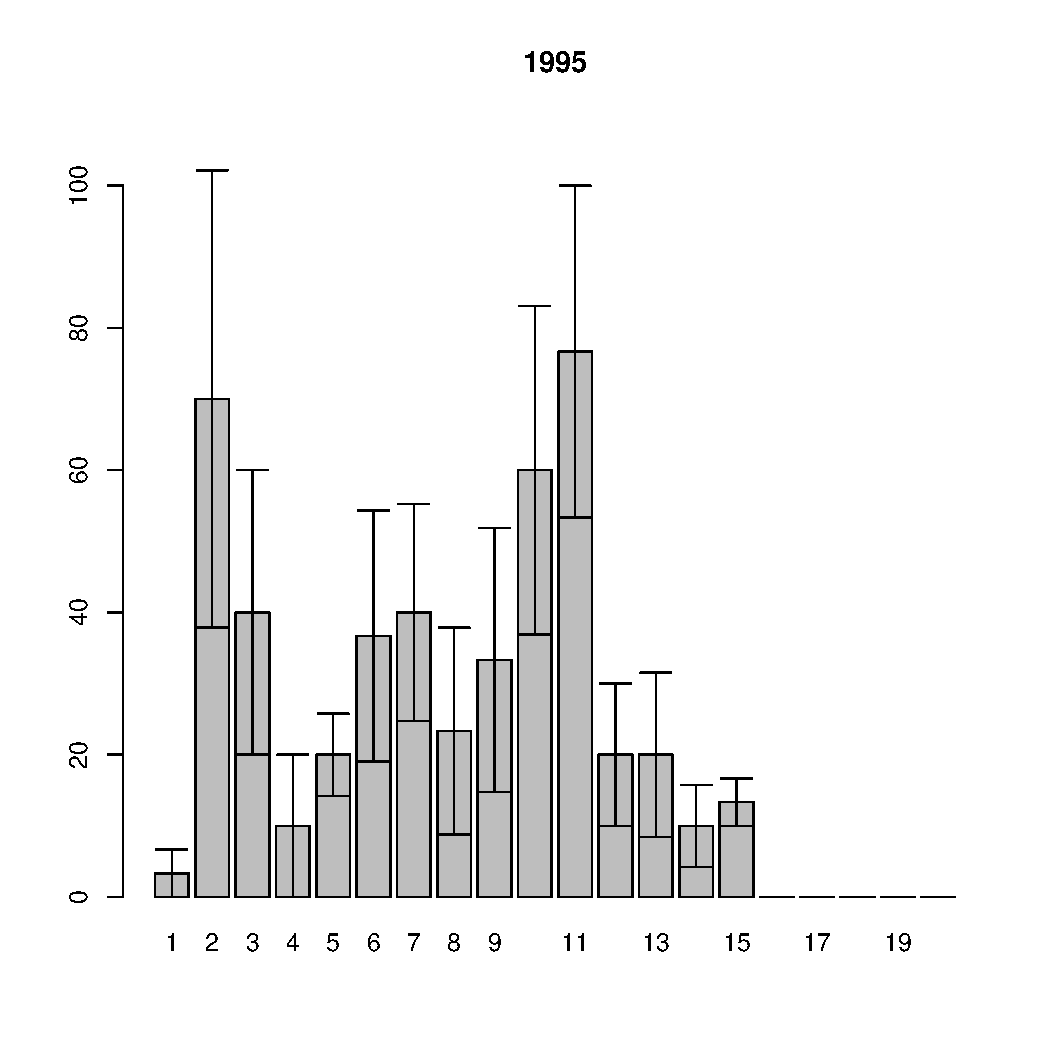
\includegraphics[width=60mm]{../White_Sea/Estuatiy_Luvenga/sizestr_1995_.pdf}
\hfill
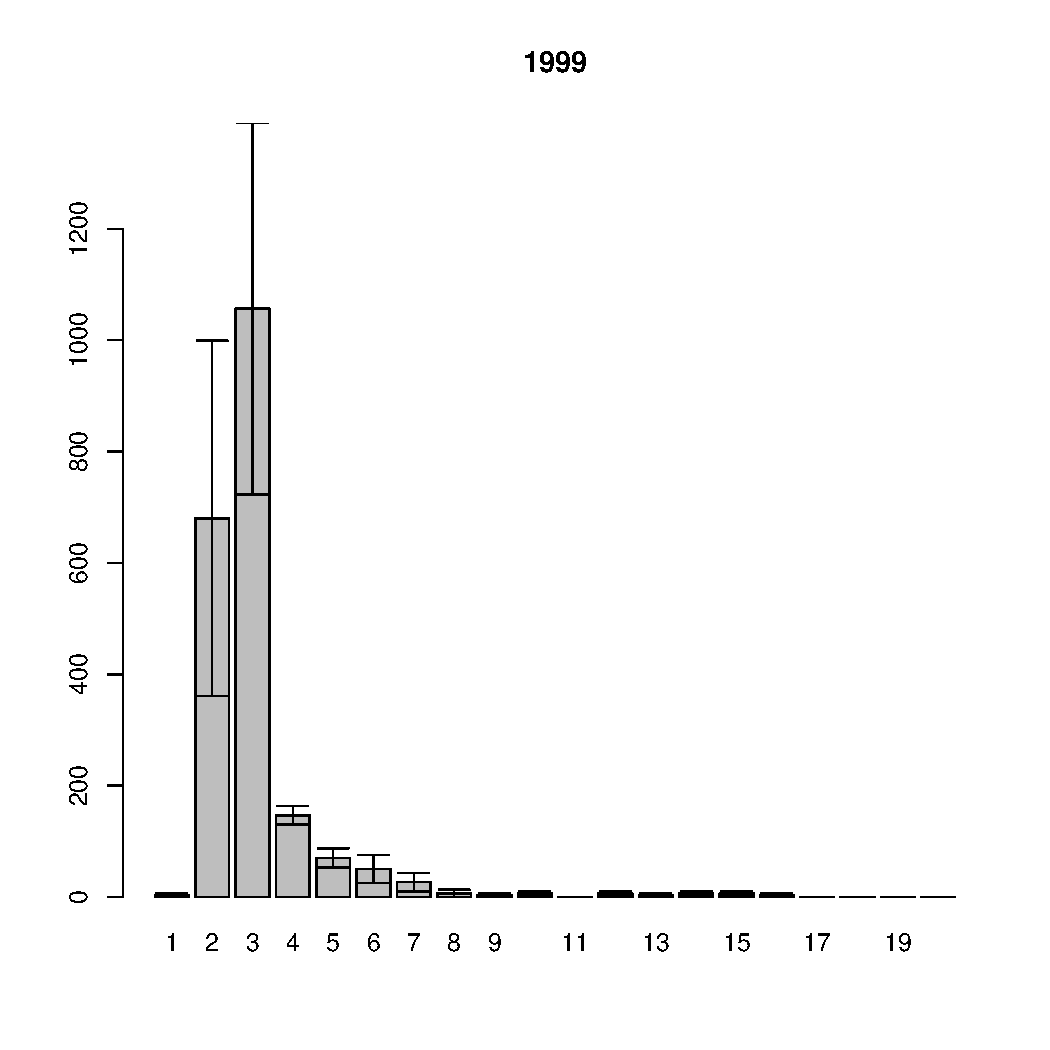
\includegraphics[width=60mm]{../White_Sea/Estuatiy_Luvenga/sizestr_1999_.pdf}
\hfill
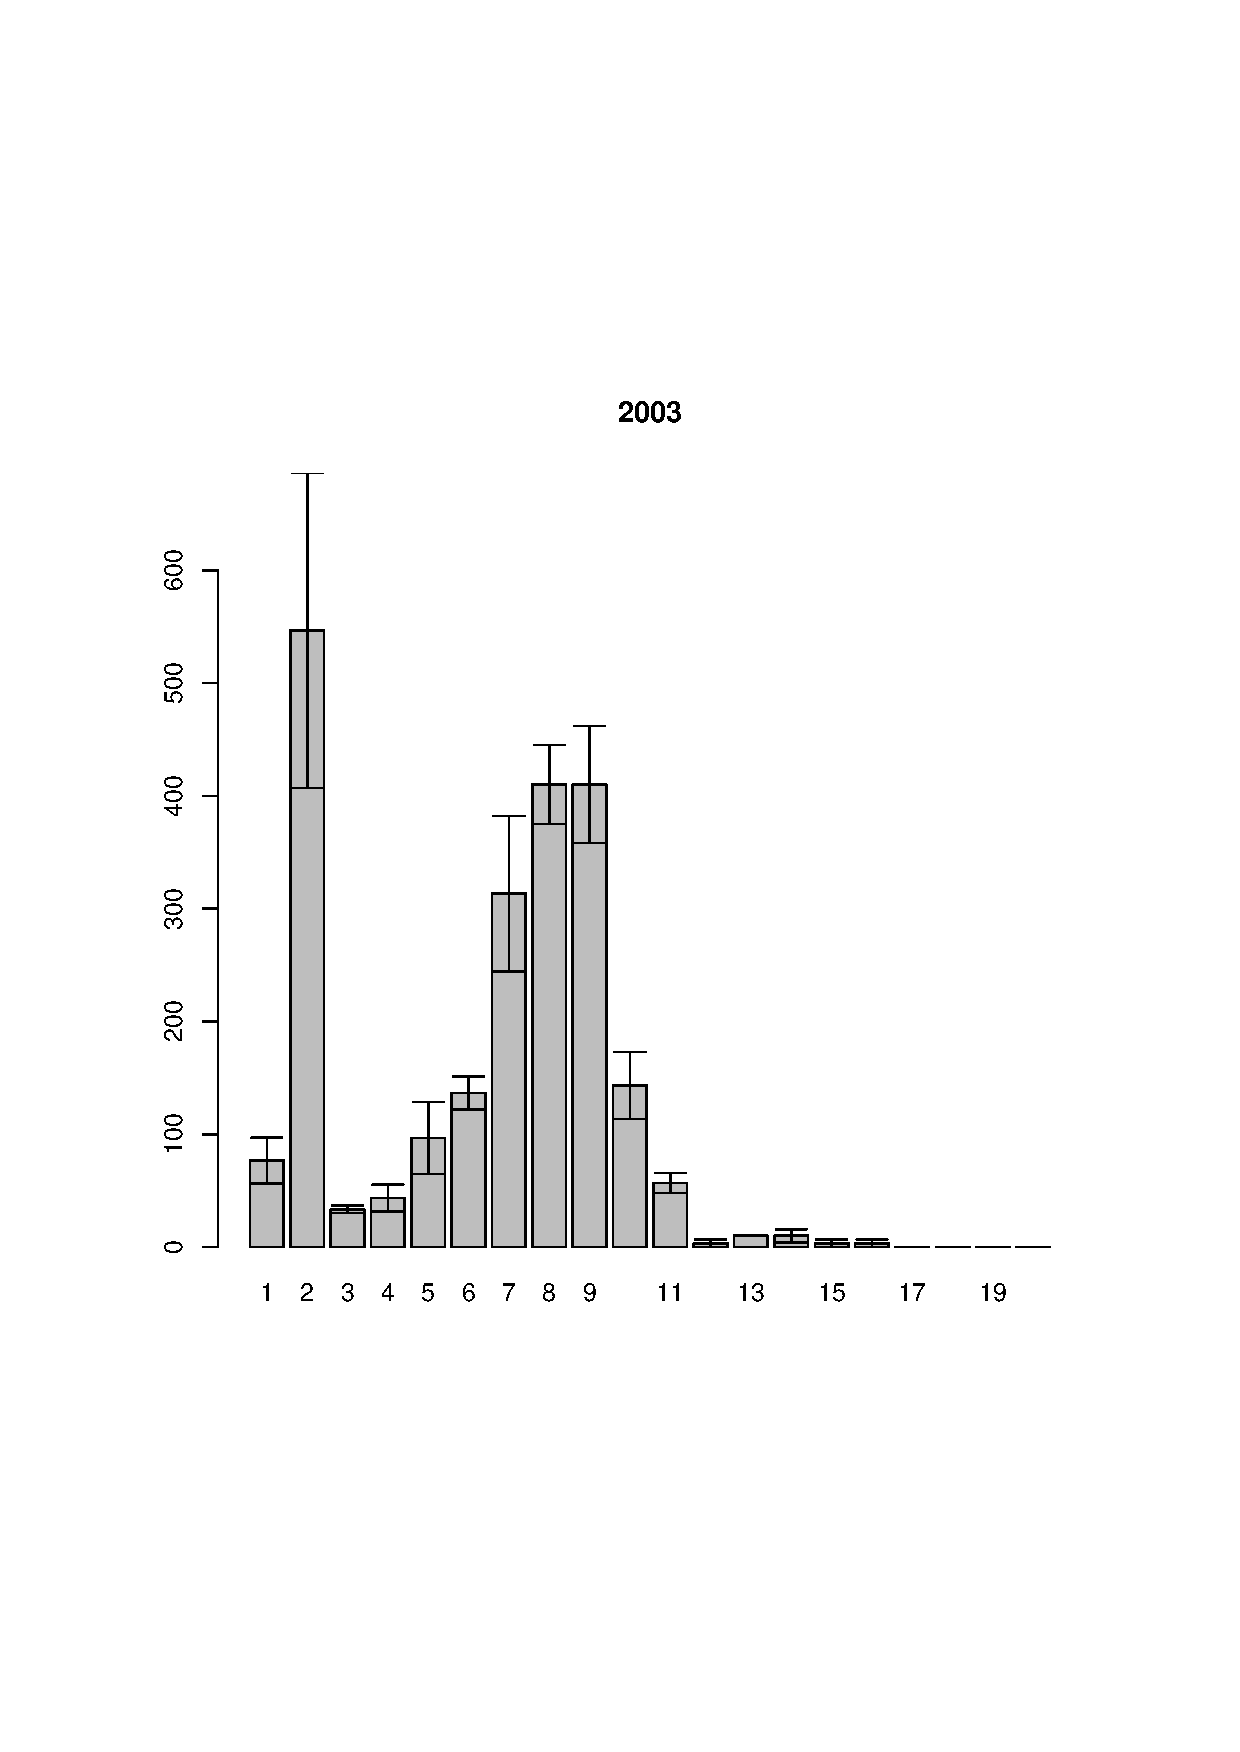
\includegraphics[width=60mm]{../White_Sea/Estuatiy_Luvenga/sizestr_2003_.pdf}
\end{multicols}


\caption{Размерная структура {\it Macoma balthica} в СГЛ эстуария р. Лувеньги}
\label{ris:size_str_estuary_Luv}
\end{figure}


\begin{figure}[h]

\begin{multicols}{3}
\hfill
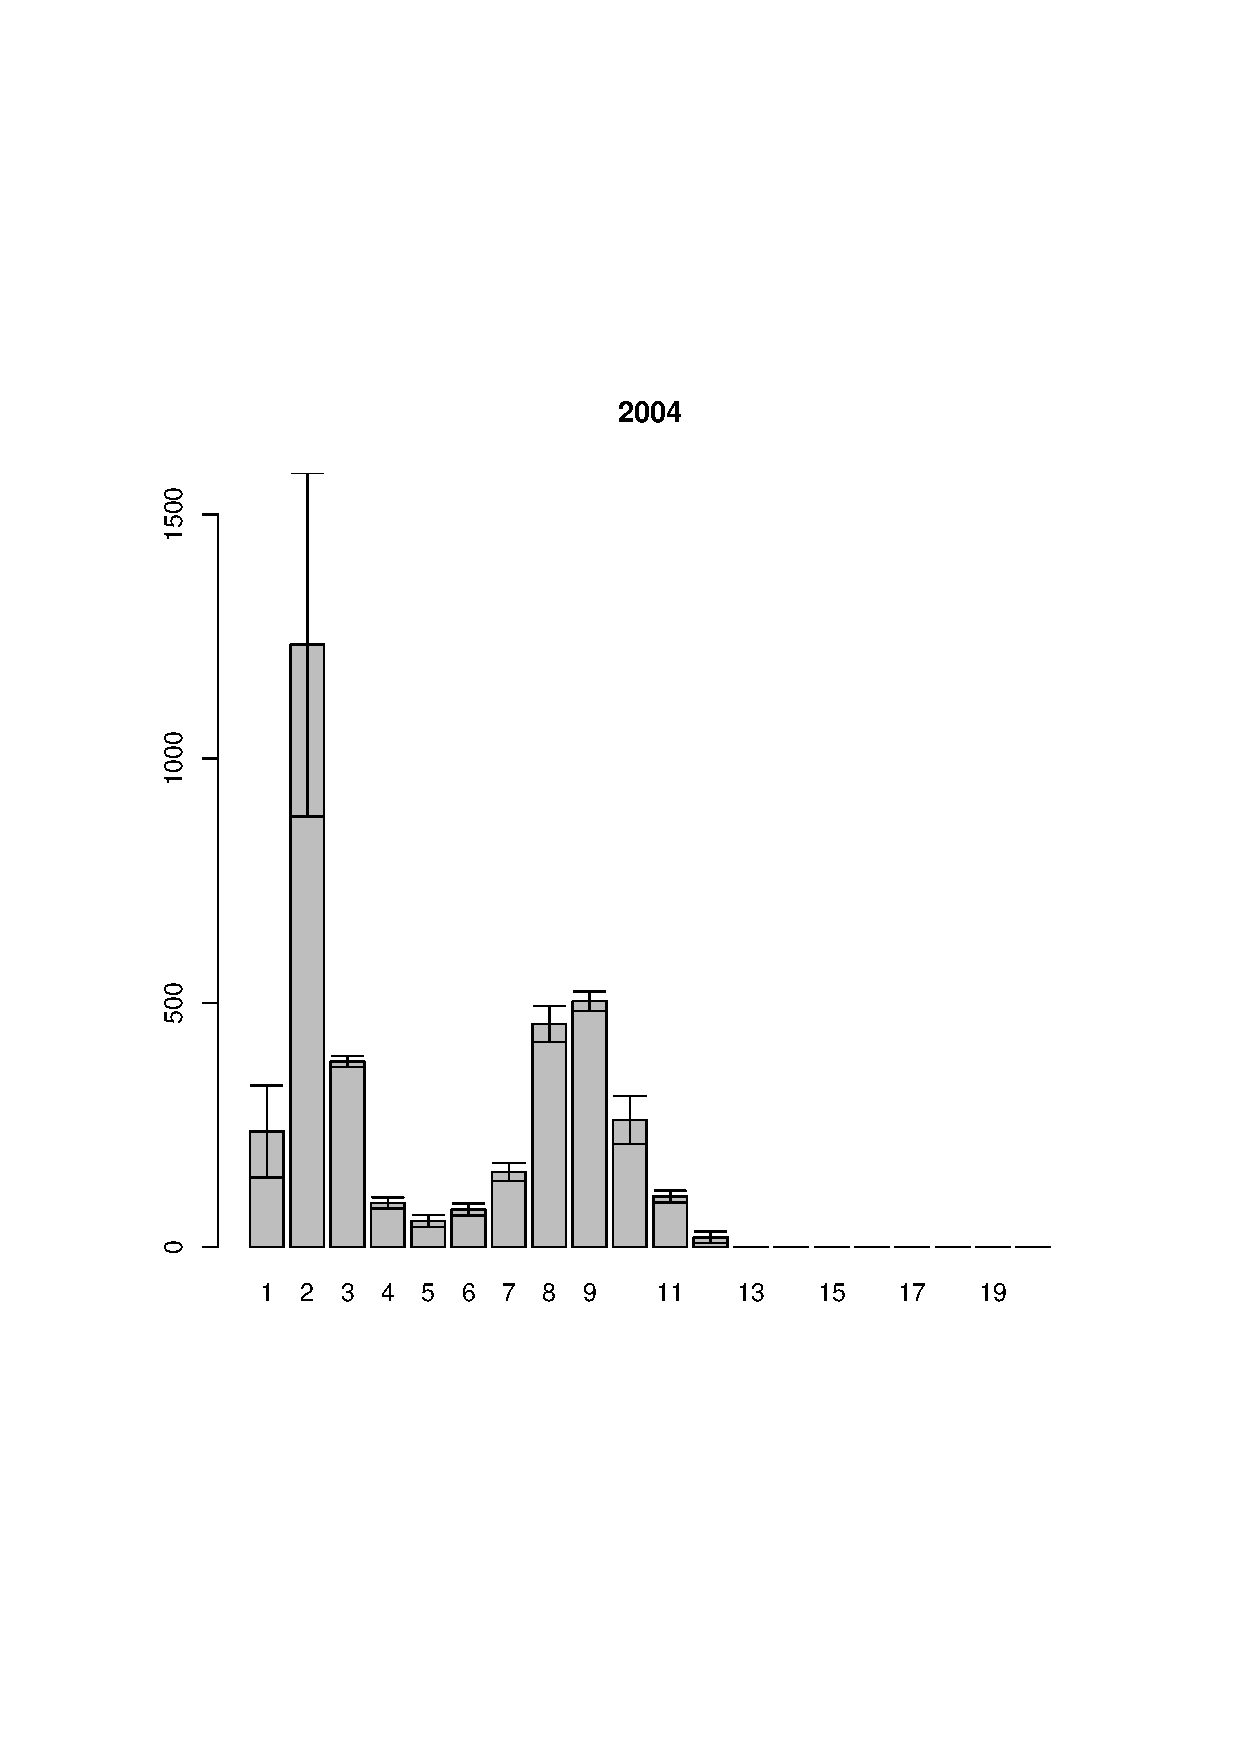
\includegraphics[width=60mm]{../White_Sea/Estuatiy_Luvenga/sizestr_2004_.pdf}
\hfill
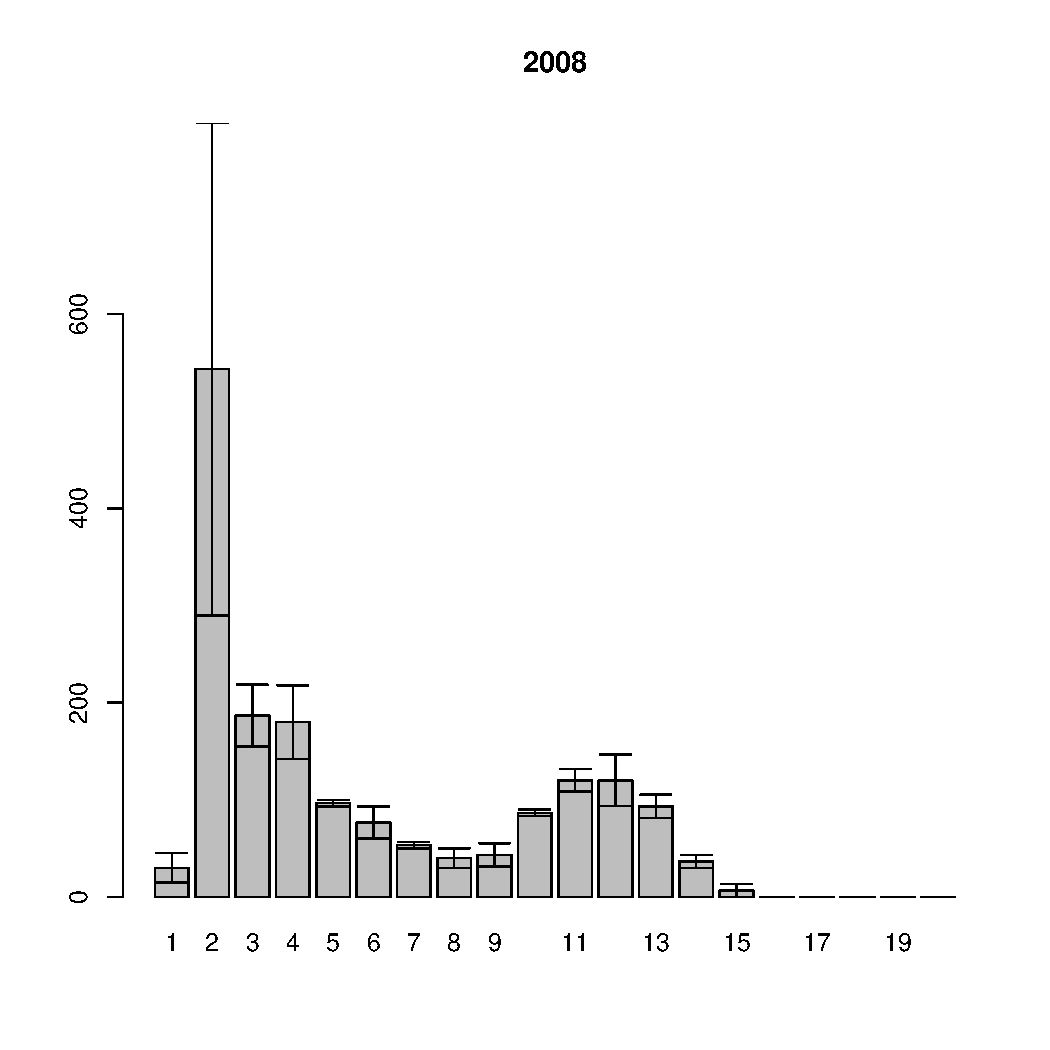
\includegraphics[width=60mm]{../White_Sea/Estuatiy_Luvenga/sizestr_2008_.pdf}
\hfill
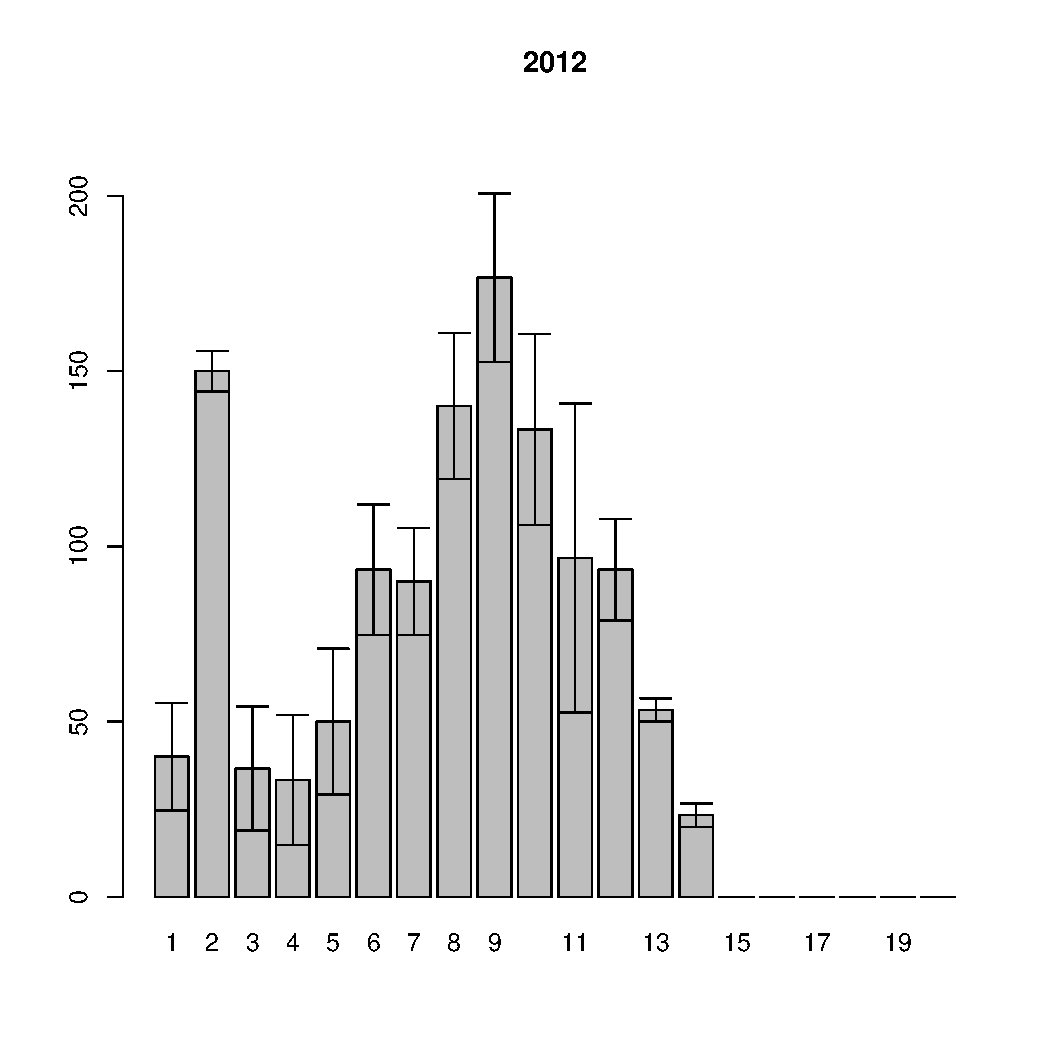
\includegraphics[width=60mm]{../White_Sea/Estuatiy_Luvenga/sizestr_2012_.pdf}
\end{multicols}

%\smallskip


\begin{multicols}{3}
\hfill
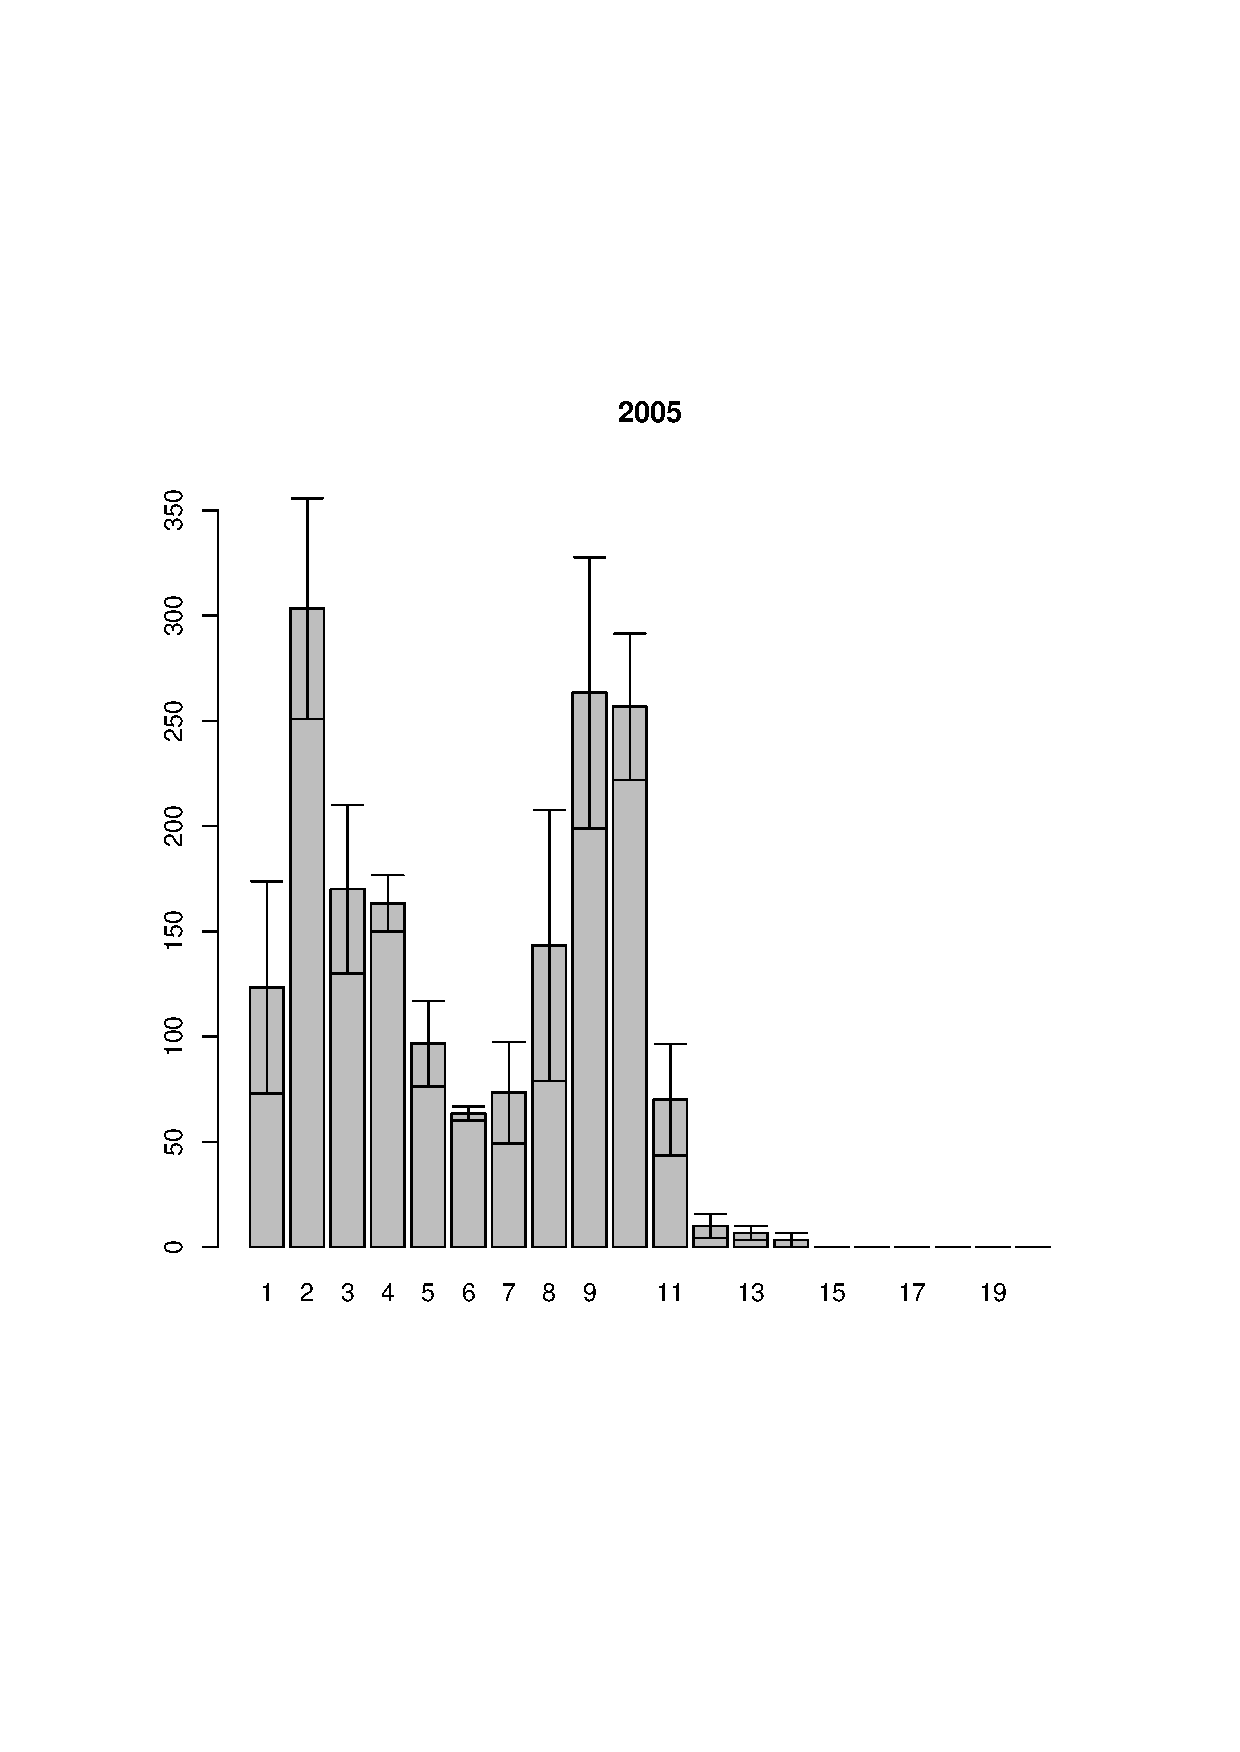
\includegraphics[width=60mm]{../White_Sea/Estuatiy_Luvenga/sizestr_2005_.pdf}
\hfill
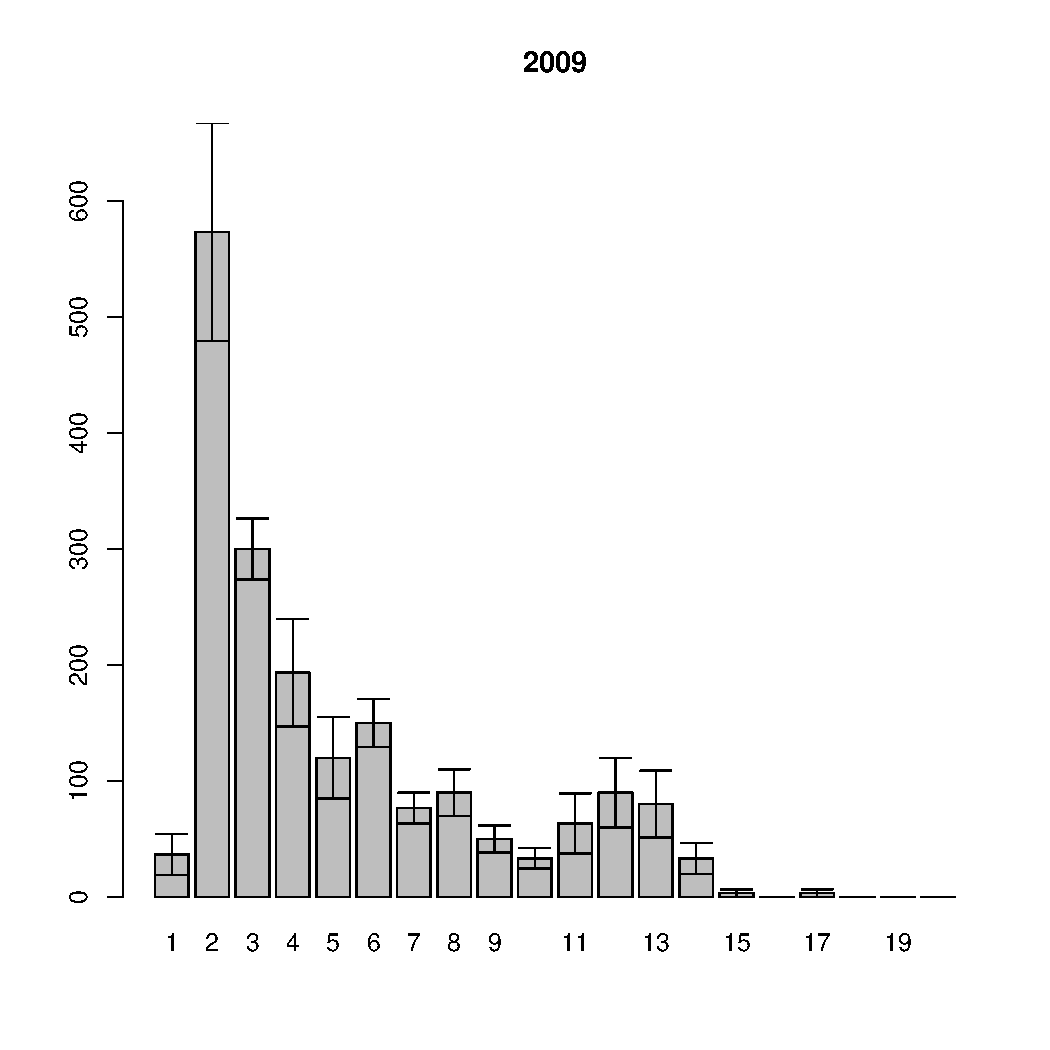
\includegraphics[width=60mm]{../White_Sea/Estuatiy_Luvenga/sizestr_2009_.pdf}
%\hfill
%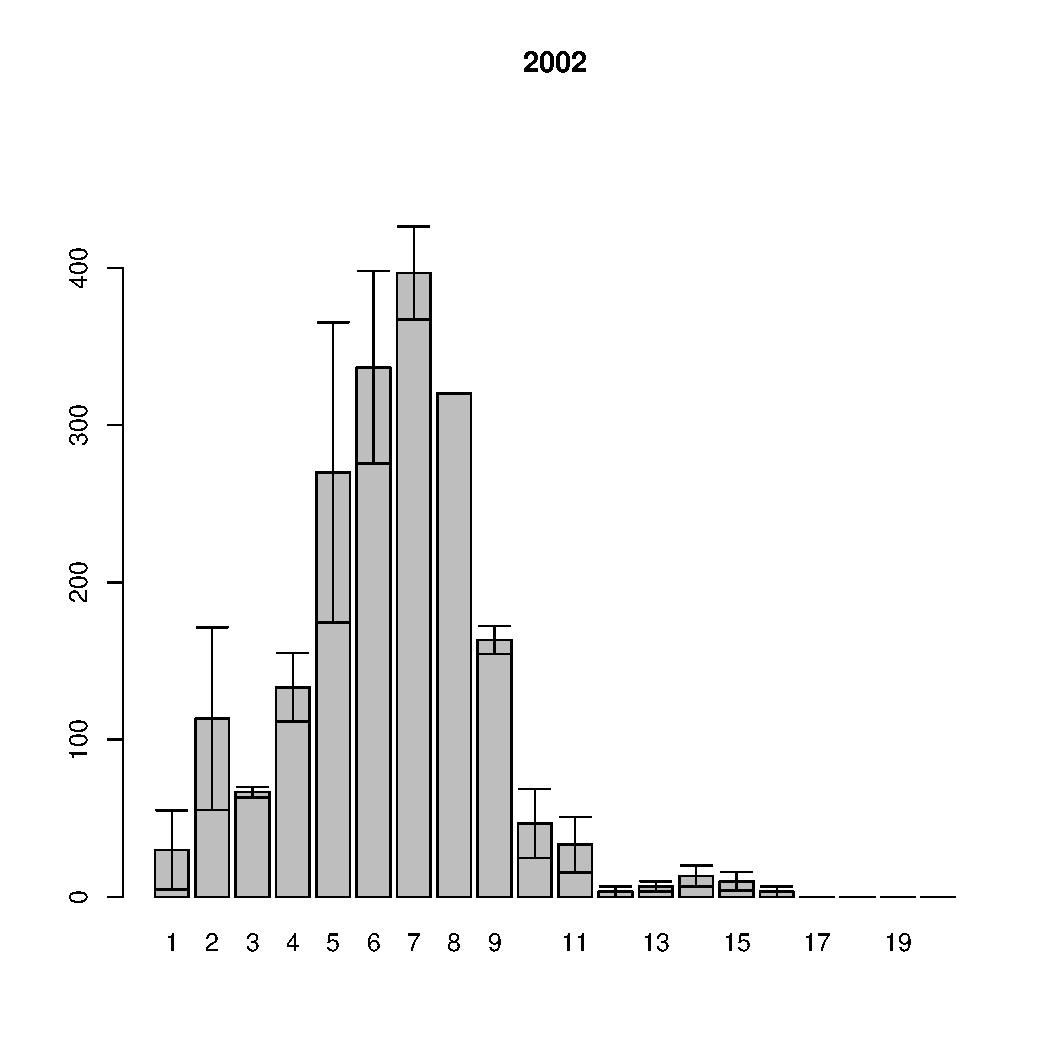
\includegraphics[width=60mm]{../White_Sea/Estuatiy_Luvenga/sizestr_2002_.pdf}
\end{multicols}

%\smallskip

\begin{multicols}{3}
\hfill
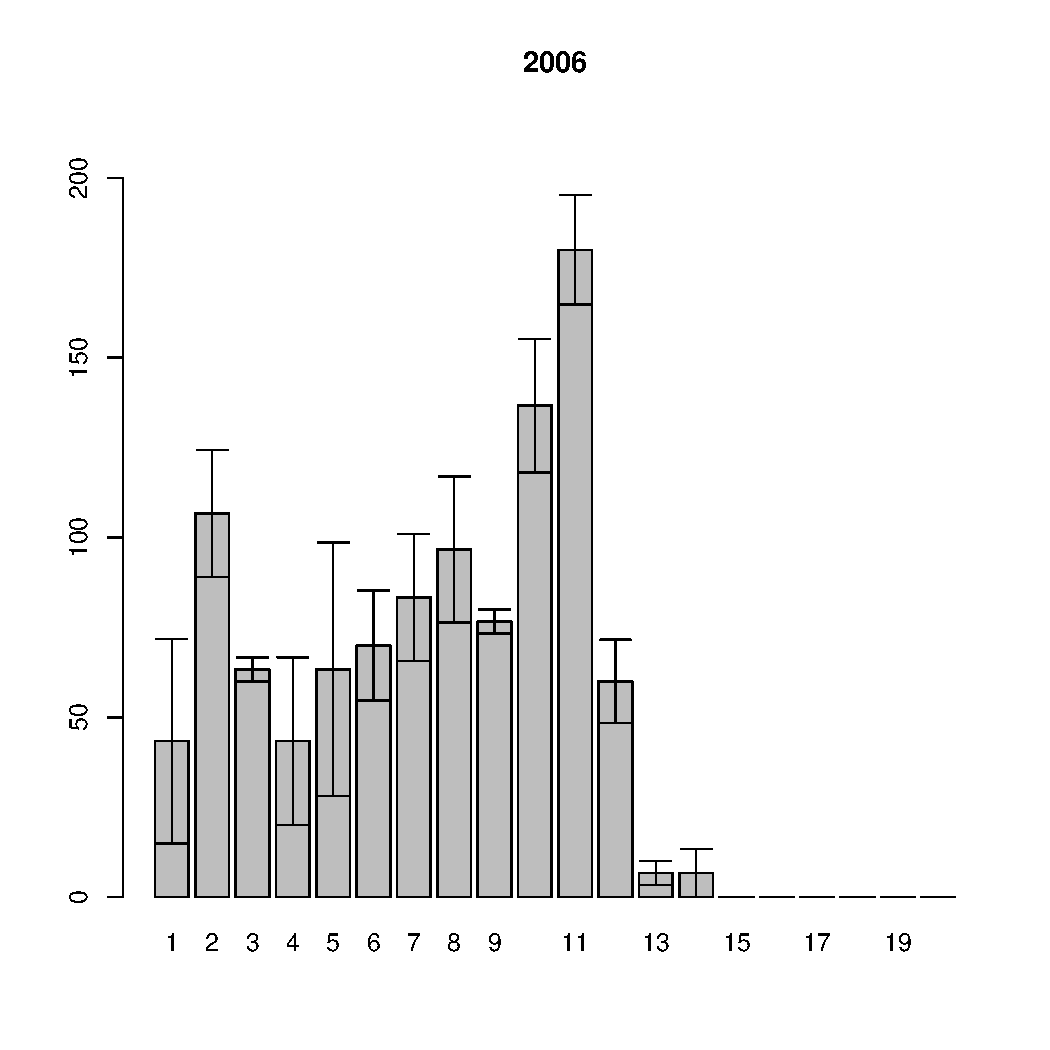
\includegraphics[width=60mm]{../White_Sea/Estuatiy_Luvenga/sizestr_2006_.pdf}
\hfill
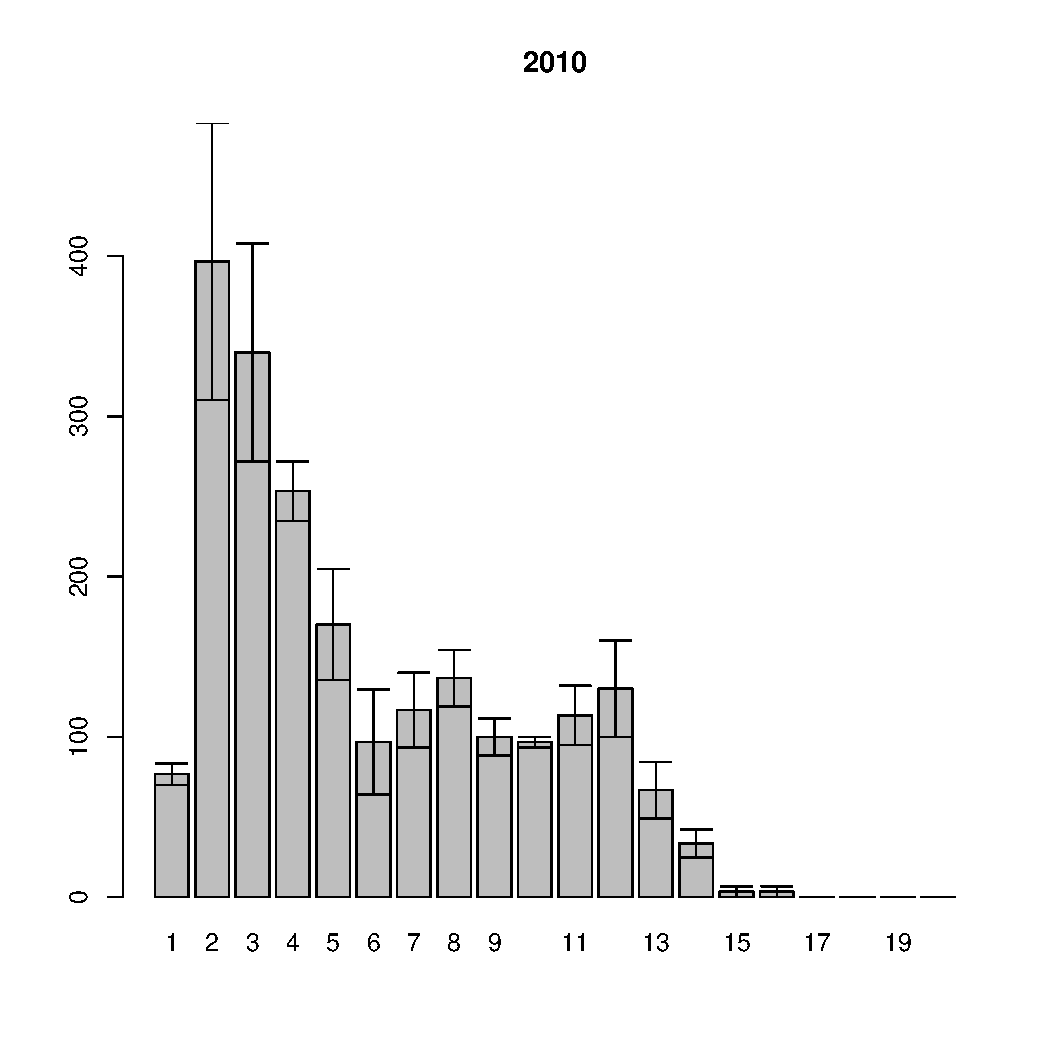
\includegraphics[width=60mm]{../White_Sea/Estuatiy_Luvenga/sizestr_2010_.pdf}
%\hfill
%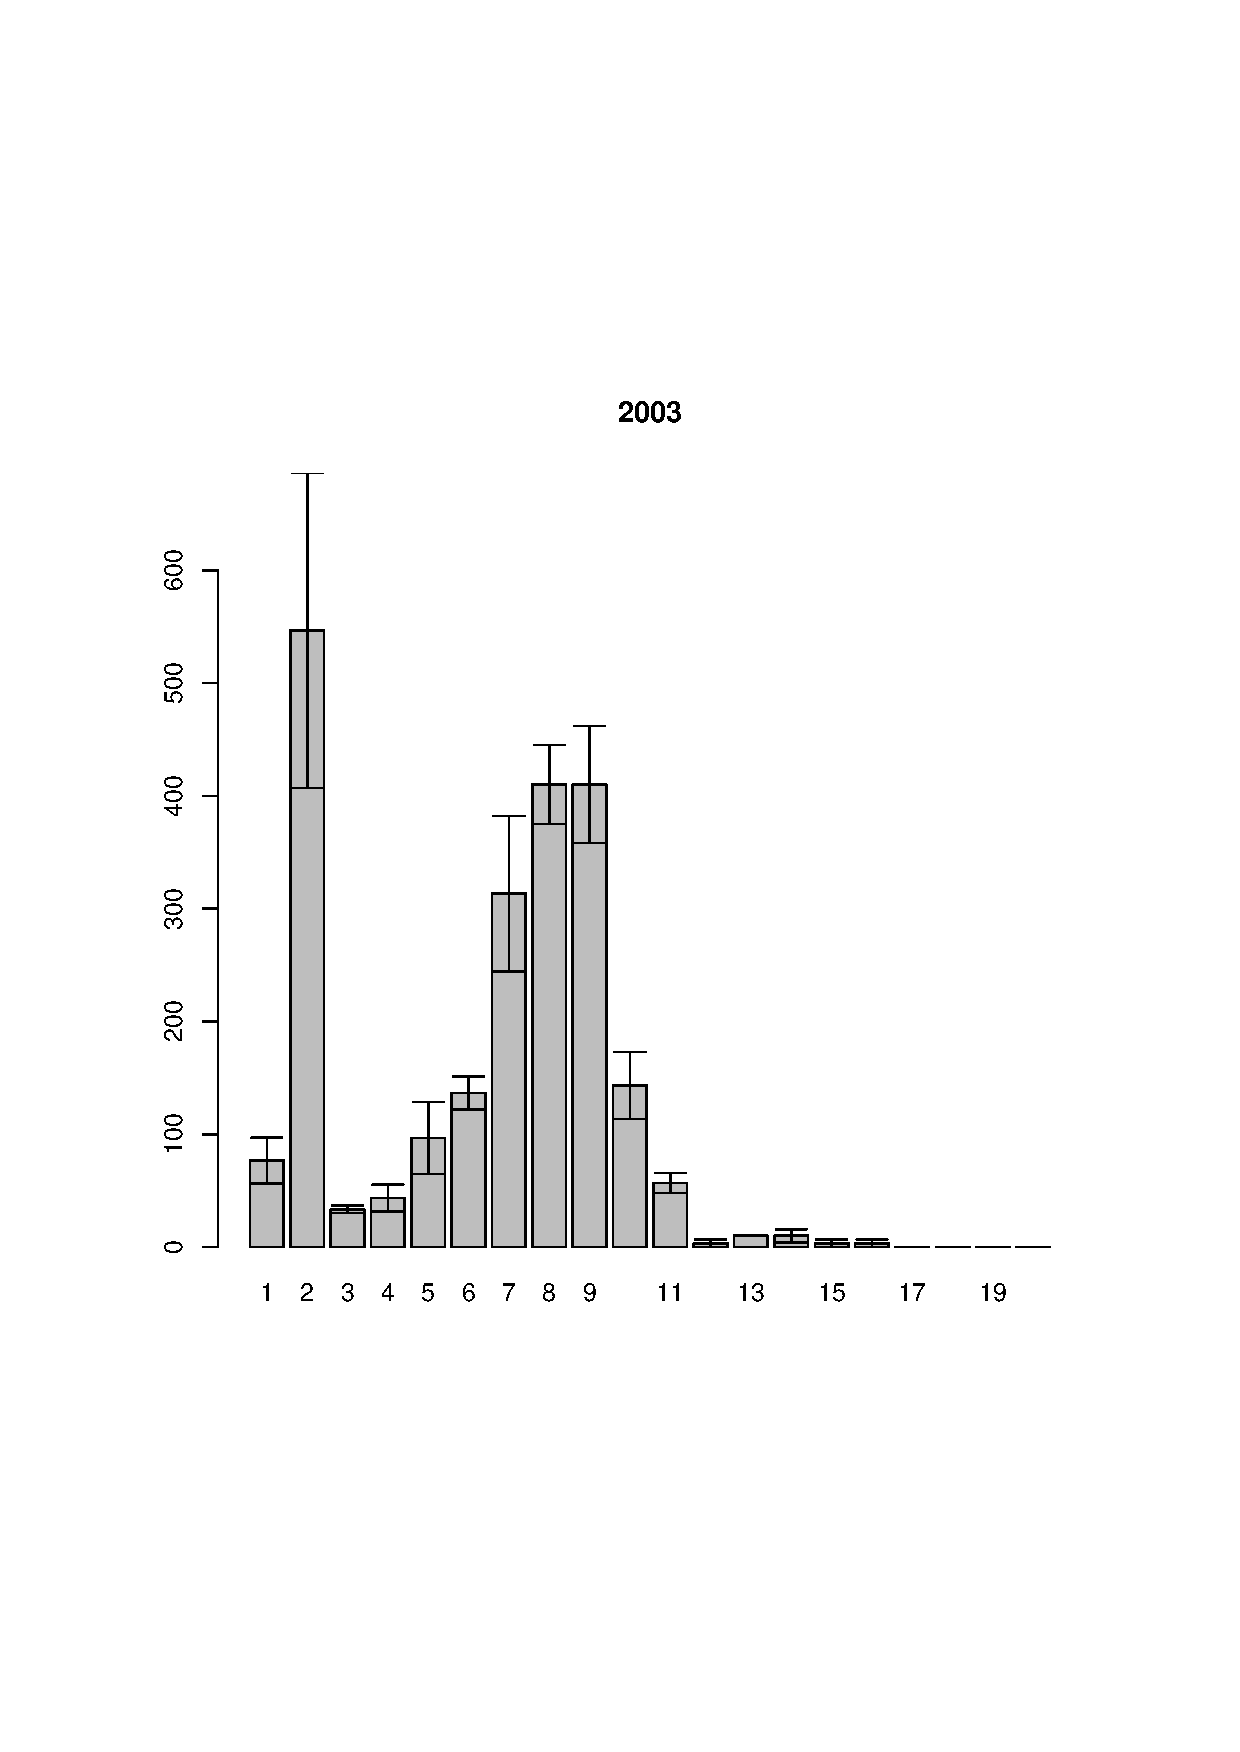
\includegraphics[width=60mm]{../White_Sea/Estuatiy_Luvenga/sizestr_2003_.pdf}
\end{multicols}

%\smallskip

\begin{multicols}{3}
\hfill
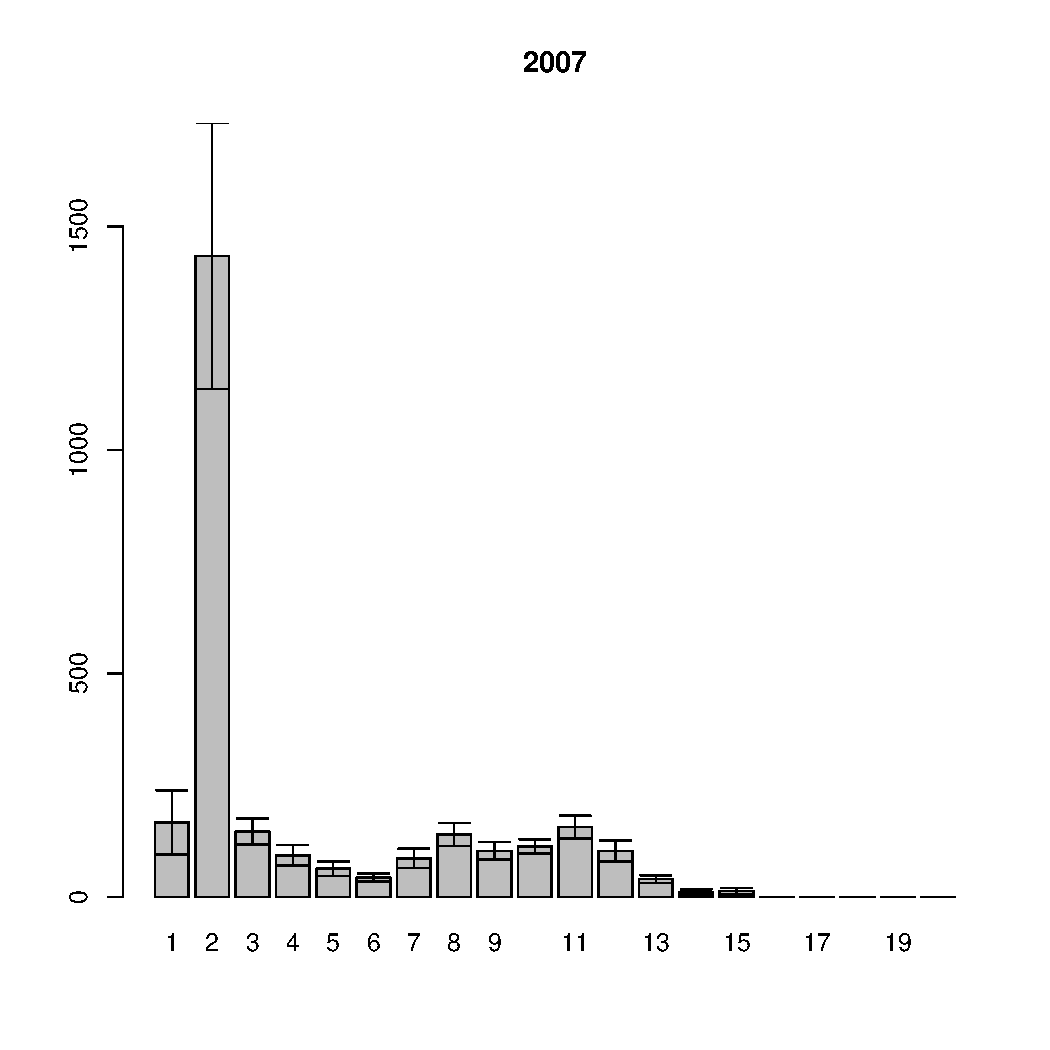
\includegraphics[width=60mm]{../White_Sea/Estuatiy_Luvenga/sizestr_2007_.pdf}
\hfill
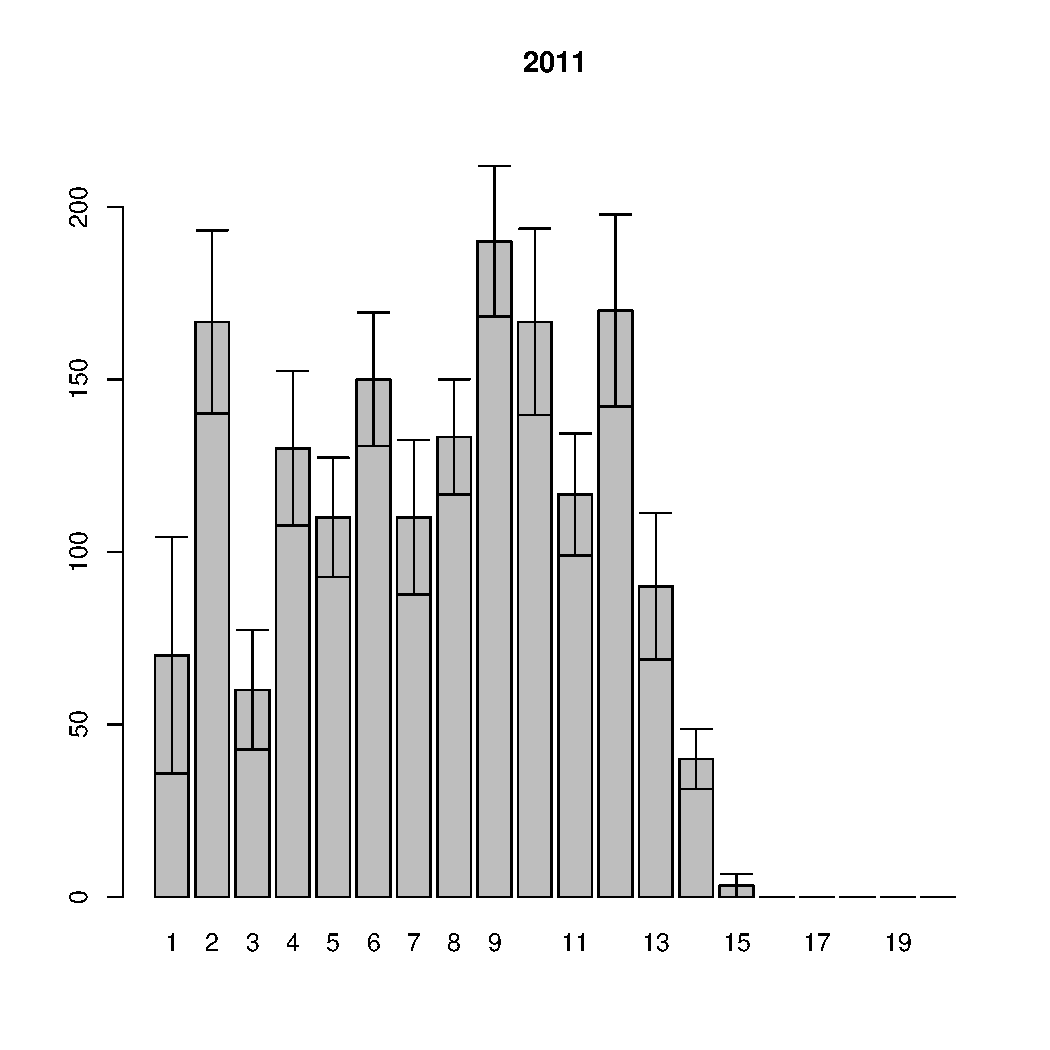
\includegraphics[width=60mm]{../White_Sea/Estuatiy_Luvenga/sizestr_2011_.pdf}
%\hfill
%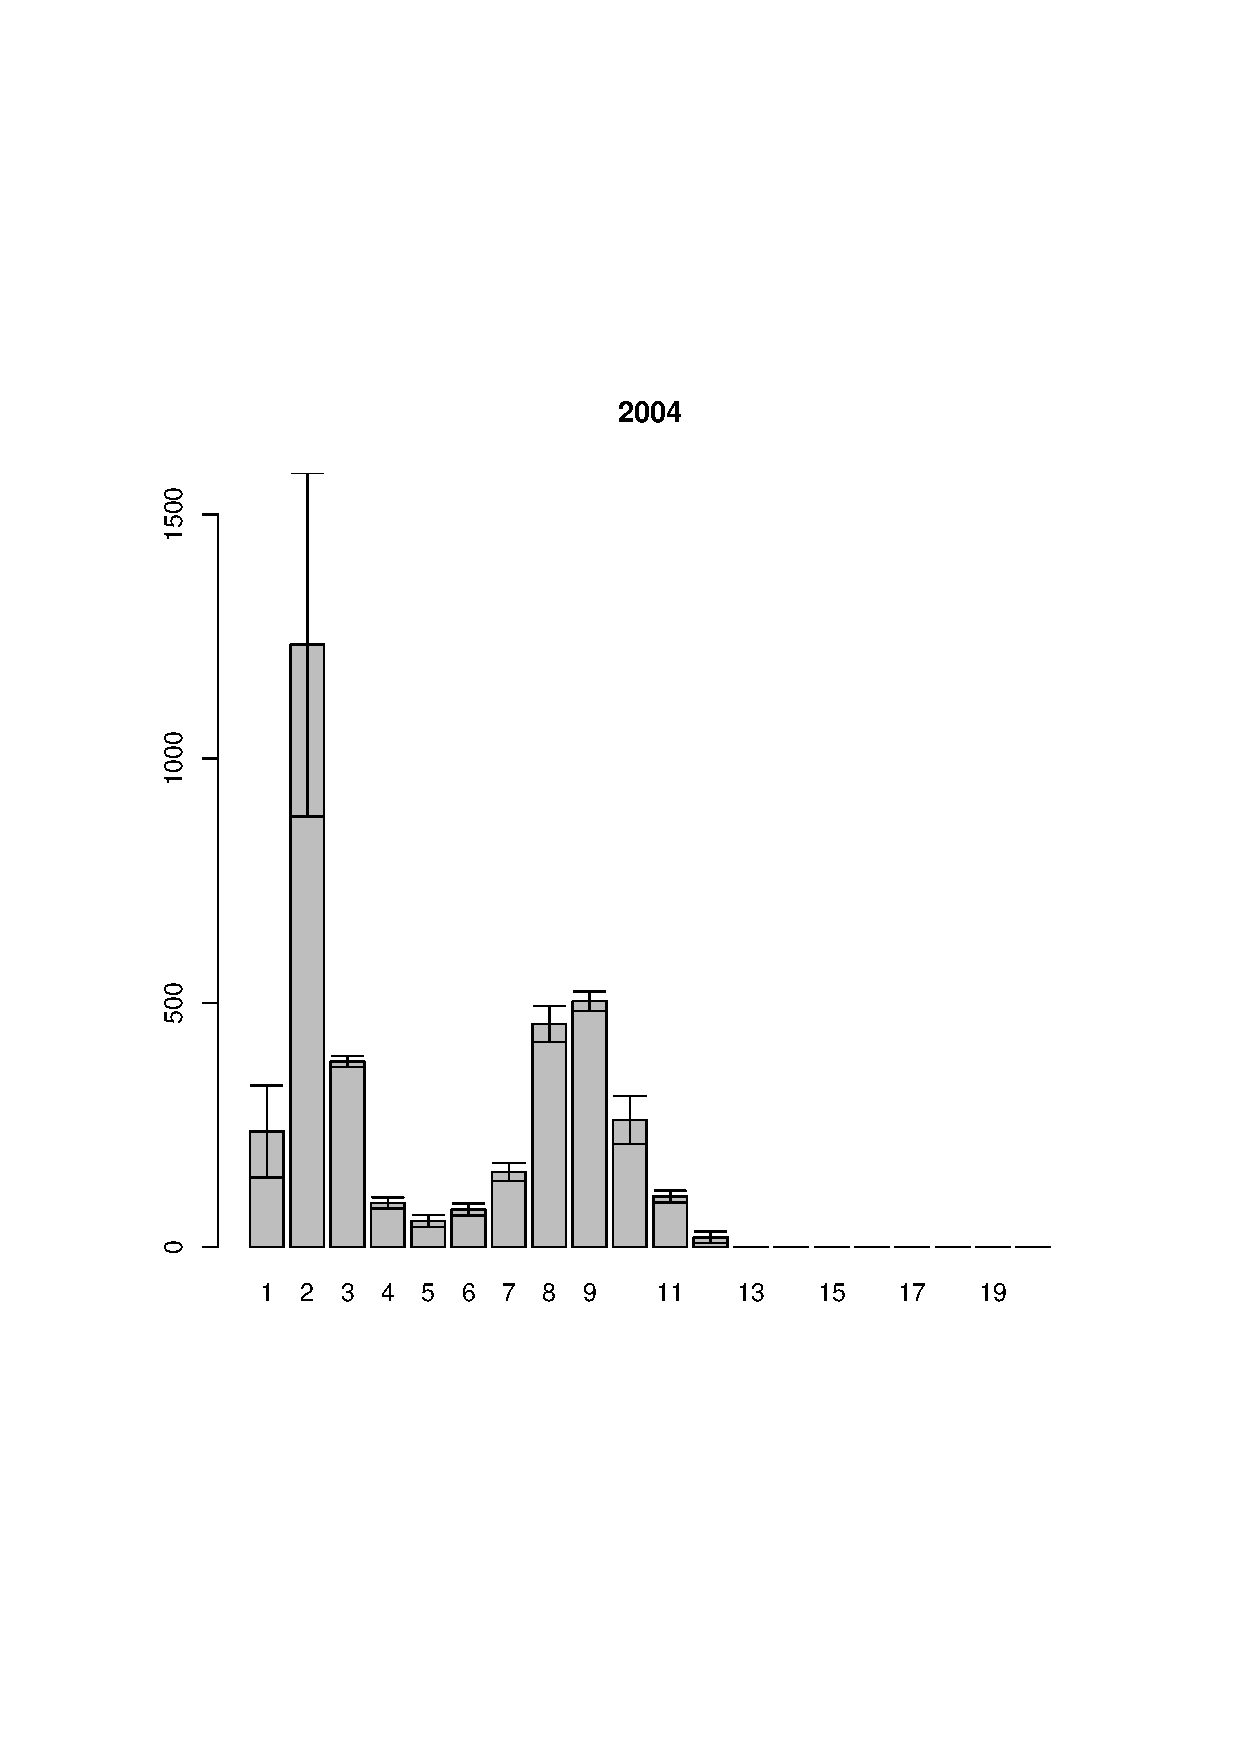
\includegraphics[width=60mm]{../White_Sea/Estuatiy_Luvenga/sizestr_2004_.pdf}
\end{multicols}


%\caption{Размерная структура {\it Macoma balthica} в СГЛ эстуария р. Лувеньги}
%\label{ris:size_str_estuaty_Luv}
\begin{center}
Рис. \ref{ris:size_str_estuary_Luv} (продолжение). Размерная структура {\it Macoma balthica} в СГЛ эстуария р. Лувеньги

\end{center}
\end{figure}

%Горелый Лувеньга
\begin{figure}[h]

\begin{multicols}{3}
\hfill
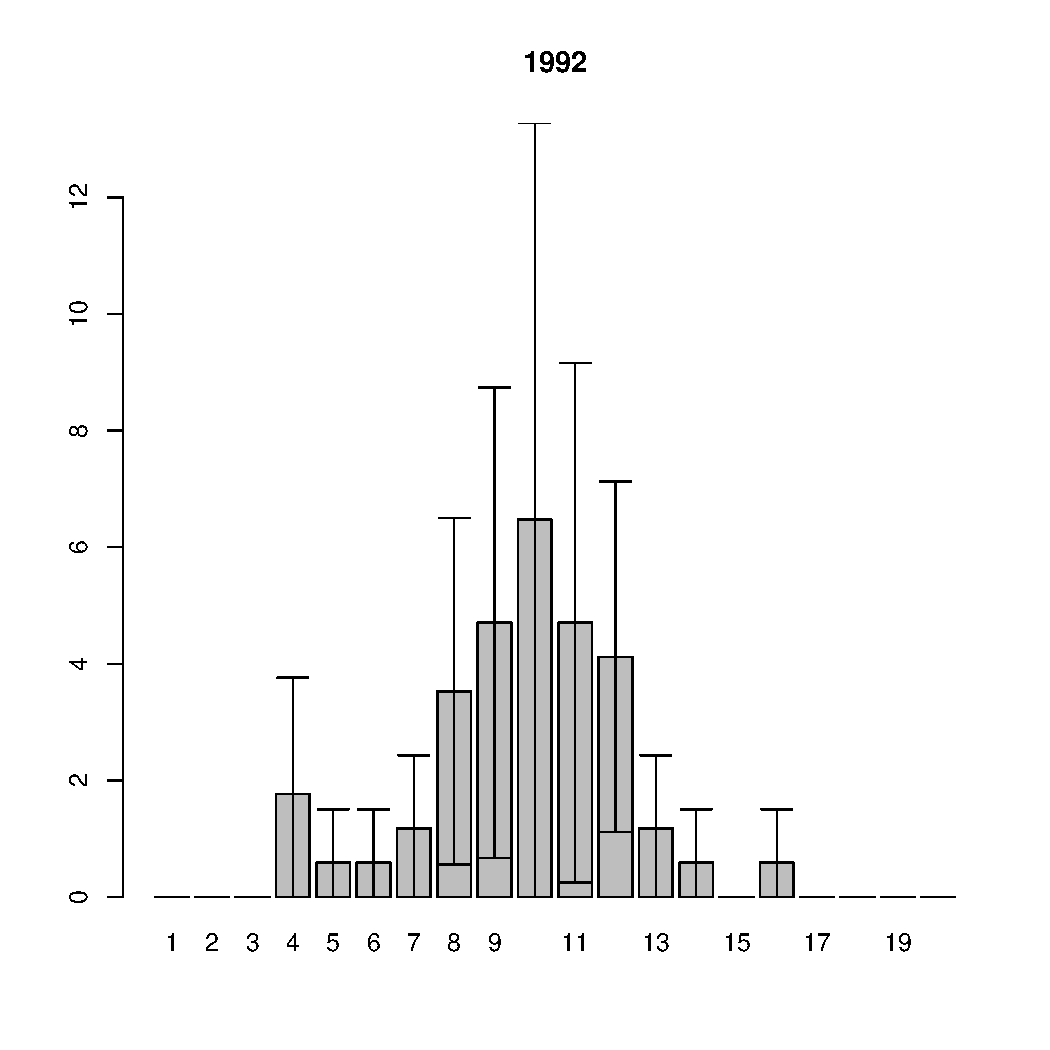
\includegraphics[width=60mm]{../White_Sea/Luvenga_Goreliy/high_1992_.pdf}
\hfill
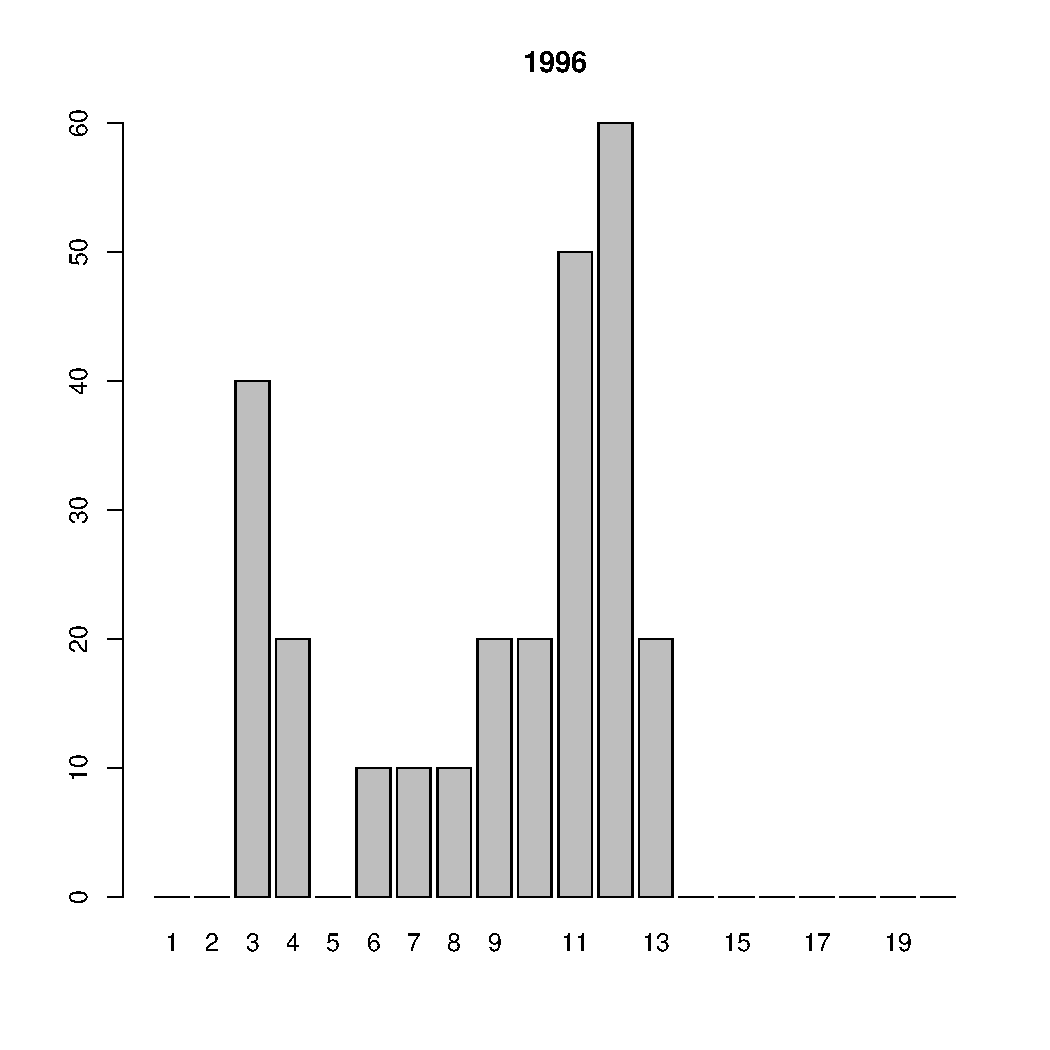
\includegraphics[width=60mm]{../White_Sea/Luvenga_Goreliy/high_1996_.pdf}
\hfill
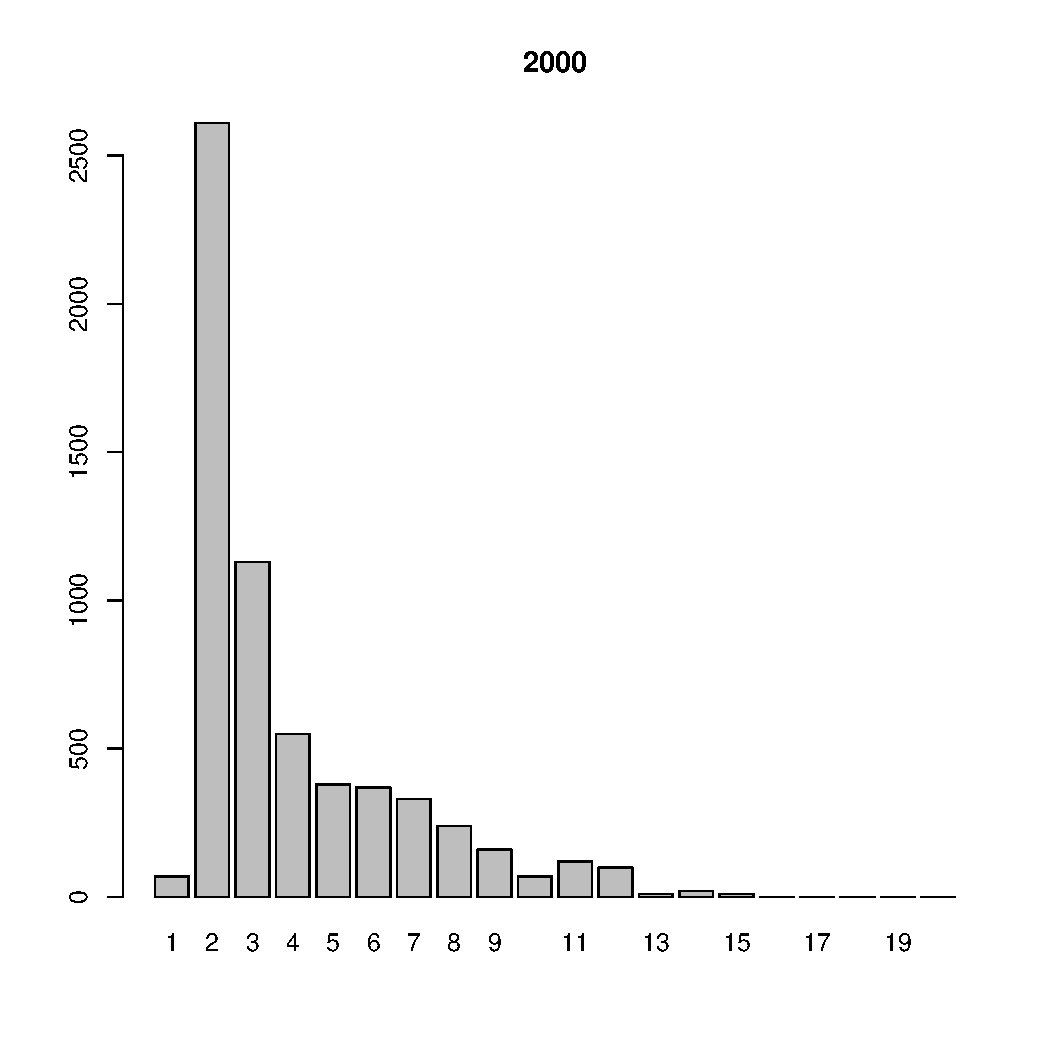
\includegraphics[width=60mm]{../White_Sea/Luvenga_Goreliy/high_2000_.pdf}
\end{multicols}

%\smallskip


\begin{multicols}{3}
\hfill
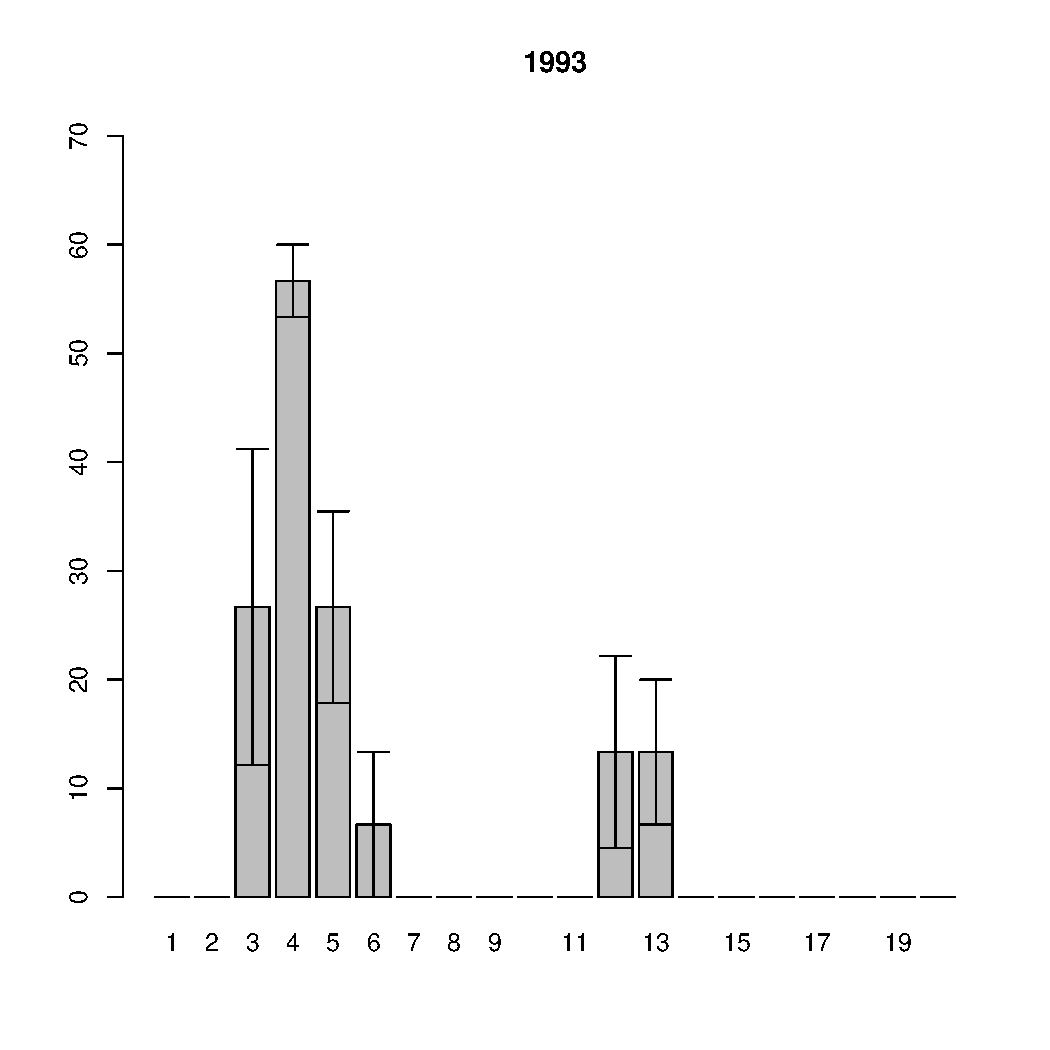
\includegraphics[width=60mm]{../White_Sea/Luvenga_Goreliy/high_1993_.pdf}
\hfill
\includegraphics[width=60mm]{../White_Sea/Luvenga_Goreliy/high_1997_.pdf}
\hfill
\includegraphics[width=60mm]{../White_Sea/Luvenga_Goreliy/high_2001_.pdf}
\end{multicols}

%\smallskip

\begin{multicols}{3}
\hfill
\includegraphics[width=60mm]{../White_Sea/Luvenga_Goreliy/high_1994_.pdf}
\hfill
\includegraphics[width=60mm]{../White_Sea/Luvenga_Goreliy/high_1998_.pdf}
\hfill
\includegraphics[width=60mm]{../White_Sea/Luvenga_Goreliy/high_2002_.pdf}
\end{multicols}

%\smallskip

\begin{multicols}{3}
\hfill
\includegraphics[width=60mm]{../White_Sea/Luvenga_Goreliy/high_1995_.pdf}
\hfill
\includegraphics[width=60mm]{../White_Sea/Luvenga_Goreliy/high_1999_.pdf}
\hfill
\includegraphics[width=60mm]{../White_Sea/Luvenga_Goreliy/high_2003_.pdf}
\end{multicols}


\caption{Размерная структура {\it Macoma balthica} в ВГЛ о. Горелого}
\label{ris:size_str_Goreliy_high}
\end{figure}


\begin{figure}[h]

\begin{multicols}{3}
\hfill
\includegraphics[width=60mm]{../White_Sea/Luvenga_Goreliy/high_2004_.pdf}
\hfill
\includegraphics[width=60mm]{../White_Sea/Luvenga_Goreliy/high_2008_.pdf}
\hfill
\includegraphics[width=60mm]{../White_Sea/Luvenga_Goreliy/high_2012_.pdf}
\end{multicols}

%\smallskip


\begin{multicols}{3}
\hfill
\includegraphics[width=60mm]{../White_Sea/Luvenga_Goreliy/high_2005_.pdf}
\hfill
\includegraphics[width=60mm]{../White_Sea/Luvenga_Goreliy/high_2009_.pdf}
%\hfill
%\includegraphics[width=60mm]{../White_Sea/Luvenga_Goreliy/high_2002_.pdf}
\end{multicols}

%\smallskip

\begin{multicols}{3}
\hfill
\includegraphics[width=60mm]{../White_Sea/Luvenga_Goreliy/high_2006_.pdf}
\hfill
\includegraphics[width=60mm]{../White_Sea/Luvenga_Goreliy/high_2010_.pdf}
%\hfill
%\includegraphics[width=60mm]{../White_Sea/Luvenga_Goreliy/high_2003_.pdf}
\end{multicols}

%\smallskip

\begin{multicols}{3}
\hfill
\includegraphics[width=60mm]{../White_Sea/Luvenga_Goreliy/high_2007_.pdf}
\hfill
\includegraphics[width=60mm]{../White_Sea/Luvenga_Goreliy/high_2011_.pdf}
%\hfill
%\includegraphics[width=60mm]{../White_Sea/Luvenga_Goreliy/high_2004_.pdf}
\end{multicols}


%\caption{Размерная структура {\it Macoma balthica} в СГЛ эстуария р. Лувеньги}
%\label{ris:size_str_estuaty_Luv}
\begin{center}
Рис. \ref{ris:size_str_Goreliy_high} (продолжение). Размерная структура {\it Macoma balthica} в ВГЛ о. Горелого

\end{center}
\end{figure}

% Горелый СГЛ
\begin{figure}[h]

\begin{multicols}{3}
\hfill
\includegraphics[width=60mm]{../White_Sea/Luvenga_Goreliy/middle_1992_.pdf}
\hfill
\includegraphics[width=60mm]{../White_Sea/Luvenga_Goreliy/middle_1996_.pdf}
\hfill
\includegraphics[width=60mm]{../White_Sea/Luvenga_Goreliy/middle_2000_.pdf}
\end{multicols}

%\smallskip


\begin{multicols}{3}
\hfill
\includegraphics[width=60mm]{../White_Sea/Luvenga_Goreliy/middle_1993_.pdf}
\hfill
\includegraphics[width=60mm]{../White_Sea/Luvenga_Goreliy/middle_1997_.pdf}
\hfill
\includegraphics[width=60mm]{../White_Sea/Luvenga_Goreliy/middle_2001_.pdf}
\end{multicols}

%\smallskip

\begin{multicols}{3}
\hfill
\includegraphics[width=60mm]{../White_Sea/Luvenga_Goreliy/middle_1994_.pdf}
\hfill
\includegraphics[width=60mm]{../White_Sea/Luvenga_Goreliy/middle_1998_.pdf}
\hfill
\includegraphics[width=60mm]{../White_Sea/Luvenga_Goreliy/middle_2002_.pdf}
\end{multicols}

%\smallskip

\begin{multicols}{3}
\hfill
\includegraphics[width=60mm]{../White_Sea/Luvenga_Goreliy/middle_1995_.pdf}
\hfill
\includegraphics[width=60mm]{../White_Sea/Luvenga_Goreliy/middle_1999_.pdf}
\hfill
\includegraphics[width=60mm]{../White_Sea/Luvenga_Goreliy/middle_2003_.pdf}
\end{multicols}


\caption{Размерная структура {\it Macoma balthica} в СГЛ о. Горелого}
\label{ris:size_str_Goreliy_mid}
\end{figure}


\begin{figure}[h]

\begin{multicols}{3}
\hfill
\includegraphics[width=60mm]{../White_Sea/Luvenga_Goreliy/middle_2004_.pdf}
\hfill
\includegraphics[width=60mm]{../White_Sea/Luvenga_Goreliy/middle_2008_.pdf}
\hfill
\includegraphics[width=60mm]{../White_Sea/Luvenga_Goreliy/middle_2012_.pdf}
\end{multicols}

%\smallskip


\begin{multicols}{3}
\hfill
\includegraphics[width=60mm]{../White_Sea/Luvenga_Goreliy/middle_2005_.pdf}
\hfill
\includegraphics[width=60mm]{../White_Sea/Luvenga_Goreliy/middle_2009_.pdf}
%\hfill
%\includegraphics[width=60mm]{../White_Sea/Luvenga_Goreliy/middle_2002_.pdf}
\end{multicols}

%\smallskip

\begin{multicols}{3}
\hfill
\includegraphics[width=60mm]{../White_Sea/Luvenga_Goreliy/middle_2006_.pdf}
\hfill
\includegraphics[width=60mm]{../White_Sea/Luvenga_Goreliy/middle_2010_.pdf}
%\hfill
%\includegraphics[width=60mm]{../White_Sea/Luvenga_Goreliy/middle_2003_.pdf}
\end{multicols}

%\smallskip

\begin{multicols}{3}
\hfill
\includegraphics[width=60mm]{../White_Sea/Luvenga_Goreliy/middle_2007_.pdf}
\hfill
\includegraphics[width=60mm]{../White_Sea/Luvenga_Goreliy/middle_2011_.pdf}
%\hfill
%\includegraphics[width=60mm]{../White_Sea/Luvenga_Goreliy/middle_2004_.pdf}
\end{multicols}


%\caption{Размерная структура {\it Macoma balthica} в СГЛ эстуария р. Лувеньги}
%\label{ris:size_str_estuaty_Luv}
\begin{center}
Рис. \ref{ris:size_str_Goreliy_mid} (продолжение). Размерная структура {\it Macoma balthica} в СГЛ о. Горелого

\end{center}
\end{figure}

% Горелый midlow


\begin{figure}[h]

\begin{multicols}{3}
\hfill
\includegraphics[width=60mm]{../White_Sea/Luvenga_Goreliy/midlow_1992_.pdf}
\hfill
\includegraphics[width=60mm]{../White_Sea/Luvenga_Goreliy/midlow_1996_.pdf}
\hfill
\includegraphics[width=60mm]{../White_Sea/Luvenga_Goreliy/midlow_2000_.pdf}
\end{multicols}

%\smallskip


\begin{multicols}{3}
\hfill
\includegraphics[width=60mm]{../White_Sea/Luvenga_Goreliy/midlow_1993_.pdf}
\hfill
\includegraphics[width=60mm]{../White_Sea/Luvenga_Goreliy/midlow_1997_.pdf}
\hfill
\includegraphics[width=60mm]{../White_Sea/Luvenga_Goreliy/midlow_2001_.pdf}
\end{multicols}

%\smallskip

\begin{multicols}{3}
\hfill
\includegraphics[width=60mm]{../White_Sea/Luvenga_Goreliy/midlow_1994_.pdf}
\hfill
\includegraphics[width=60mm]{../White_Sea/Luvenga_Goreliy/midlow_1998_.pdf}
\hfill
\includegraphics[width=60mm]{../White_Sea/Luvenga_Goreliy/midlow_2002_.pdf}
\end{multicols}

%\smallskip

\begin{multicols}{3}
\hfill
\includegraphics[width=60mm]{../White_Sea/Luvenga_Goreliy/midlow_1995_.pdf}
\hfill
\includegraphics[width=60mm]{../White_Sea/Luvenga_Goreliy/midlow_1999_.pdf}
\hfill
\includegraphics[width=60mm]{../White_Sea/Luvenga_Goreliy/midlow_2003_.pdf}
\end{multicols}


\caption{Размерная структура {\it Macoma balthica} в поясе фукоидов о. Горелого}
\label{ris:size_str_Goreliy_midlow}
\end{figure}


\begin{figure}[h]

\begin{multicols}{3}
\hfill
\includegraphics[width=60mm]{../White_Sea/Luvenga_Goreliy/midlow_2004_.pdf}
\hfill
\includegraphics[width=60mm]{../White_Sea/Luvenga_Goreliy/midlow_2008_.pdf}
\hfill
\includegraphics[width=60mm]{../White_Sea/Luvenga_Goreliy/midlow_2012_.pdf}
\end{multicols}

%\smallskip


\begin{multicols}{3}
\hfill
\includegraphics[width=60mm]{../White_Sea/Luvenga_Goreliy/midlow_2005_.pdf}
\hfill
\includegraphics[width=60mm]{../White_Sea/Luvenga_Goreliy/midlow_2009_.pdf}
%\hfill
%\includegraphics[width=60mm]{../White_Sea/Luvenga_Goreliy/midlow_2002_.pdf}
\end{multicols}

%\smallskip

\begin{multicols}{3}
\hfill
\includegraphics[width=60mm]{../White_Sea/Luvenga_Goreliy/midlow_2006_.pdf}
\hfill
\includegraphics[width=60mm]{../White_Sea/Luvenga_Goreliy/midlow_2010_.pdf}
%\hfill
%\includegraphics[width=60mm]{../White_Sea/Luvenga_Goreliy/midlow_2003_.pdf}
\end{multicols}

%\smallskip

\begin{multicols}{3}
\hfill
\includegraphics[width=60mm]{../White_Sea/Luvenga_Goreliy/midlow_2007_.pdf}
\hfill
\includegraphics[width=60mm]{../White_Sea/Luvenga_Goreliy/midlow_2011_.pdf}
%\hfill
%\includegraphics[width=60mm]{../White_Sea/Luvenga_Goreliy/midlow_2004_.pdf}
\end{multicols}


%\caption{Размерная структура {\it Macoma balthica} в СГЛ эстуария р. Лувеньги}
%\label{ris:size_str_estuaty_Luv}
\begin{center}
Рис. \ref{ris:size_str_Goreliy_midlow} (продолжение). Размерная структура {\it Macoma balthica} в поясе фукоидов о. Горелого

\end{center}
\end{figure}


% Горелый НГЛ
\begin{figure}[h]

\begin{multicols}{3}
\hfill
\includegraphics[width=60mm]{../White_Sea/Luvenga_Goreliy/low_1992_.pdf}
\hfill
\includegraphics[width=60mm]{../White_Sea/Luvenga_Goreliy/low_1996_.pdf}
\hfill
\includegraphics[width=60mm]{../White_Sea/Luvenga_Goreliy/low_2000_.pdf}
\end{multicols}

%\smallskip


\begin{multicols}{3}
\hfill
\includegraphics[width=60mm]{../White_Sea/Luvenga_Goreliy/low_1993_.pdf}
\hfill
\includegraphics[width=60mm]{../White_Sea/Luvenga_Goreliy/low_1997_.pdf}
\hfill
\includegraphics[width=60mm]{../White_Sea/Luvenga_Goreliy/low_2001_.pdf}
\end{multicols}

%\smallskip

\begin{multicols}{3}
\hfill
\includegraphics[width=60mm]{../White_Sea/Luvenga_Goreliy/low_1994_.pdf}
\hfill
\includegraphics[width=60mm]{../White_Sea/Luvenga_Goreliy/low_1998_.pdf}
\hfill
\includegraphics[width=60mm]{../White_Sea/Luvenga_Goreliy/low_2002_.pdf}
\end{multicols}

%\smallskip

\begin{multicols}{3}
\hfill
\includegraphics[width=60mm]{../White_Sea/Luvenga_Goreliy/low_1995_.pdf}
\hfill
\includegraphics[width=60mm]{../White_Sea/Luvenga_Goreliy/low_1999_.pdf}
\hfill
\includegraphics[width=60mm]{../White_Sea/Luvenga_Goreliy/low_2003_.pdf}
\end{multicols}


\caption{Размерная структура {\it Macoma balthica} в НГЛ о. Горелого}
\label{ris:size_str_Goreliy_low}
\end{figure}


\begin{figure}[h]

\begin{multicols}{3}
\hfill
\includegraphics[width=60mm]{../White_Sea/Luvenga_Goreliy/low_2004_.pdf}
\hfill
\includegraphics[width=60mm]{../White_Sea/Luvenga_Goreliy/low_2008_.pdf}
\hfill
\includegraphics[width=60mm]{../White_Sea/Luvenga_Goreliy/low_2012_.pdf}
\end{multicols}

%\smallskip


\begin{multicols}{3}
\hfill
\includegraphics[width=60mm]{../White_Sea/Luvenga_Goreliy/low_2005_.pdf}
\hfill
\includegraphics[width=60mm]{../White_Sea/Luvenga_Goreliy/low_2009_.pdf}
%\hfill
%\includegraphics[width=60mm]{../White_Sea/Luvenga_Goreliy/low_2002_.pdf}
\end{multicols}

%\smallskip

\begin{multicols}{3}
\hfill
\includegraphics[width=60mm]{../White_Sea/Luvenga_Goreliy/low_2006_.pdf}
\hfill
\includegraphics[width=60mm]{../White_Sea/Luvenga_Goreliy/low_2010_.pdf}
%\hfill
%\includegraphics[width=60mm]{../White_Sea/Luvenga_Goreliy/low_2003_.pdf}
\end{multicols}

%\smallskip

\begin{multicols}{3}
\hfill
\includegraphics[width=60mm]{../White_Sea/Luvenga_Goreliy/low_2007_.pdf}
\hfill
\includegraphics[width=60mm]{../White_Sea/Luvenga_Goreliy/low_2011_.pdf}
%\hfill
%\includegraphics[width=60mm]{../White_Sea/Luvenga_Goreliy/low_2004_.pdf}
\end{multicols}


%\caption{Размерная структура {\it Macoma balthica} в СГЛ эстуария р. Лувеньги}
%\label{ris:size_str_estuaty_Luv}
\begin{center}
Рис. \ref{ris:size_str_Goreliy_low} (продолжение). Размерная структура {\it Macoma balthica} в НГЛ
 о. Горелого

\end{center}
\end{figure}


%II разрез high

\begin{figure}[h]

\begin{multicols}{3}
\hfill
\includegraphics[width=60mm]{../White_Sea/Luvenga_II_razrez/high_beatch_1992_.pdf}
\hfill
\includegraphics[width=60mm]{../White_Sea/Luvenga_II_razrez/high_beatch_1996_.pdf}
\hfill
\includegraphics[width=60mm]{../White_Sea/Luvenga_II_razrez/high_beatch_2000_.pdf}
\end{multicols}

%\smallskip


\begin{multicols}{3}
\hfill
\includegraphics[width=60mm]{../White_Sea/Luvenga_II_razrez/high_beatch_1993_.pdf}
\hfill
\includegraphics[width=60mm]{../White_Sea/Luvenga_II_razrez/high_beatch_1997_.pdf}
\hfill
\includegraphics[width=60mm]{../White_Sea/Luvenga_II_razrez/high_beatch_2002_.pdf}
\end{multicols}

%\smallskip

\begin{multicols}{3}
\hfill
\includegraphics[width=60mm]{../White_Sea/Luvenga_II_razrez/high_beatch_1994_.pdf}
\hfill
\includegraphics[width=60mm]{../White_Sea/Luvenga_II_razrez/high_beatch_1998_.pdf}
\hfill
\includegraphics[width=60mm]{../White_Sea/Luvenga_II_razrez/high_beatch_2004_.pdf}
\end{multicols}

%\smallskip

\begin{multicols}{3}
\hfill
\includegraphics[width=60mm]{../White_Sea/Luvenga_II_razrez/high_beatch_1995_.pdf}
\hfill
\includegraphics[width=60mm]{../White_Sea/Luvenga_II_razrez/high_beatch_1999_.pdf}

\end{multicols}


\caption{Размерная структура {\it Macoma balthica} на верхнем пляже материковой литорали в районе пос.~ Лувеньга}
\label{ris:size_str_2razrez_high}
\end{figure}

% 2razrez fucus
\begin{figure}[h]

\begin{multicols}{3}
\hfill
\includegraphics[width=60mm]{../White_Sea/Luvenga_II_razrez/fucus_zone_1992_.pdf}
\hfill
\includegraphics[width=60mm]{../White_Sea/Luvenga_II_razrez/fucus_zone_1996_.pdf}
\hfill
\includegraphics[width=60mm]{../White_Sea/Luvenga_II_razrez/fucus_zone_2000_.pdf}
\end{multicols}

%\smallskip


\begin{multicols}{3}
\hfill
\includegraphics[width=60mm]{../White_Sea/Luvenga_II_razrez/fucus_zone_1993_.pdf}
\hfill
\includegraphics[width=60mm]{../White_Sea/Luvenga_II_razrez/fucus_zone_1997_.pdf}
\hfill
\includegraphics[width=60mm]{../White_Sea/Luvenga_II_razrez/fucus_zone_2002_.pdf}
\end{multicols}

%\smallskip

\begin{multicols}{3}
\hfill
\includegraphics[width=60mm]{../White_Sea/Luvenga_II_razrez/fucus_zone_1994_.pdf}
\hfill
\includegraphics[width=60mm]{../White_Sea/Luvenga_II_razrez/fucus_zone_1998_.pdf}
\hfill
\includegraphics[width=60mm]{../White_Sea/Luvenga_II_razrez/fucus_zone_2004_.pdf}
\end{multicols}

%\smallskip

\begin{multicols}{3}
\hfill
\includegraphics[width=60mm]{../White_Sea/Luvenga_II_razrez/fucus_zone_1995_.pdf}
\hfill
\includegraphics[width=60mm]{../White_Sea/Luvenga_II_razrez/fucus_zone_1999_.pdf}

\end{multicols}


\caption{Размерная структура {\it Macoma balthica} в поясе фукоидов материковой литорали в районе пос. Лувеньга}
\label{ris:size_str_2razrez_fucus}
\end{figure}

% 2razrez zostera
\begin{figure}[h]

\begin{multicols}{3}
\hfill
\includegraphics[width=60mm]{../White_Sea/Luvenga_II_razrez/zostera_zone_1992_.pdf}
\hfill
\includegraphics[width=60mm]{../White_Sea/Luvenga_II_razrez/zostera_zone_1996_.pdf}
\hfill
\includegraphics[width=60mm]{../White_Sea/Luvenga_II_razrez/zostera_zone_2000_.pdf}
\end{multicols}

%\smallskip


\begin{multicols}{3}
\hfill
\includegraphics[width=60mm]{../White_Sea/Luvenga_II_razrez/zostera_zone_1993_.pdf}
\hfill
\includegraphics[width=60mm]{../White_Sea/Luvenga_II_razrez/zostera_zone_1997_.pdf}
\hfill
\includegraphics[width=60mm]{../White_Sea/Luvenga_II_razrez/zostera_zone_2002_.pdf}
\end{multicols}

%\smallskip

\begin{multicols}{3}
\hfill
\includegraphics[width=60mm]{../White_Sea/Luvenga_II_razrez/zostera_zone_1994_.pdf}
\hfill
\includegraphics[width=60mm]{../White_Sea/Luvenga_II_razrez/zostera_zone_1998_.pdf}
\hfill
\includegraphics[width=60mm]{../White_Sea/Luvenga_II_razrez/zostera_zone_2004_.pdf}
\end{multicols}

%\smallskip

\begin{multicols}{3}
\hfill
\includegraphics[width=60mm]{../White_Sea/Luvenga_II_razrez/zostera_zone_1995_.pdf}
\hfill
\includegraphics[width=60mm]{../White_Sea/Luvenga_II_razrez/zostera_zone_1999_.pdf}

\end{multicols}


\caption{Размерная структура {\it Macoma balthica} в поясе взморника {\it Zostera marina} материковой литорали в районе пос. Лувеньга}
\label{ris:size_str_2razrez_zostera}
\end{figure}

% 2razrez low
\begin{figure}[h]

\begin{multicols}{3}
\hfill
\includegraphics[width=60mm]{../White_Sea/Luvenga_II_razrez/low_beatch_1992_.pdf}
\hfill
\includegraphics[width=60mm]{../White_Sea/Luvenga_II_razrez/low_beatch_1996_.pdf}
\hfill
\includegraphics[width=60mm]{../White_Sea/Luvenga_II_razrez/low_beatch_2000_.pdf}
\end{multicols}

%\smallskip


\begin{multicols}{3}
\hfill
\includegraphics[width=60mm]{../White_Sea/Luvenga_II_razrez/low_beatch_1993_.pdf}
\hfill
\includegraphics[width=60mm]{../White_Sea/Luvenga_II_razrez/low_beatch_1997_.pdf}
\hfill
\includegraphics[width=60mm]{../White_Sea/Luvenga_II_razrez/low_beatch_2002_.pdf}
\end{multicols}

%\smallskip

\begin{multicols}{3}
\hfill
\includegraphics[width=60mm]{../White_Sea/Luvenga_II_razrez/low_beatch_1994_.pdf}
\hfill
\includegraphics[width=60mm]{../White_Sea/Luvenga_II_razrez/low_beatch_1998_.pdf}

\end{multicols}

%\smallskip

\begin{multicols}{3}
\hfill
\includegraphics[width=60mm]{../White_Sea/Luvenga_II_razrez/low_beatch_1995_.pdf}
\hfill
\includegraphics[width=60mm]{../White_Sea/Luvenga_II_razrez/low_beatch_1999_.pdf}

\end{multicols}


\caption{Размерная структура {\it Macoma balthica} на нижнем пляже материковой литорали в районе пос. Лувеньга}
\label{ris:size_str_2razrez_low}
\end{figure}



%ЮГ Ряшкова
\begin{figure}[h]

\begin{multicols}{3}
\hfill
\includegraphics[width=60mm]{../White_Sea/Ryashkov_YuG/YuG_2001_.pdf}
\hfill
\includegraphics[width=60mm]{../White_Sea/Ryashkov_YuG/YuG_2005_.pdf}
\hfill
\includegraphics[width=60mm]{../White_Sea/Ryashkov_YuG/YuG_2009_.pdf}
\end{multicols}

%\smallskip


\begin{multicols}{3}
\hfill
\includegraphics[width=60mm]{../White_Sea/Ryashkov_YuG/YuG_2002_.pdf}
\hfill
\includegraphics[width=60mm]{../White_Sea/Ryashkov_YuG/YuG_2006_.pdf}
\hfill
\includegraphics[width=60mm]{../White_Sea/Ryashkov_YuG/YuG_2010_.pdf}
\end{multicols}

%\smallskip

\begin{multicols}{3}
\hfill
\includegraphics[width=60mm]{../White_Sea/Ryashkov_YuG/YuG_2003_.pdf}
\hfill
\includegraphics[width=60mm]{../White_Sea/Ryashkov_YuG/YuG_2007_.pdf}
\hfill
\includegraphics[width=60mm]{../White_Sea/Ryashkov_YuG/YuG_2011_.pdf}
\end{multicols}

%\smallskip

\begin{multicols}{3}
\hfill
\includegraphics[width=60mm]{../White_Sea/Ryashkov_YuG/YuG_2004_.pdf}
\hfill
\includegraphics[width=60mm]{../White_Sea/Ryashkov_YuG/YuG_2008_.pdf}
\hfill
\includegraphics[width=60mm]{../White_Sea/Ryashkov_YuG/YuG_2012_.pdf}
\end{multicols}


\caption{Размерная структура {\it Macoma balthica} у нуля глубин в Южной губе о. Ряшкова}
\label{ris:size_str_YuG}
\end{figure}


%Западная Ряшкова Салма
\begin{figure}[h]

\begin{multicols}{3}
\hfill
\includegraphics[width=60mm]{../White_Sea/Ryashkov_ZRS/zrs_1994_.pdf}
\hfill
\includegraphics[width=60mm]{../White_Sea/Ryashkov_ZRS/zrs_1998_.pdf}
\hfill
\includegraphics[width=60mm]{../White_Sea/Ryashkov_ZRS/zrs_2002_.pdf}
\end{multicols}

%\smallskip


\begin{multicols}{3}
\hfill
\includegraphics[width=60mm]{../White_Sea/Ryashkov_ZRS/zrs_1995_.pdf}
\hfill
\includegraphics[width=60mm]{../White_Sea/Ryashkov_ZRS/zrs_1999_.pdf}
\hfill
\includegraphics[width=60mm]{../White_Sea/Ryashkov_ZRS/zrs_2003_.pdf}
\end{multicols}

%\smallskip

\begin{multicols}{3}
\hfill
\includegraphics[width=60mm]{../White_Sea/Ryashkov_ZRS/zrs_1996_.pdf}
\hfill
\includegraphics[width=60mm]{../White_Sea/Ryashkov_ZRS/zrs_2000_.pdf}
\hfill
\includegraphics[width=60mm]{../White_Sea/Ryashkov_ZRS/zrs_2004_.pdf}
\end{multicols}

%\smallskip

\begin{multicols}{3}
\hfill
\includegraphics[width=60mm]{../White_Sea/Ryashkov_ZRS/zrs_1997_.pdf}
\hfill
\includegraphics[width=60mm]{../White_Sea/Ryashkov_ZRS/zrs_2001_.pdf}
\hfill
\includegraphics[width=60mm]{../White_Sea/Ryashkov_ZRS/zrs_2005_.pdf}
\end{multicols}


\caption{Размерная структура {\it Macoma balthica} в СГЛ Западной Ряшковой салмы}
\label{ris:size_str_ZRS}
\end{figure}



\begin{figure}[h]

\begin{multicols}{3}
\hfill
\includegraphics[width=60mm]{../White_Sea/Ryashkov_ZRS/zrs_2006_.pdf}
\hfill
\includegraphics[width=60mm]{../White_Sea/Ryashkov_ZRS/zrs_2010_.pdf}
\hfill

\end{multicols}

%\smallskip


\begin{multicols}{3}
\hfill
\includegraphics[width=60mm]{../White_Sea/Ryashkov_ZRS/zrs_2007_.pdf}
\hfill
\includegraphics[width=60mm]{../White_Sea/Ryashkov_ZRS/zrs_2011_.pdf}
\hfill

\end{multicols}

%\smallskip

\begin{multicols}{3}
\hfill
\includegraphics[width=60mm]{../White_Sea/Ryashkov_ZRS/zrs_2008_.pdf}
\hfill
\includegraphics[width=60mm]{../White_Sea/Ryashkov_ZRS/zrs_2012_.pdf}
\hfill

\end{multicols}

%\smallskip

\begin{multicols}{3}
\hfill
\includegraphics[width=60mm]{../White_Sea/Ryashkov_ZRS/zrs_2009_.pdf}
\hfill
%\includegraphics[width=60mm]{../White_Sea/Ryashkov_ZRS/zrs_2012_.pdf}
%\hfill

\end{multicols}


%\caption{Размерная структура {\it Macoma balthica} в СГЛ Западной Ряшковой салмы}
%\label{ris:size_str_ZRS}
\begin{center}
Рис.\ref{ris:size_str_ZRS} (продолжение). Размерная структура {\it Macoma balthica} в СГЛ Западной Ряшковой салмы
\end{center}
\end{figure}

%Ломнишный

\begin{figure}[h]

\begin{multicols}{2}
\hfill
\includegraphics[width=65mm]{../White_Sea/Lomnishniy/Lomnishniy_2007_.pdf}
\hfill
\includegraphics[width=65mm]{../White_Sea/Lomnishniy/Lomnishniy_2010_.pdf}
\end{multicols}

%\smallskip


\begin{multicols}{2}
\hfill
\includegraphics[width=65mm]{../White_Sea/Lomnishniy/Lomnishniy_2008_.pdf}
\hfill
\includegraphics[width=65mm]{../White_Sea/Lomnishniy/Lomnishniy_2011_.pdf}
\end{multicols}

%\smallskip

\begin{multicols}{2}
\hfill
\includegraphics[width=65mm]{../White_Sea/Lomnishniy/Lomnishniy_2009_.pdf}
\hfill
\includegraphics[width=65mm]{../White_Sea/Lomnishniy/Lomnishniy_2012_.pdf}
\end{multicols}

%\smallskip


\caption{Размерная структура {\it Macoma balthica} у нуля глубин литорали о.Ломнишный}
\label{ris:size_str_Lomnishniy}
\end{figure}


\end{document}


%%рост в разных условиях


	\subsection{Размер моллюсков {\it M.~balthica} в возрасте 1 года}

Поскольку в мониторинговых исследованиях в вершине Кандалакшского залива фиксировалась только длина раковины без определения возраста, то в $2012 - 2013$ году были проведены  измерения длин колец зимней остановки роста у особей длиной менее $3$~мм (рис. \ref{ris:vozrast_menee_3mm}, A). 
Данные получены для участков на о.~Горелый, в эстуарии р.~Лувеньги и в Западной Ряшковой салме. 
Распределение измереных особей по возрастам представлено на рис. \ref{ris:vozrast_menee_3mm}, B.
	\begin{figure}[hbp]
		\includegraphics{../White_Sea/growth_young/hist_obili_po_godam1.pdf}
	\caption{Распределение моллюсков {\it M.~balthica} длиной менее $3$~см по размеру (А) и возрасту (В)}
	\label{ris:vozrast_menee_3mm}
	{\footnotesize Примечание: N, экз. \textemdash количество особей, L, мм \textemdash длина раковины}
	\end{figure}

Особи возрастом 1+ с различных горизонтов литорали острова Горелый не различаются по размеру ($Kruskal-Wallis\ \chi^2 = 3,12, p = 0,37$), поэтому в дальнейшем мы рассматриваем их как одну выборку (рис. \ref{ris:Goreliy_length1+_gorizonty}).
	\begin{figure}[hbp]
		\includegraphics{../White_Sea/growth_young/boxplot_Goreliy_length_1+_tidal.pdf}
	\caption{Размеры  годовалых моллюсков {\it M.~balthica} на разных горизонтах литорали о. Горелый}
	\label{ris:Goreliy_length1+_gorizonty}
	{\footnotesize Примечание: L, мм \textemdash длина раковины. <<Ящик>> на графике соответствует 1 и 3 квартилю, жирная горизонтальная линия \textemdash 		медиана, <<усы>> \textemdash $1,5$ межквартильных размаха}
	\end{figure}

По результатам теста Краскел-Уоллиса годовалые моллюски с разных участков различались по длине ($Kruskal-Wallis\ \chi^2 = 17,6, p = 0,00015$) (\ref{ris:length_1+_uchastki}, поэтому было проведено попарное сравнение участков (табл.~\ref{tab:Tukey_1+_uchastki}). 
Размер годовалых особей не различался на участках, расположенных в районе Лувеньгиских шхер (о.~Горелый и эстуарий р.~Лувеньги), и отличался от особей из Западной Ряшковой салмы.
	\begin{figure}[hbp]
		\includegraphics{../White_Sea/growth_young/boxplot_length_1age_area1.pdf}
	\caption{Размеры  годовалых моллюсков {\it M.~balthica} на разных участках литорали}
	\label{ris:length_1+_uchastki}
	{\footnotesize Примечание: L, мм \textemdash длина раковины. <<Ящик>> на графике соответствует 1 и 3 квартилю, жирная горизонтальная линия \textemdash 		медиана, <<усы>> \textemdash $1,5$ межквартильных размаха}
	\end{figure}
	
	\begin{table}[hbp]
	\begin{tabular}{|*{4}{p{0.2\textwidth}|}} \hline
	участки & различия средних & p-value & достоверность различий\\
	\hline
	о.~Горелый \textemdash\ эстуарий р.~Лувеньги & $0,053$ & $0,2$ & \\
	\hline
	о.~Горелый \textemdash\ Западная Ряшкова салма & $0,11$ & $0,005$ & ** \\
	\hline
	эстуарий р.~Лувеньги \textemdash\ Западная Ряшкова салма & $0,17$ & $0.00002$ & ***\\
	\hline
	\end{tabular}
	
	{\footnotesize Примечание: достоверность различий *** \textemdash $p<0,001$; ** \textemdash $p<0,05$; * \textemdash $p<0,1$.}
	\caption{Результаты множественного сравнения длины годовалых {\it Macoma balthica} на различных участках методом Тьюки (Tukey's ‘Honest Significant Difference’).}
	\label{tab:Tukey_1+_uchastki}
	\end{table}

Для определения границ размерно-возрастных классов {\it Macoma balthica} возрастом $0+$, $1+$ и $2+$ были рассчитаны средние размеры особей каждого возраста (табл~\ref{tab:mean_length_ages}).
	\begin{table}[hbp]
	\begin{tabular}{|l|*{3}{p{0.2\textwidth}|}} \hline
	возраст & $0+$ & $1+$ & $2+$\\
	\hline
	о.~Горелый & $1,0 \pm 0,001$ & $1,4 \pm 0,002$ & $2,2 \pm 0,008$ \\ 
	\hline
	эстуарий р.~Лувеньги & $1,0 \pm 0,004$ & $1,4 \pm 0,002$ & $2,2 \pm 0,02$ \\
	\hline
	Западная Ряшкова салма & $1,1 \pm 0,04$ & $1,5 \pm 0,003$ & $2,3 \pm 0,02$ \\ 
	\hline
	\end{tabular}
	
	{\footnotesize Примечание: В ячейках указано среднее арифметическое с ошибкой.}
	\caption{Средний размер {\it Macoma balthica}в возрасте до 2 лет на различных участках.}
	\label{tab:mean_length_ages}
	\end{table}
Пограничный размер между двумя когортами рассчитывали как середину между средними размерами особей в когорте. 
Таким образом, в дальнейшем для участков, расположенных в акватории Лувеньгских шхер, маком длиной менее $1,2$~мм рассматривали как спат, а длиной от $1,2$ до $1,8$~мм \textemdash\ как особей возрастом 1+.
Для участков на о.~Ряшков пограничные значения составили $1,3$ и $1,9$,~мм соответственно.
Для участка на о.Ломнишном мы использовали данные, полученные для о.~Ряшкова.



%%динамика популяций
% для компиляции в lualatex!!
\documentclass[12pt, a4paper]{article}
\usepackage[english,russian]{babel}
\usepackage[warn]{mathtext}
%\usepackage[T2A]{fontenc}
%\usepackage[utf8]{inputenc}

\usepackage{xecyr} % Продукт Вашего покорного слуги ;)

\setmainfont{DejaVu Serif}

\usepackage{color}
\usepackage{amssymb,amsmath}
\usepackage{graphicx}
\usepackage{multicol}

\textheight=24cm           % высота текста
\textwidth=16cm            % ширина текста
\oddsidemargin=0pt         % отступ от левого края
\topmargin=-1.5cm          % отступ от верхнего края
\parindent=24pt            % абзацный отступ
\parskip=0pt               % интервал между абзацами
\tolerance=2000            % терпимость к "жидким" строкам
\flushbottom               % выравнивание высоты страниц
%\def\baselinestretch{1.5} % печать с большим интервалом

%\title{}
%\author{\copyright~~С.А.~Назарова \thanks{e-mail:~sophia.nazarova@gmail.com}}
%\date{}

\begin{document}
\begin{figure}[h]

\begin{multicols}{2}
\hfill
\includegraphics[width=65mm]{../White_Sea/Luvenga_Goreliy/N_dynamic.pdf}
\hfill
\includegraphics[width=65mm]{../White_Sea//Luvenga_II_razrez/N_dynamic.pdf}
\end{multicols}

%\smallskip


\begin{multicols}{2}
\hfill
\includegraphics[width=65mm]{../White_Sea/Estuatiy_Luvenga/N_dynamic.pdf}
\hfill
\includegraphics[width=65mm]{../White_Sea/Ryashkov_ZRS/N_dynamic.pdf}
\end{multicols}

%\smallskip

\begin{multicols}{2}
\hfill
\includegraphics[width=65mm]{../White_Sea/Ryashkov_YuG/N_dynamic.pdf}
\hfill
\includegraphics[width=65mm]{../White_Sea/Lomnishniy/N_dynamic.pdf}
\end{multicols}

%\smallskip


\caption{Динамика плотности поселений {\it Macoma balthica} в вершине Кандалакшского залива}
\label{ris:dynamic_Kandalaksha_all}
\end{figure}


\begin{figure}[h]

\begin{multicols}{2}
\hfill
\includegraphics[width=65mm]{../White_Sea/Luvenga_Goreliy/N2_dynamic.pdf}
\hfill
\includegraphics[width=65mm]{../White_Sea//Luvenga_II_razrez/N2_dynamic.pdf}
\end{multicols}

%\smallskip


\begin{multicols}{2}
\hfill
\includegraphics[width=65mm]{../White_Sea/Estuatiy_Luvenga/N2_dynamic.pdf}
\hfill
\includegraphics[width=65mm]{../White_Sea/Ryashkov_ZRS/N2_dynamic.pdf}
\end{multicols}

%\smallskip

\begin{multicols}{2}
\hfill
\includegraphics[width=65mm]{../White_Sea/Ryashkov_YuG/N2_dynamic.pdf}
\hfill
\includegraphics[width=65mm]{../White_Sea/Lomnishniy/N2_dynamic.pdf}
\end{multicols}

%\smallskip


\caption{Динамика численности {\it Macoma balthica} с длиной раковины более $1$~мм в поселениях вершины Кандалакшского залива}
\label{ris:dynamic_Kandalaksha_all}
\end{figure}

\end{document}

%
	\subsection{Анализ динамики численности {\it Macoma balthica} в Кандалакшском заливе Белого моря}
При изучении динамики численности можно анализировать несколько компонентов.
Первый компонент --- наличие или отсутсвие тренда как направленноого изменения численности.
При убирании тренда остается компонент динамики, для которого двумя крайими случаями будет: стабильная численность, которая поддерживается за счет плотностнозависимых процессов как систем обраной связи и неконтролируемый рост численности популяции по экспоненте.

Мы проанализировали динамику численности {\it M.~balthica} на каждом участке на наличие тренда при помощи теста Мантеля (табл.~\ref{tab:Mantel_N2_trend}).
	\begin{table}[ht]
	\caption{Выявление трендов в динамике численности {\it Macoma balthica} на различных участках Белого моря.}
	\label{tab:Mantel_N2_trend}
        \begin{tabular}{|p{0.25\textwidth}|*{2}{p{0.2\textwidth}|p{0.25\textwidth}|}} \hline
	Участок & $Mantel$ & $p$ & наличие тренда
	\\ \hline
	Эстуарий р. Лувеньга & 0,3168 & 0,003 & есть
	\\ \hline
	о. Горелый & 0,0269 & 0,368 & нет
	\\ \hline
	материковая литораль (Лувеньга) & 0,6103 & 0,001 & есть
	\\ \hline
	Южная губа о. Ряшков & 0,3687 & 0,015 & есть
	\\ \hline
	Запдная Ряшкова салма & 0,0108 & 0,404 & нет
	\\ \hline
	Ломнишный & -0,0999 & 0,47 & нет
	\\ \hline
	г. Медвежья & 0,0154 & 0,385 & нет
	\\ \hline
	г. Сельдяная & 0,2524 & 0,003 & есть
	\\ \hline
	\end{tabular}
	%    {\footnotesize Примечание: достоверность различий *** \textemdash $p<0,001$; ** \textemdash $p<0,05$; * \textemdash $p<0,1$.}
	\end{table}

Было показано наличие тренда на 4 участках: эстуарий р.~Лувеньга, материковая литораль в районе пос. Лувеньга, Южная губа о.~Ряшкова, г. Сельдяная.
Для удаления тренда из исходных значений были вычтены предсказанные значения из регрессионной модели $N = a + b*T$, где $N$ --- численность, экз./м$^2$, $T$ --- годы.
По детрендированному ряду были рассчитаны частные автокорреляции ($PRCF$ - partial rate correlation function).  
Коррелограммы представлены на рисунке \ref{ris:perm_PRCF_Kandalaksha_N2_detrend}.
	\begin{figure}[ht]
	
	\begin{minipage}[b]{.46\linewidth}
	%Фигурка в первом ряду слева размер отведенный под весь этот объект \textendash 0.46 от ширины строки
	%Параметр [b] означает, что выравнивание этих министраниц будет по нижнему краю
	\begin{center}
	{\footnotesize Эстуарий р.~Лувеньги}
		\includegraphics[width=65mm]{../White_Sea/dynamic_N_N1/perm_PRCF_Estuary_detrend.pdf}

	\end{center}
	\end{minipage}
		\hfil %Это пружинка отодвигающая рисунки друг от друга
	\begin{minipage}[b]{.46\linewidth}
%Следующий рисунок - первый ряд справа %DUNGEON S_4 \ AB
	\begin{center}
	{\footnotesize о.~Горелый}
		\includegraphics[width=65mm]{../White_Sea/dynamic_N_N1/perm_PRCF_Goreliy_all_detrend.pdf}
	\end{center}
	\end{minipage}

	\begin{minipage}[b]{.46\linewidth}
%Фигурка в первом ряду слева размер отведенный под весь этот объект \textendash 0.46 от ширины строки
%Параметр [b] означает, что выравнивание этих министраниц будет по нижнему краю
	\begin{center}
	{\footnotesize материковая литораль (Лувеньга)}
	\includegraphics[width=65mm]{../White_Sea/dynamic_N_N1/perm_PRCF_razrez2_all_detrend.pdf}
	\end{center}
	\end{minipage}
		\hfil %Это пружинка отодвигающая рисунки друг от друга
	\begin{minipage}[b]{.46\linewidth}
%Следующий рисунок - первый ряд справа %DUNGEON S_4 \ AB
	\begin{center}
	{\footnotesize о.~Ломнишный}
	\includegraphics[width=65mm]{../White_Sea/dynamic_N_N1/perm_PRCF_Lomnishniy_detrend.pdf}
	\end{center}
	\end{minipage}

	\begin{minipage}[b]{.46\linewidth}
%Фигурка в первом ряду слева размер отведенный под весь этот объект \textendash 0.46 от ширины строки
%Параметр [b] означает, что выравнивание этих министраниц будет по нижнему краю
	\begin{center}
	{\footnotesize Южная губа о.~Ряшкова}
	\includegraphics[width=65mm]{../White_Sea/dynamic_N_N1/perm_PRCF_YuG_detrend.pdf}
	\end{center}
	\end{minipage}
		\hfil %Это пружинка отодвигающая рисунки друг от друга
	\begin{minipage}[b]{.46\linewidth}
	\begin{center}	
	{\footnotesize Западная Ряшкова салма}
	\includegraphics[width=65mm]{../White_Sea/dynamic_N_N1/perm_PRCF_ZRS_detrend.pdf}
	\end{center}
	\end{minipage}
	\caption{Частные корреляции численности {\it Macoma balthica} (без учета особей длиной менее 1 мм) в Кандалакшском заливе. Детрендированные данные. Оценка достоверности пермутационным методом.}
	\label{ris:perm_PRCF_Kandalaksha_N2_detrend}	
	\end{figure}

	\begin{figure}[ht]
%\smallskip

	\begin{minipage}[b]{.46\linewidth}
%Фигурка в первом ряду слева размер отведенный под весь этот объект \textendash 0.46 от ширины строки
%Параметр [b] означает, что выравнивание этих министраниц будет по нижнему краю
	\begin{center}
	{\tiny Медвежья}
	\includegraphics[width=65mm]{../White_Sea/dynamic_N_N1/perm_PRCF_Medvezhya_detrend.pdf}
	\end{center}
	\end{minipage}
%
	\hfil %Это пружинка отодвигающая рисунки друг от друга
%
	\begin{minipage}[b]{.46\linewidth}
	\begin{center}
	{\tiny Сельдяная}
	\includegraphics[width=65mm]{../White_Sea/dynamic_N_N1/perm_PRCF_Seldyanaya_detrend.pdf}
	\end{center}
	\end{minipage}

%\smallskip
%	\caption{Динамика плотности поселений {\it Macoma balthica} в вершине Кандалакшского залива}
%	\label{ris:dynamic_Kandalaksha_all}
\begin{center}
Рисунок \ref{ris:perm_PRCF_Kandalaksha_N2_detrend}, продолжение. Частные автокорреляции численности {\it Macoma balthica} (без учета особей длиной менее 1 мм) в Кандалакшском заливе. Детреднированные данные. Оценка достоверности пермутационным методом.
\end{center}
	\end{figure}
Для большинства временных рядов значение максимального значения достигает $PRCF$ с лагом 1, что характерно для динамики в отсутствие тренда. 
Достоверность частных автокорреляций оценивалась пермутационным методом.
Для участков в Южной губе о.~Ряшкова и на материковой литорали в Лувеньге были показаны достоверные значений $PRCF[2]$, причем в Южной губе $PRCF[2] > PRCF[1]$. 
Это показывает наличие в поселении плотностнозависимых процессов второго порядка.
Предположительно, это может быть воздействие хищников.
Мы надеемся проверить эту гипотезу в ходе дальнейших наблюдений.
Биологическая интерпретация $PRCF$ с большим лагом на настоящий момент представляется нам сомнительной.

		\subsection{Синхронность динамики численности {\it Macoma balthica} в Кандалакшском заливе Белого моря}
Для изучения синхронности колебаний численности маком мы использовали тест Мантеля.
Для включения большего количества рядов в анализ, он был проведен по двум наборам данных.
Первый набор данных включал участки, где при отборе проб промывка была на сите с диаметром ячеи $0,5$~мм. 
Сюда вошли участки в эстуарии р.~Лувеньги, на материковой литорали в районе Лувеньги, на о.~Горелый, в Западной Ряшковой салме и в губах Медвежья и Сельдяная.
Результаты корреляционного анализа представлены в таблице \ref{tab:Mantel_dynamic_N}.
	\begin{table}[ht]
	\caption{Синхронность динамики численности {\it Macoma balthica}.}
	\label{tab:Mantel_dynamic_N}
        \begin{tabular}{|p{0.2\textwidth}|*{8}{p{0.08\textwidth}|}} \hline
	$Mantel r \setminus p_{perm}$ & [1] & [2] & [3] & [4] & [5] & [6] & [7] & [8]
    \\ \hline
	[1] эстуарий р.~Лувеньги & & \cellcolor{yellow}{$0,002$} & $0,989$ & \cellcolor{yellow}{$0,009$} & \cellcolor{yellow}{$0,001$} & $0,264$ & \cellcolor{yellow}{$0,018$} & $0,441$
	\\ \hline
	[2] о.~Горелый & \cellcolor{yellow}{$0,929$} & & $0,393$ & \cellcolor{yellow}{$0,014$} & \cellcolor{yellow}{$0,001$} & $0,388$ & $0,992$ & $0,089$
	\\ \hline
	[3] о.~Ломнишный & $-0,439$ & $-0,067$ & & $0,208$ & $NA$ & $0,79$ & $0,082$ & $0,399$
	\\ \hline
 	[4] г.~Медвежья & \cellcolor{yellow}{$0,821$} & \cellcolor{yellow}{$0,86$} & $-0,028$ & & \cellcolor{yellow}{$0,001$} & $0,184$ & $0,932$ & $0,441$
	\\ \hline
	[5] материковая литораль (Лувеньга) & \cellcolor{yellow}{$0,781$} & \cellcolor{yellow}{$0,784$} & $NA$ & \cellcolor{yellow}{$0,704$} & & \cellcolor{yellow}{$0,044$} & $NA$ & $0,123$
	\\ \hline
	[6] г.~Сельдяная & $0,089$ & $-0,009$ & $-0,303$ & $0,087$ & \cellcolor{yellow}{$0,364$} & & $0,763$ & $0,818$
	\\ \hline
	[7] Южная губа о.~Ряшкова & \cellcolor{yellow}{$0,427$} & $-0,309$ & $0,333$ & $-0,213$ & $NA$ & $-0,127$ & & $0,585$
	\\ \hline
	[7] Западная Ряшкова салма & $-0,045$ & $0,057$ & $0$ & $-0,05$ & $0,284$ & $-0,141$ & $-0,038$
	\\ \hline
	\end{tabular}
	   {\footnotesize Примечание: Нижняя половина таблицы --- значение теста Мантеля, верхняя половина --- уровень значимости, определенный пермутационным методом. \\
Желтым выделены значения с уровнем значимости $< 0,1$. \\
$NA$ --- ряды не пересекаются во времени.}
	\end{table}
Три участка в районе Лувеньгских шхер (эстуарий р.~Лувеньги, о.~Горелый, материковая литораль) демонстрировали синхронную динамику поселений.
С данными участками была синхронна динамика поселения маком в г.~Медвежья. 
Низкая, хотя и достоверная корреляция была показана между динамикой на материковой литорали в районе Лувеньги и в г.~Сельдяной ($0,36$) и между эстуарием р.~Лувеньги и Южной губой о.~Ряшкова ($0,43$).


Второй набор данных включал участки, где при отборе проб промывку проводили на сите с диаметром ячеи $1$~мм.
Также сюда вошли те участки из предыдущего набора данных, где была известна размерная структура моллюсков --- из общей численности были вычтены численность особей длиной менее $1$~мм для возмодности сравнения.
Всего в данный анализ вошло 8 рядов данных: эстуарий р.~Лувеньги, материковая литораль в районе Лувеньги, о.~Горелый, Западная Ряшкова салма, Южная губа о.~ Ряшкова, о.~Ломнишный, б.~Клющиха и Сухая салма (табл.~\ref{tab:Mantel_dynamic_N2}).
	\begin{table}[ht]
	\caption{Синхронность динамики численности {\it Macoma balthica}.}
	\label{tab:Mantel_dynamic_N2}
        \begin{tabular}{|p{0.2\textwidth}|*{8}{p{0.08\textwidth}|}} \hline
	$Mantel r \setminus p_{perm}$ & [1] & [2] & [3] & [4] & [5] & [6] & [7] & [8]
	\\ \hline
	[1] эстуарий р.~Лувеньги & & $0,082$ & $0,646$ & $0,995$ & \cellcolor{yellow}{$0,029$} & $0,482$ & \cellcolor{yellow}{$0,013$} & $0,19$
	\\ \hline
	[2] о.~Горелый & $0,176$ &  & $0,067$ & $0,73$ & \cellcolor{yellow}{$0,001$} & $0,261$ & $0,986$ & \cellcolor{yellow}{$0,001$}
	\\ \hline
	[3] б.~Клющиха & $-0,046$ & $0,52$ &  & $0,673$ & \cellcolor{yellow}{$0,034$} & $0,213$ & $0,062$ & $0,065$
	\\ \hline
	[4] о.~Ломнишный & $-0,451$ & $-0,181$ & $-0,22$ &  & $NA$ & $1$ & $0,088$ & $0,341$
	\\ \hline
	[5] материковая литораль (Лувеньга) & \cellcolor{yellow}{$0,32$} & \cellcolor{yellow}{$0,862$} & \cellcolor{yellow}{$0,577$} & $NA$ &  & $0,117$ & $NA$ & \cellcolor{yellow}{$0,006$}
	\\ \hline
	[6]Сухая салма & $-0,019$ & $0,067$ & $0,085$ & $-1$ & $0,443$ &  & $0,688$ & $0,314$
	\\ \hline
	[7] Южная губа о.~ Ряшкова & \cellcolor{yellow}{$0,419$} & $-0,332$ & $0,434$ & $0,333$ & $NA$ & $-0,243$ &  & $0,605$
	\\ \hline
	[8] Западная Ряшкова салма & $0,114$ & \cellcolor{yellow}{$0,86$} & $0,72$ & $0,093$ & \cellcolor{yellow}{$0,755$} & $0,088$ & $-0,048$ & 
	\\ \hline
	\end{tabular}
	   {\footnotesize Примечание: Нижняя половина таблицы --- значение теста Мантеля, верхняя половина --- уровень значимости, определенный пермутационным методом. \\
Желтым выделены значения с уровнем значимости $< 0,05$. \\
$NA$ --- ряды не пересекаются во времени.}
	\end{table}
Интересно отметить, что при редукции данных до численности особей длиной более $1$~мм картина меняется.
Без изменения остается синхронность динамик поселений маком на материковой литорали в Лувеньге c о.~Горелый и эстуарием р.~Лувеньги.
Такжесохранияется синхронность динамик численности в поселениях в эстуарии р.~Лувеньга и Южной губе о.~Ряшкова.
В то же время поселение в Западной Ряшковой салме, который в предыдущем анализе показывало асинхронность по сравнению с остальными участками, в данном случае демонстрирует синхронность с поселениями на о.~Горелый и материковой литорали в Лувеньге.
Также показана синхронность динамик поселений на материковой литорали в Лувеньге и в бухте Клющиха.

Мы использовали значение теста Мантеля как меру сходства рядов данных для тестирования гипотезы, что на более близкорасположенных участках динамика численности {\it Macoma balthica} более сходна.
Для этого по координатам участков была рассчитана матрица расстояний между участками (табл.~\ref{tab:distance_area_km}).
	\begin{table}[ht]
	\caption{Расстояние между исследованными участками литорали.}
	\label{tab:distance_area_km}
        \begin{tabular}{|p{0.3\textwidth}|*{10}{p{0.04\textwidth}|}} \hline
	 & [1] & [2] & [3] & [4] & [5] & [6] & [7] & [8] & [9] & [10]
	\\ \hline
	[1] материковая литораль (Лувеньга) & 0,0 &  &  &  &  &  &  &  &  & 
	\\ \cline{1-3}
	[2] о.~Горелый & 1,5 & 0,0 &  &  &  &  &  &  &  &  
	\\ \cline{1-4}
	[3]эстуарий р.~Лувеньги & 1,0 & 1,0 & 0,0 &  &  &  &  &  &  &  
	\\ \cline{1-5}
	[4] Южная губа о.~Ряшкова & 11,7 & 10,7 & 11,7 & 0,0 &  &  &  &  &  & 
	\\ \cline{1-6}
	[5] о.~Ломнишный & 13,5 & 12,9 & 13,8 & 3,7 & 0,0 &  &  &  &  &  
	\\ \cline{1-7}
	[6] Западная Ряшкова салма & 11,9 & 10,8 & 11,8 & 1,7 & 5,3 & 0,0 &  &  &  &  
	\\ \cline{1-8}
	[7] г.~Сельдяная & 93,6 & 94,0 & 94,5 & 87,8 & 84,1 & 89,3 & 0,0 &  &  &  
	\\ \cline{1-9}
	[8] г.~Медвежья & 91,9 & 92,4 & 92,8 & 86,1 & 82,4 & 87,6 & 1,7 & 0,0 &  &  
	\\ \cline{1-10}
	[9] Сухая салма & 97,1 & 97,5 & 97,9 & 91,2 & 87,6 & 92,7 & 3,5 & 5,1 & 0,0 &  
	\\ \hline
	[10] б.~Клющиха & 100,1 & 100,6 & 101,0 & 94,8 & 91,1 & 96,3 & 8,1 & 9,7 & 5,8 & 0,0
	\\ \hline
	\end{tabular}
	   {\footnotesize Примечание:Расстояние дано в километрах.}
	\end{table}

Для обоих наборов данных тест Мантеля показал отсутсвие зависимости сходства динамики численности маком от расстояния ( $Mantel r = --0,058 (p_{perm} = 0,746)$ и $Mantel r = -0,105 (p_{perm} = 0,638)$ для первого и второго набора данных, соответственно).


 %вставили его в dymanic.tex

\printbibliography %это хвост от biblatex-biber
%это bibtex с Котельниковским пакетом gost
%\bibliographystyle{gost2008}
%\bibliography{sophia_base}

\end{document} % конец документа

